
\documentclass{article} % For LaTeX2e
\usepackage{iclr2026_conference,times}

% Optional math commands from https://github.com/goodfeli/dlbook_notation.
%%%%% NEW MATH DEFINITIONS %%%%%

\usepackage{amsmath,amsfonts,bm}

% Mark sections of captions for referring to divisions of figures
\newcommand{\figleft}{{\em (Left)}}
\newcommand{\figcenter}{{\em (Center)}}
\newcommand{\figright}{{\em (Right)}}
\newcommand{\figtop}{{\em (Top)}}
\newcommand{\figbottom}{{\em (Bottom)}}
\newcommand{\captiona}{{\em (a)}}
\newcommand{\captionb}{{\em (b)}}
\newcommand{\captionc}{{\em (c)}}
\newcommand{\captiond}{{\em (d)}}

% Highlight a newly defined term
\newcommand{\newterm}[1]{{\bf #1}}


% Figure reference, lower-case.
\def\figref#1{figure~\ref{#1}}
% Figure reference, capital. For start of sentence
\def\Figref#1{Figure~\ref{#1}}
\def\twofigref#1#2{figures \ref{#1} and \ref{#2}}
\def\quadfigref#1#2#3#4{figures \ref{#1}, \ref{#2}, \ref{#3} and \ref{#4}}
% Section reference, lower-case.
\def\secref#1{section~\ref{#1}}
% Section reference, capital.
\def\Secref#1{Section~\ref{#1}}
% Reference to two sections.
\def\twosecrefs#1#2{sections \ref{#1} and \ref{#2}}
% Reference to three sections.
\def\secrefs#1#2#3{sections \ref{#1}, \ref{#2} and \ref{#3}}
% Reference to an equation, lower-case.
\def\eqref#1{equation~\ref{#1}}
% Reference to an equation, upper case
\def\Eqref#1{Equation~\ref{#1}}
% A raw reference to an equation---avoid using if possible
\def\plaineqref#1{\ref{#1}}
% Reference to a chapter, lower-case.
\def\chapref#1{chapter~\ref{#1}}
% Reference to an equation, upper case.
\def\Chapref#1{Chapter~\ref{#1}}
% Reference to a range of chapters
\def\rangechapref#1#2{chapters\ref{#1}--\ref{#2}}
% Reference to an algorithm, lower-case.
\def\algref#1{algorithm~\ref{#1}}
% Reference to an algorithm, upper case.
\def\Algref#1{Algorithm~\ref{#1}}
\def\twoalgref#1#2{algorithms \ref{#1} and \ref{#2}}
\def\Twoalgref#1#2{Algorithms \ref{#1} and \ref{#2}}
% Reference to a part, lower case
\def\partref#1{part~\ref{#1}}
% Reference to a part, upper case
\def\Partref#1{Part~\ref{#1}}
\def\twopartref#1#2{parts \ref{#1} and \ref{#2}}

\def\ceil#1{\lceil #1 \rceil}
\def\floor#1{\lfloor #1 \rfloor}
\def\1{\bm{1}}
\newcommand{\train}{\mathcal{D}}
\newcommand{\valid}{\mathcal{D_{\mathrm{valid}}}}
\newcommand{\test}{\mathcal{D_{\mathrm{test}}}}

\def\eps{{\epsilon}}


% Random variables
\def\reta{{\textnormal{$\eta$}}}
\def\ra{{\textnormal{a}}}
\def\rb{{\textnormal{b}}}
\def\rc{{\textnormal{c}}}
\def\rd{{\textnormal{d}}}
\def\re{{\textnormal{e}}}
\def\rf{{\textnormal{f}}}
\def\rg{{\textnormal{g}}}
\def\rh{{\textnormal{h}}}
\def\ri{{\textnormal{i}}}
\def\rj{{\textnormal{j}}}
\def\rk{{\textnormal{k}}}
\def\rl{{\textnormal{l}}}
% rm is already a command, just don't name any random variables m
\def\rn{{\textnormal{n}}}
\def\ro{{\textnormal{o}}}
\def\rp{{\textnormal{p}}}
\def\rq{{\textnormal{q}}}
\def\rr{{\textnormal{r}}}
\def\rs{{\textnormal{s}}}
\def\rt{{\textnormal{t}}}
\def\ru{{\textnormal{u}}}
\def\rv{{\textnormal{v}}}
\def\rw{{\textnormal{w}}}
\def\rx{{\textnormal{x}}}
\def\ry{{\textnormal{y}}}
\def\rz{{\textnormal{z}}}

% Random vectors
\def\rvepsilon{{\mathbf{\epsilon}}}
\def\rvtheta{{\mathbf{\theta}}}
\def\rva{{\mathbf{a}}}
\def\rvb{{\mathbf{b}}}
\def\rvc{{\mathbf{c}}}
\def\rvd{{\mathbf{d}}}
\def\rve{{\mathbf{e}}}
\def\rvf{{\mathbf{f}}}
\def\rvg{{\mathbf{g}}}
\def\rvh{{\mathbf{h}}}
\def\rvu{{\mathbf{i}}}
\def\rvj{{\mathbf{j}}}
\def\rvk{{\mathbf{k}}}
\def\rvl{{\mathbf{l}}}
\def\rvm{{\mathbf{m}}}
\def\rvn{{\mathbf{n}}}
\def\rvo{{\mathbf{o}}}
\def\rvp{{\mathbf{p}}}
\def\rvq{{\mathbf{q}}}
\def\rvr{{\mathbf{r}}}
\def\rvs{{\mathbf{s}}}
\def\rvt{{\mathbf{t}}}
\def\rvu{{\mathbf{u}}}
\def\rvv{{\mathbf{v}}}
\def\rvw{{\mathbf{w}}}
\def\rvx{{\mathbf{x}}}
\def\rvy{{\mathbf{y}}}
\def\rvz{{\mathbf{z}}}

% Elements of random vectors
\def\erva{{\textnormal{a}}}
\def\ervb{{\textnormal{b}}}
\def\ervc{{\textnormal{c}}}
\def\ervd{{\textnormal{d}}}
\def\erve{{\textnormal{e}}}
\def\ervf{{\textnormal{f}}}
\def\ervg{{\textnormal{g}}}
\def\ervh{{\textnormal{h}}}
\def\ervi{{\textnormal{i}}}
\def\ervj{{\textnormal{j}}}
\def\ervk{{\textnormal{k}}}
\def\ervl{{\textnormal{l}}}
\def\ervm{{\textnormal{m}}}
\def\ervn{{\textnormal{n}}}
\def\ervo{{\textnormal{o}}}
\def\ervp{{\textnormal{p}}}
\def\ervq{{\textnormal{q}}}
\def\ervr{{\textnormal{r}}}
\def\ervs{{\textnormal{s}}}
\def\ervt{{\textnormal{t}}}
\def\ervu{{\textnormal{u}}}
\def\ervv{{\textnormal{v}}}
\def\ervw{{\textnormal{w}}}
\def\ervx{{\textnormal{x}}}
\def\ervy{{\textnormal{y}}}
\def\ervz{{\textnormal{z}}}

% Random matrices
\def\rmA{{\mathbf{A}}}
\def\rmB{{\mathbf{B}}}
\def\rmC{{\mathbf{C}}}
\def\rmD{{\mathbf{D}}}
\def\rmE{{\mathbf{E}}}
\def\rmF{{\mathbf{F}}}
\def\rmG{{\mathbf{G}}}
\def\rmH{{\mathbf{H}}}
\def\rmI{{\mathbf{I}}}
\def\rmJ{{\mathbf{J}}}
\def\rmK{{\mathbf{K}}}
\def\rmL{{\mathbf{L}}}
\def\rmM{{\mathbf{M}}}
\def\rmN{{\mathbf{N}}}
\def\rmO{{\mathbf{O}}}
\def\rmP{{\mathbf{P}}}
\def\rmQ{{\mathbf{Q}}}
\def\rmR{{\mathbf{R}}}
\def\rmS{{\mathbf{S}}}
\def\rmT{{\mathbf{T}}}
\def\rmU{{\mathbf{U}}}
\def\rmV{{\mathbf{V}}}
\def\rmW{{\mathbf{W}}}
\def\rmX{{\mathbf{X}}}
\def\rmY{{\mathbf{Y}}}
\def\rmZ{{\mathbf{Z}}}

% Elements of random matrices
\def\ermA{{\textnormal{A}}}
\def\ermB{{\textnormal{B}}}
\def\ermC{{\textnormal{C}}}
\def\ermD{{\textnormal{D}}}
\def\ermE{{\textnormal{E}}}
\def\ermF{{\textnormal{F}}}
\def\ermG{{\textnormal{G}}}
\def\ermH{{\textnormal{H}}}
\def\ermI{{\textnormal{I}}}
\def\ermJ{{\textnormal{J}}}
\def\ermK{{\textnormal{K}}}
\def\ermL{{\textnormal{L}}}
\def\ermM{{\textnormal{M}}}
\def\ermN{{\textnormal{N}}}
\def\ermO{{\textnormal{O}}}
\def\ermP{{\textnormal{P}}}
\def\ermQ{{\textnormal{Q}}}
\def\ermR{{\textnormal{R}}}
\def\ermS{{\textnormal{S}}}
\def\ermT{{\textnormal{T}}}
\def\ermU{{\textnormal{U}}}
\def\ermV{{\textnormal{V}}}
\def\ermW{{\textnormal{W}}}
\def\ermX{{\textnormal{X}}}
\def\ermY{{\textnormal{Y}}}
\def\ermZ{{\textnormal{Z}}}

% Vectors
\def\vzero{{\bm{0}}}
\def\vone{{\bm{1}}}
\def\vmu{{\bm{\mu}}}
\def\vtheta{{\bm{\theta}}}
\def\va{{\bm{a}}}
\def\vb{{\bm{b}}}
\def\vc{{\bm{c}}}
\def\vd{{\bm{d}}}
\def\ve{{\bm{e}}}
\def\vf{{\bm{f}}}
\def\vg{{\bm{g}}}
\def\vh{{\bm{h}}}
\def\vi{{\bm{i}}}
\def\vj{{\bm{j}}}
\def\vk{{\bm{k}}}
\def\vl{{\bm{l}}}
\def\vm{{\bm{m}}}
\def\vn{{\bm{n}}}
\def\vo{{\bm{o}}}
\def\vp{{\bm{p}}}
\def\vq{{\bm{q}}}
\def\vr{{\bm{r}}}
\def\vs{{\bm{s}}}
\def\vt{{\bm{t}}}
\def\vu{{\bm{u}}}
\def\vv{{\bm{v}}}
\def\vw{{\bm{w}}}
\def\vx{{\bm{x}}}
\def\vy{{\bm{y}}}
\def\vz{{\bm{z}}}

% Elements of vectors
\def\evalpha{{\alpha}}
\def\evbeta{{\beta}}
\def\evepsilon{{\epsilon}}
\def\evlambda{{\lambda}}
\def\evomega{{\omega}}
\def\evmu{{\mu}}
\def\evpsi{{\psi}}
\def\evsigma{{\sigma}}
\def\evtheta{{\theta}}
\def\eva{{a}}
\def\evb{{b}}
\def\evc{{c}}
\def\evd{{d}}
\def\eve{{e}}
\def\evf{{f}}
\def\evg{{g}}
\def\evh{{h}}
\def\evi{{i}}
\def\evj{{j}}
\def\evk{{k}}
\def\evl{{l}}
\def\evm{{m}}
\def\evn{{n}}
\def\evo{{o}}
\def\evp{{p}}
\def\evq{{q}}
\def\evr{{r}}
\def\evs{{s}}
\def\evt{{t}}
\def\evu{{u}}
\def\evv{{v}}
\def\evw{{w}}
\def\evx{{x}}
\def\evy{{y}}
\def\evz{{z}}

% Matrix
\def\mA{{\bm{A}}}
\def\mB{{\bm{B}}}
\def\mC{{\bm{C}}}
\def\mD{{\bm{D}}}
\def\mE{{\bm{E}}}
\def\mF{{\bm{F}}}
\def\mG{{\bm{G}}}
\def\mH{{\bm{H}}}
\def\mI{{\bm{I}}}
\def\mJ{{\bm{J}}}
\def\mK{{\bm{K}}}
\def\mL{{\bm{L}}}
\def\mM{{\bm{M}}}
\def\mN{{\bm{N}}}
\def\mO{{\bm{O}}}
\def\mP{{\bm{P}}}
\def\mQ{{\bm{Q}}}
\def\mR{{\bm{R}}}
\def\mS{{\bm{S}}}
\def\mT{{\bm{T}}}
\def\mU{{\bm{U}}}
\def\mV{{\bm{V}}}
\def\mW{{\bm{W}}}
\def\mX{{\bm{X}}}
\def\mY{{\bm{Y}}}
\def\mZ{{\bm{Z}}}
\def\mBeta{{\bm{\beta}}}
\def\mPhi{{\bm{\Phi}}}
\def\mLambda{{\bm{\Lambda}}}
\def\mSigma{{\bm{\Sigma}}}

% Tensor
\DeclareMathAlphabet{\mathsfit}{\encodingdefault}{\sfdefault}{m}{sl}
\SetMathAlphabet{\mathsfit}{bold}{\encodingdefault}{\sfdefault}{bx}{n}
\newcommand{\tens}[1]{\bm{\mathsfit{#1}}}
\def\tA{{\tens{A}}}
\def\tB{{\tens{B}}}
\def\tC{{\tens{C}}}
\def\tD{{\tens{D}}}
\def\tE{{\tens{E}}}
\def\tF{{\tens{F}}}
\def\tG{{\tens{G}}}
\def\tH{{\tens{H}}}
\def\tI{{\tens{I}}}
\def\tJ{{\tens{J}}}
\def\tK{{\tens{K}}}
\def\tL{{\tens{L}}}
\def\tM{{\tens{M}}}
\def\tN{{\tens{N}}}
\def\tO{{\tens{O}}}
\def\tP{{\tens{P}}}
\def\tQ{{\tens{Q}}}
\def\tR{{\tens{R}}}
\def\tS{{\tens{S}}}
\def\tT{{\tens{T}}}
\def\tU{{\tens{U}}}
\def\tV{{\tens{V}}}
\def\tW{{\tens{W}}}
\def\tX{{\tens{X}}}
\def\tY{{\tens{Y}}}
\def\tZ{{\tens{Z}}}


% Graph
\def\gA{{\mathcal{A}}}
\def\gB{{\mathcal{B}}}
\def\gC{{\mathcal{C}}}
\def\gD{{\mathcal{D}}}
\def\gE{{\mathcal{E}}}
\def\gF{{\mathcal{F}}}
\def\gG{{\mathcal{G}}}
\def\gH{{\mathcal{H}}}
\def\gI{{\mathcal{I}}}
\def\gJ{{\mathcal{J}}}
\def\gK{{\mathcal{K}}}
\def\gL{{\mathcal{L}}}
\def\gM{{\mathcal{M}}}
\def\gN{{\mathcal{N}}}
\def\gO{{\mathcal{O}}}
\def\gP{{\mathcal{P}}}
\def\gQ{{\mathcal{Q}}}
\def\gR{{\mathcal{R}}}
\def\gS{{\mathcal{S}}}
\def\gT{{\mathcal{T}}}
\def\gU{{\mathcal{U}}}
\def\gV{{\mathcal{V}}}
\def\gW{{\mathcal{W}}}
\def\gX{{\mathcal{X}}}
\def\gY{{\mathcal{Y}}}
\def\gZ{{\mathcal{Z}}}

% Sets
\def\sA{{\mathbb{A}}}
\def\sB{{\mathbb{B}}}
\def\sC{{\mathbb{C}}}
\def\sD{{\mathbb{D}}}
% Don't use a set called E, because this would be the same as our symbol
% for expectation.
\def\sF{{\mathbb{F}}}
\def\sG{{\mathbb{G}}}
\def\sH{{\mathbb{H}}}
\def\sI{{\mathbb{I}}}
\def\sJ{{\mathbb{J}}}
\def\sK{{\mathbb{K}}}
\def\sL{{\mathbb{L}}}
\def\sM{{\mathbb{M}}}
\def\sN{{\mathbb{N}}}
\def\sO{{\mathbb{O}}}
\def\sP{{\mathbb{P}}}
\def\sQ{{\mathbb{Q}}}
\def\sR{{\mathbb{R}}}
\def\sS{{\mathbb{S}}}
\def\sT{{\mathbb{T}}}
\def\sU{{\mathbb{U}}}
\def\sV{{\mathbb{V}}}
\def\sW{{\mathbb{W}}}
\def\sX{{\mathbb{X}}}
\def\sY{{\mathbb{Y}}}
\def\sZ{{\mathbb{Z}}}

% Entries of a matrix
\def\emLambda{{\Lambda}}
\def\emA{{A}}
\def\emB{{B}}
\def\emC{{C}}
\def\emD{{D}}
\def\emE{{E}}
\def\emF{{F}}
\def\emG{{G}}
\def\emH{{H}}
\def\emI{{I}}
\def\emJ{{J}}
\def\emK{{K}}
\def\emL{{L}}
\def\emM{{M}}
\def\emN{{N}}
\def\emO{{O}}
\def\emP{{P}}
\def\emQ{{Q}}
\def\emR{{R}}
\def\emS{{S}}
\def\emT{{T}}
\def\emU{{U}}
\def\emV{{V}}
\def\emW{{W}}
\def\emX{{X}}
\def\emY{{Y}}
\def\emZ{{Z}}
\def\emSigma{{\Sigma}}

% entries of a tensor
% Same font as tensor, without \bm wrapper
\newcommand{\etens}[1]{\mathsfit{#1}}
\def\etLambda{{\etens{\Lambda}}}
\def\etA{{\etens{A}}}
\def\etB{{\etens{B}}}
\def\etC{{\etens{C}}}
\def\etD{{\etens{D}}}
\def\etE{{\etens{E}}}
\def\etF{{\etens{F}}}
\def\etG{{\etens{G}}}
\def\etH{{\etens{H}}}
\def\etI{{\etens{I}}}
\def\etJ{{\etens{J}}}
\def\etK{{\etens{K}}}
\def\etL{{\etens{L}}}
\def\etM{{\etens{M}}}
\def\etN{{\etens{N}}}
\def\etO{{\etens{O}}}
\def\etP{{\etens{P}}}
\def\etQ{{\etens{Q}}}
\def\etR{{\etens{R}}}
\def\etS{{\etens{S}}}
\def\etT{{\etens{T}}}
\def\etU{{\etens{U}}}
\def\etV{{\etens{V}}}
\def\etW{{\etens{W}}}
\def\etX{{\etens{X}}}
\def\etY{{\etens{Y}}}
\def\etZ{{\etens{Z}}}

% The true underlying data generating distribution
\newcommand{\pdata}{p_{\rm{data}}}
% The empirical distribution defined by the training set
\newcommand{\ptrain}{\hat{p}_{\rm{data}}}
\newcommand{\Ptrain}{\hat{P}_{\rm{data}}}
% The model distribution
\newcommand{\pmodel}{p_{\rm{model}}}
\newcommand{\Pmodel}{P_{\rm{model}}}
\newcommand{\ptildemodel}{\tilde{p}_{\rm{model}}}
% Stochastic autoencoder distributions
\newcommand{\pencode}{p_{\rm{encoder}}}
\newcommand{\pdecode}{p_{\rm{decoder}}}
\newcommand{\precons}{p_{\rm{reconstruct}}}

\newcommand{\laplace}{\mathrm{Laplace}} % Laplace distribution

\newcommand{\E}{\mathbb{E}}
\newcommand{\Ls}{\mathcal{L}}
\newcommand{\R}{\mathbb{R}}
\newcommand{\emp}{\tilde{p}}
\newcommand{\lr}{\alpha}
\newcommand{\reg}{\lambda}
\newcommand{\rect}{\mathrm{rectifier}}
\newcommand{\softmax}{\mathrm{softmax}}
\newcommand{\sigmoid}{\sigma}
\newcommand{\softplus}{\zeta}
\newcommand{\KL}{D_{\mathrm{KL}}}
\newcommand{\Var}{\mathrm{Var}}
\newcommand{\standarderror}{\mathrm{SE}}
\newcommand{\Cov}{\mathrm{Cov}}
% Wolfram Mathworld says $L^2$ is for function spaces and $\ell^2$ is for vectors
% But then they seem to use $L^2$ for vectors throughout the site, and so does
% wikipedia.
\newcommand{\normlzero}{L^0}
\newcommand{\normlone}{L^1}
\newcommand{\normltwo}{L^2}
\newcommand{\normlp}{L^p}
\newcommand{\normmax}{L^\infty}

\newcommand{\parents}{Pa} % See usage in notation.tex. Chosen to match Daphne's book.

\DeclareMathOperator*{\argmax}{arg\,max}
\DeclareMathOperator*{\argmin}{arg\,min}

\DeclareMathOperator{\sign}{sign}
\DeclareMathOperator{\Tr}{Tr}
\let\ab\allowbreak


\usepackage{hyperref}
\usepackage{url}

% Added packages
\usepackage{amsmath}
\usepackage{amsfonts}
\usepackage{booktabs}
\usepackage{multirow}
\usepackage[table]{xcolor}
\usepackage{tcolorbox} % Required packages for codeblock
\tcbuselibrary{listings, breakable} % Required packages for codeblock
\usepackage{xcolor} % Required packages for codeblock
\usepackage{wrapfig}
\usepackage{subcaption}
\captionsetup[subfigure]{justification=centering,singlelinecheck=false}

% New Defined Notation
\newcommand{\Init}{\mathsf{Init}}
\newcommand{\LocalUpdate}{\mathsf{LocalUpdate}}
\newcommand{\Agg}{\mathsf{Agg}}

\newcommand{\supplement}[1]{\textit{#1}}
\newcommand{\mat}[1]{\mathbf{#1}}

% --- Color Definitions for Diffs ---
\definecolor{diffRedBg}{rgb}{1.0,0.9,0.9}   % Light red for deletion background
\definecolor{diffGreenBg}{rgb}{0.85,1.0,0.85} % Light green for addition background
\definecolor{diffRedText}{rgb}{0.6,0,0}        % Darker red for deleted text
\definecolor{diffGreenText}{rgb}{0.0,0.4,0.0}  % Darker green for added text

% --- Custom Commands for Diff Highlighting ---
\newcommand{\markDel}[1]{%
  \textcolor{diffRedText}{\colorbox{diffRedBg}{#1}}%
}
\newcommand{\markAdd}[1]{%
  \textcolor{diffGreenText}{\colorbox{diffGreenBg}{#1}}%
}

\newcounter{todo} % defines the todo counter
\usepackage{todonotes}
\newcommand{\hu}[1]{\stepcounter{todo}
  {\color{blue!90} #1}}

\newcommand{\zhang}[1]{\stepcounter{todo}
{\color{cyan!90} #1}}

% --- Minimal tcolorbox Style for Code Blocks ---
\newtcblisting{codeblock}{
  listing only,
  colback=white,
  colframe=black!20, % Light grey frame
  boxrule=0.5pt,
  arc=1mm,        % Slightly rounded corners
  breakable,      % Allow breaking across pages
  listing options={
    language=Python, % Specify the language
    basicstyle=\ttfamily\footnotesize,
    keywordstyle=\color{blue}\bfseries, % Basic keyword highlighting
    commentstyle=\color{gray}\itshape,   % Basic comment highlighting
    stringstyle=\color{purple},         % Basic string highlighting
    numbers=left,
    numberstyle=\color{gray},
    breaklines=true,
    showstringspaces=false,
    tabsize=4,
    escapeinside={(*@}{@*)}, % Escape characters
    morekeywords={AutoModelForCausalLM, from_pretrained, LoraConfig, FedPLoraConfig, get_peft_model, model, config}, % Keywords from your example
  },
}

\usepackage[dvipsnames]{xcolor}
% \newcommand{}[1]{\textcolor{NavyBlue}{#1}}
\usepackage{algorithm}
\usepackage{algorithmic}
\newenvironment{bluealg}{\begingroup}{\endgroup}
\usepackage{array}


\title{Heterogeneous Federated Fine-Tuning with Parallel One-Rank Adaptation}

% Authors must not appear in the submitted version. They should be hidden
% as long as the \iclrfinalcopy macro remains commented out below.
% Non-anonymous submissions will be rejected without review.

% \author{Antiquus S.~Hippocampus, Natalia Cerebro \& Amelie P. Amygdale \thanks{ Use footnote for providing further information
% about author (webpage, alternative address)---\emph{not} for acknowledging
% funding agencies.  Funding acknowledgements go at the end of the paper.} \\
% Department of Computer Science\\
% Cranberry-Lemon University\\
% Pittsburgh, PA 15213, USA \\
% \texttt{\{hippo,brain,jen\}@cs.cranberry-lemon.edu} \\
% \And
% Ji Q. Ren \& Yevgeny LeNet \\
% Department of Computational Neuroscience \\
% University of the Witwatersrand \\
% Joburg, South Africa \\
% \texttt{\{robot,net\}@wits.ac.za} \\
% \AND
% Coauthor \\
% Affiliation \\
% Address \\
% \texttt{email}
% }

\author{Zikai Zhang ~~
Rui Hu \thanks{Corresponding author.}~~ 
Jiahao Xu\\
University of Nevada, Reno, USA\\
{\tt \{zikaiz, ruihu, jiahaox\}@unr.edu}
}

% The \author macro works with any number of authors. There are two commands
% used to separate the names and addresses of multiple authors: \And and \AND.
%
% Using \And between authors leaves it to \LaTeX{} to determine where to break
% the lines. Using \AND forces a linebreak at that point. So, if \LaTeX{}
% puts 3 of 4 authors names on the first line, and the last on the second
% line, try using \AND instead of \And before the third author name.

\newcommand{\fix}{\marginpar{FIX}}
\newcommand{\new}{\marginpar{NEW}}

\iclrfinalcopy % Uncomment for camera-ready version, but NOT for submission.
\begin{document}


\maketitle

\begin{abstract}

Large Language Models (LLMs) have demonstrated remarkable effectiveness in adapting to downstream tasks through fine-tuning. Federated Learning (FL) extends this capability by enabling collaborative fine-tuning across distributed clients using Low-Rank Adaptation (LoRA), while preserving data privacy by avoiding raw data sharing. However, practical deployments face challenges when clients have heterogeneous resources and thus adopt different LoRA ranks, leading to substantial initialization and aggregation noise that undermines performance. 
% 
To address these challenges, we propose Fed-PLoRA, a novel lightweight heterogeneous federated fine-tuning (FFT) framework. Fed-PLoRA introduces Parallel One-Rank Adaptation (PLoRA), a new LoRA variant that replaces the classic multi-rank LoRA module with multiple parallel one-rank modules, and a novel Select-N-Fold strategy that folds untrained PLoRA modules into the pre-trained weights before local training, thereby accommodating heterogeneous client resources. We provide a unified analysis of initialization and aggregation noise of Fed-PLoRA and demonstrate how it addresses the limitations of state-of-the-art methods. Extensive experiments on diverse LLM fine-tuning tasks demonstrate that Fed-PLoRA consistently outperforms existing methods in both accuracy and efficiency. The code is available at \url{https://github.com/TNI-playground/Fed-PLoRA}.

% Large Language Models (LLMs) show significant power in adapting to downstream tasks with fine-tuning. Recently, Federated Learning (FL) has been introduced to collaboratively fine-tune LLMs using Low-Rank Adaptation (LoRA) without sharing raw data. Despite its potential, it presents major challenges when clients possess heterogeneous resources and train with different local LoRA ranks. By investigating initialization and aggregation noise in LoRA-based federated fine-tuning (FFT), we introduce Fed-PLoRA, a novel heterogeneous FFT framework that integrates parallel one-rank adaptation (PLoRA) with the ${Select-N-Fold}$ strategy to eliminate initialization noise and reduce aggregation noise. To accommodate clients with limited resources, we propose a $\textit{Select-N-Fold}$ strategy as a core component of Fed-PLoRA that temporarily \textit{folds} frozen PLoRA modules into the pre-trained target module. Extensive experiments on different LLM fine-tuning tasks demonstrate the effectiveness of Fed-PLoRA compared to existing methods. The implementation will be openly available.
\end{abstract}


% \subsubsection*{Acknowledgments}
% Use unnumbered third level headings for the acknowledgments. All
% acknowledgments, including those to funding agencies, go at the end of the paper.

\section{Introduction}

Federated Learning (FL) has emerged as a crucial paradigm for fine-tuning Large Language Models (LLMs) across multiple clients while preserving data privacy by avoiding raw data sharing. Low-Rank Adaptation (LoRA)~\cite{hu2021lora} is a widely used parameter-efficient fine-tuning (PEFT) method, which adapts LLMs by injecting trainable low-rank matrices into pretrained weight spaces. Specifically, LoRA factorizes a weight update matrix $\Delta W \in \mathbb{R}^{d\times k}$ as $\Delta W = \mathbf{B}\mathbf{A}$, $\mathbf{B}\in \mathbb{R}^{d\times r}$, $\mathbf{A}\in \mathbb{R}^{r\times k}$, where $r \ll \min(d,k)$ denoting the rank. Combining FL and LoRA provides an effective framework for collaborative LLM fine-tuning on downstream tasks~\cite{wang2018glue}. 
A representative example FedIT~\cite{zhang2023towards}, which extends the classical Federated Averaging (FedAvg)~\cite{mcmahan2017communication} algorithm to the LoRA setting. In FedIT, each client $i$ locally trains its LoRA modules $(\mathbf{A}_i,\mathbf{B}_i)$ while keeping the pretrained backbone frozen. At the end of each round, the client uploads its LoRA matrices to the server. The server then aggregates them by weighted averaging (i.e., $\mathbf{A} = \sum \omega_i \mathbf{A}_i$ and $\mathbf{B}=\omega_i \mathbf{B}_i$ with weights $\omega_i$). The resulting global LoRA modules are distributed back to all clients and serve as the initialization for the next training round. This iterative process continues until convergence of the global adapted model. 

However, client resource heterogeneity poses a major challenge for federated LoRA-based fine-tuning. In practice, clients differ significantly in computational capacity, which directly constrains the LoRA ranks they can afford to train~\cite{wangflora,bai2024federated}.
% 
%as the varying computational capacities of clients directly constrain their ability to utilize LoRA modules of different ranks~\cite{wangflora,bai2024federated}. 
% The choice of LoRA rank critically impacts both model performance--higher ranks often yield better results--and computational resource consumption.
Prior works~\cite{haoboincreasing,ren2024melora} demonstrate that the LoRA rank critically influences both fine-tuning performance and resource consumption. Higher ranks generally enhance adaptation capacity, but at the cost of greater computational and communication overhead. As a result, resource-constrained clients are often unable to adopt the larger ranks that more capable clients can sustain. This imbalance undermines global aggregation, leading to degraded model performance and limiting the effective participation of weaker clients. These challenges highlight the urgent need for methods that can accommodate heterogeneous LoRA ranks across clients, thereby enabling effective and inclusive federated fine-tuning of LLMs.
%While higher ranks have the potential to yield better results, they often require increased computational and communication demands (see Appendix Section~\ref{appendixsection:eff_rank_method} for a more detailed discussion). As a result, resource-constrained clients struggle to adopt the larger LoRA ranks that more capable clients can employ. This disparity, which can lead to suboptimal global model performance and hinder the effective participation of resource-limited clients, highlights a pressing need for novel methods capable of accommodating heterogeneous LoRA rank configurations across clients, ensuring effective and inclusive LLM fine-tuning. 

Existing studies~\cite{wangflora,cho2024heterogeneous,bai2024federated,zhang2024fed,zhang-fedhello} on federated fine-tuning (FFT) with heterogeneous LoRA ranks primarily address the challenge of aggregating local LoRA modules with varying dimensions. For example, FLoRA~\cite{wangflora} proposes a stacking-based aggregation scheme, where local LoRA modules are concatenated to construct global modules, thereby accommodating heterogeneous ranks during aggregation. Beyond aggregation, local initialization poses another key challenge in heterogeneous-rank FFT. Since the global aggregated module may have a different rank from that of clients, mismatches naturally arise. For instance, HETLoRA~\cite{cho2024heterogeneous} initializes local modules by truncating the global LoRA matrices from lower to higher rank indices according to each client’s rank, whereas FLoRA resorts to random re-initialization in each round. Both strategies introduce substantial initialization noise, in contrast to homogeneous settings (e.g., FedIT), where local modules can be directly initialized with the global ones of identical rank.

% Existing researches~\cite{wangflora,cho2024heterogeneous,bai2024federated} on federated fine-tuning (FFT) with heterogeneous LoRA ranks mainly focus on tackling the challenge of effectively \textbf{aggregating} local LoRA modules with varying ranks. For example, FLoRA~\cite{wangflora} addresses this aggregation problem using a stacking-based method that separately stacks local LoRA modules ($\mathbf{A}_i$ and $\mathbf{B}_i$) to form global LoRA modules $\mathbf{A}$ and $\mathbf{B}$, accommodating heterogeneous local ranks during aggregation. In FFT with heterogeneous ranks, local \textbf{initialization} presents another key challenge, as the global aggregated LoRA module often differs in rank from the local LoRA modules on resource-constrained clients. For instance, in HETLoRA~\cite{cho2024heterogeneous}, local LoRA modules are initialized by truncating the global LoRA module from lower to higher rank indices, according to each client's specified rank. While in FLoRA, local LoRA modules are randomly initialized at each training round. However, such approaches result in significant \textit{initialization noise}. This issue is evident when compared with homogeneous settings like FedIT, where local LoRA modules can be straightforwardly initialized with the global one of the same rank. In heterogeneous settings, local LoRA modules with smaller ranks cannot fully accommodate the information from a higher-rank global LoRA module, leading to an initialization noise
% \begin{align} 
% $
% \left\|{\mathbf{A}}\ominus {\mathbf{A}}_i\right\| + \left\|{\mathbf{B}}\ominus {\mathbf{B}}_i\right\|
% $ on client $i$,
% % \end{align}
% where $\ominus$ denotes a rank-wise subtraction. 

In this paper, we provide a unified analysis of initialization and aggregation noise across several representative methods for heterogeneous FFT. Building on these insights, we propose a novel heterogeneous FFT framework, \textbf{Fed-PLoRA}, which incorporates \textit{Parallel One-Rank Adaptation (PLoRA)}. Unlike the classical LoRA approach that relies on a single multi-rank matrix, PLoRA constructs modules of any desired rank by combining multiple parallel one-rank matrices. This design naturally supports client resource heterogeneity through a novel \textit{Select-N-Fold} strategy. Our theoretical results show that Fed-PLoRA achieves near-optimal local initialization while minimizing aggregation noise, thereby enabling effective and inclusive fine-tuning in heterogeneous federated settings. 
% 
% multiple parallel, one-rank LoRA matrices to construct modules of desired rank. This design inherently supports client resource heterogeneity via a novel \textit{Select-N-Fold} strategy. 
% By analyzing the initialization and aggregation noise, we demonstrate that our method achieves an optimal local initialization with minimal aggregation noise.
%
Our main contributions are summarized as follows: 
\begin{itemize}\vspace{-5pt}
    \item We present a unified analysis of initialization and aggregation noise in heterogeneous FFT with varying LoRA ranks. Guided by this analysis, we propose Fed-PLoRA, a lightweight framework that naturally accommodates heterogeneous client capacities while ensuring stable initialization and low aggregation noise. Fed-PLoRA is lightweight and can be seamlessly integrated into existing LoRA and FL pipelines.
    
    \item Fed-PLoRA incorporates PLoRA, a new LoRA variant that substitutes a single multi-rank LoRA module with multiple parallel one-rank modules. Building on this design, we propose the Select-N-Fold strategy, where each client trains only a subset of PLoRA modules according to its computational budget, while folding the remaining modules into the frozen pretrained weights. 
    % We present unified formulations of initialization and aggregation noise in heterogeneous FFT methods. Building on the formulations, we propose Fed-PLoRA, a novel framework for heterogeneous FFT of LLMs.     
    % To support heterogeneous LoRA ranks across clients, we propose a novel $\textit{Select-N-Fold}$ strategy, which allows each client to randomly select a variable number of trainable PLoRA modules, while folding the remaining ones into the pre-trained target modules. 
    % % This design eliminates local initialization noise and reduces aggregation noise from cross-module interaction terms, thereby improving global model performance.
    % We further analyze the noise characteristics of both existing methods and our approach under heterogeneous rank settings.
    
    % \item We analyze existing methods that mainly focus on reducing aggregation noise but overlook the challenge of suboptimal local initialization under heterogeneous ranks.
    % \item We analyze initialization and aggregation noises on existing methods and our proposed method under heterogeneous ranks.
    
    \item Through extensive experiments on diverse LLM fine-tuning tasks, we demonstrate that Fed-PLoRA consistently outperforms existing heterogeneous LoRA-based FFT methods across varying client resource and data settings. 
\end{itemize}


\section{Federated Fine-Tuning System}\label{sec:system_formula}

We consider an FFT system consisting of a central server and $v$ clients. The server maintains a global transformer-based pre-trained LLM, denoted by $\boldsymbol{\Theta}^0$, while each client $i\in[v]$ owns a local dataset $D_i$. 
% 
For LoRA-based FFT, LoRA can be applied to a pre-trained target module $\boldsymbol{\mathcal{W}}^0\in\mathbb{R}^{d \times k}$ (e.g., a query projection) within a transformer block of $\boldsymbol{\Theta}^0$. %Here, $d$ and $k$ represent the input and output dimensions of the target module, respectively. 


% 
% The idea behind LoRA is to constrain $\Delta\boldsymbol{\mathcal{W}}$, the update of a pre-trained target module $\boldsymbol{\mathcal{W}}^0$, using a low-rank adaptation, 
LoRA constrains the update of the target module, $\Delta \boldsymbol{\mathcal{W}}$, through a low-rank factorization such that $\boldsymbol{\mathcal{W}}^0 + \Delta\boldsymbol{\mathcal{W}}=\boldsymbol{\mathcal{W}}^0+\mathbf{B}\mathbf{A}$, where ${\mathbf{A}}\in\mathbb{R}^{r \times k}$, ${\mathbf{B}}\in\mathbb{R}^{d \times r}$, with the rank $r \ll \min(d, k)$. In practice, LoRA is applied to $L$ distinct target modules within $\boldsymbol{\Theta}^0$, denoted by  $\boldsymbol{\mathcal{W}}^{0}:=\{ \boldsymbol{\mathcal{W}}^{0,l}\}_{l=1}^{L}$. We define the corresponding collection of LoRA parameters as $\boldsymbol{\theta} := \{{\mathbf{A}},{\mathbf{B}}\}$ with $\mathbf{A}=\{\mathbf{A}^{l}\}_{l=1}^{L}$ and $\mathbf{B}=\{\mathbf{B}^{l}\}_{l=1}^{L}$, and each pair $\{\mathbf{A}^{l}, \mathbf{B}^{l}\}$ represents the low-rank matrices associated with the $l$-th target module. 
Given this setup, the problem of FFT can be formulated as follows:
\begin{equation}\label{eq:ffm_obj}
\min_{\boldsymbol{\mathcal{\theta}}} \mathcal{L}(\boldsymbol{\mathcal{\theta}}) := \frac{1}{v}\sum_{i=1}^{v} \mathcal{L}_{i}(\boldsymbol{\mathcal{\theta}}; \boldsymbol{\Theta}^0),
\end{equation}
where $\mathcal{L}_{i}(\boldsymbol{\mathcal{\theta}}; \boldsymbol{\Theta}^0) := \mathbb{E}_{x \in  D_i}[\ell(\boldsymbol{\mathcal{\theta}};\boldsymbol{\Theta}^0,x)]$ denotes the local objective function of client $i$, and $\ell(\boldsymbol{\mathcal{\theta}};\boldsymbol{\Theta}^0,x)$ is the loss of the model on a datapoint $x$ sampled from ${D}_i$.

% \subsection{Initialization and Aggregation Noise}\label{subsec:optimal_benchmark}

In a heterogeneous rank setting, each client $i$ employs LoRA modules with its own LoRA rank $r_i$. To solve the optimization problem in Equation~\eqref{eq:ffm_obj}, FFT methods~\cite{cho2024heterogeneous,wangflora,bai2024federated} typically follow a three-step procedure in each training round $t\in[T]$:

% To solve the optimization problem in Equation~\eqref{eq:ffm_obj}, the classic approach (such as FedIT) typically involves multiple communication rounds. 

% Each client $i$ employs LoRA modules with the client-specific LoRA rank $r_i$, reflecting its resource capabilities. Each round $t\in[T]$ generally involves the following three steps:

\textbf{1. Broadcast and Initialization:}
    The server broadcasts the global model to clients, and client $i$ initializes its local LoRA modules with rank $r_i$ via $\boldsymbol{\theta}_i^{t-1} = \Init\!\left(\boldsymbol{\theta}^{t-1}, r_i\right)$. 
    % \begin{equation}
    %     % \boldsymbol{\theta}_i^{t-1} := \Init\left(\{{\boldsymbol{\theta}^{t-1}_i}\}_{i=1}^v; r_i\right).
    %     \boldsymbol{\theta}_i^{t-1} = \Init\!\left(\boldsymbol{\theta}^{t-1}, r_i\right),
    %     \label{eq:fl_step1_init}
    % \end{equation}

\textbf{2. Local Client Update:}
    Each client $i$ then fine-tunes its initialized LoRA parameters $\boldsymbol{\theta}_i^{t-1}$ using its local dataset $D_i$, while keeping the pretrained backbone $\boldsymbol{\Theta}^0$ frozen. This process typically involves multiple steps of Stochastic Gradient Descent (SGD) or its variants~\cite{kingma2014adam}, resulting in updated local LoRA parameters: $\boldsymbol{\theta}_i^t = \LocalUpdate\!\left(\boldsymbol{\theta}_i^{t-1}, D_i, \boldsymbol{\Theta}^0\right).$
    %, denoted $\boldsymbol{\theta}_i^t=(\mathbf{A}_i^{t}, \mathbf{B}_i^{t})$
    % \begin{equation}
    %     \boldsymbol{\theta}_i^t = \LocalUpdate\!\left(\boldsymbol{\theta}_i^{t-1}, D_i, \boldsymbol{\Theta}^0\right).
    %     \label{eq:fl_step2_localsgd}
    % \end{equation}
    The updated parameters $\boldsymbol{\theta}_i^t$ are then transmitted back to the server. 

\textbf{3. Server-Side Aggregation:}
    The server collects the set of updated parameters $\{\boldsymbol{\theta}_i^t\}_{i \in [v]}$ and aggregates them to form the global LoRA parameters $\boldsymbol{\theta}^t$ for round $t$: $\boldsymbol{\theta}^t = \{\mathbf{A}^{t}, \mathbf{B}^{t}\} = \Agg\!\left(\{{\boldsymbol{\theta}}^{t}_i\}_{i\in[v]}\right),$
    % \begin{equation}
    % \boldsymbol{\theta}^t = \{\mathbf{A}^{t}, \mathbf{B}^{t}\} = \Agg\!\left(\{{\boldsymbol{\theta}}^{t}_i\}_{i\in[v]}\right),
    % \label{eq:fl_step3_agg}
    % \end{equation}
    where $\mathbf{A}^{t} \in \mathbb{R}^{R \times k}$ and $\mathbf{B}^{t} \in \mathbb{R}^{d \times R}$. Here, the aggregation operator $\Agg(\cdot)$ must be capable of combining local LoRA modules with heterogeneous ranks, and the resulting global rank $R$, which satisfies $R \geq \max(r_i)$, is determined by the choice of aggregation rule.
    % The aggregation rule $\Agg$ must be capable of handling local LoRA modules of varying ranks.
    
% This iterative FL process aims to solve the objective function defined in Equation~\eqref{eq:ffm_obj}.
% Many federated fine-tuning frameworks, such as HETLoRA~\cite{cho2024heterogeneous}, employ variations of this iterative process.

\section{Parallel One-Rank Adaptation for Heterogeneous FFT}

In this section, we introduce Fed-PLoRA, a heterogeneous FFT framework that incorporates a new LoRA variant (PLoRA) and a novel local initialization strategy (Select-N-Fold) to eliminate initialization noise and mitigate aggregation noise.

\begin{figure*}[t]
    \centering
    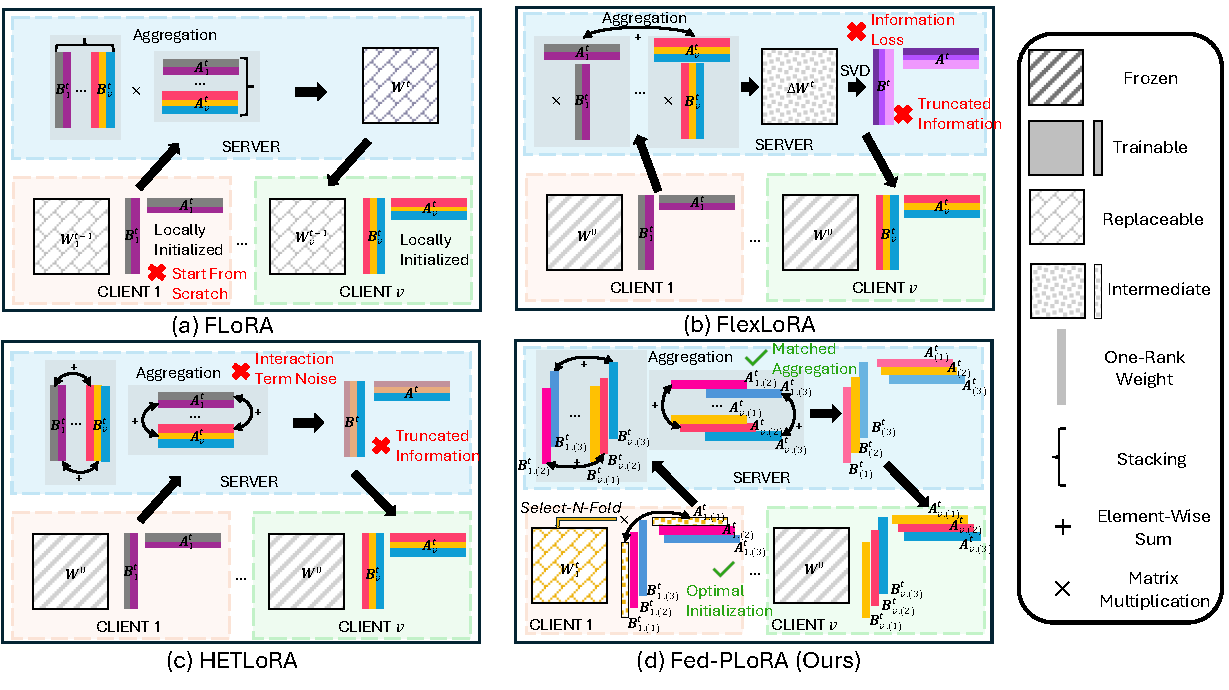
\includegraphics[width=0.92\linewidth]{fig/framework.pdf}
    \vspace{-8pt}
    \caption{Framework of FLoRA, FlexLoRA, HETLoRA, and our method Fed-PLoRA.}
    \label{fig:framework}
    \vspace{-15pt}
\end{figure*}

\subsection{Motivation}
Existing LoRA-based heterogeneous FFT methods~\cite{cho2024heterogeneous,bai2024federated,wangflora} that follow the above training framework differ primarily in their initialization and aggregation strategies.
% Many federated fine-tuning frameworks~\cite{cho2024heterogeneous,bai2024federated,wangflora} are designed for heterogeneous environments, each with different specific implementations of the $\Init$ and $\Agg$ strategies to handle heterogeneity. 
To analyze their effects, we formally define the notions of initialization noise and aggregation noise as follows: 

\textit{Initialization Noise:} During the initialization step of round $t$, clients with limited local rank $r_i$ may be unable to fully accommodate the information contained in the global LoRA modules as $r_i\leq R$. This mismatch introduces initialization noise, defined as the total initialization gap across all clients:
% 
% During the initialization step at round $t$, initialization noise can occur if clients are unable to fully utilize the information contained in the global LoRA modules due to their limited local ranks $r_i$. 
% \hl{ Question Mark: In the perspective of the optimal global LoRA modules, this is correct, right? Question Mark: Is there any Mismatch with} Eq~\ref{eq:fl_step1_init} and Eq~\ref{eq:fl_step3_agg}\hl{!?)} Let $\mathcal{K}_i^t=\{j|j=1\dots R,\mathbf{A}_{i,(j)}^t\neq\mathbf{A}_{(j)}^t \text{ or } \mathbf{B}_{i,(j)}^t\neq\mathbf{B}_{(j)}^t \}$ denote the set of indices where the initialized local LoRA module does not match the weights in the global model or not exist, where $j$ is the rank index. 
% Specifically, the initialization noise at round $t$ is defined as the sum of the initialization gap of all clients:
\begin{align}
    \mathcal{N}_{\Init}^{t} 
    % &= \sum_{i\in[v]}\left\| \left( \mathbf{B}^t\ominus \mathbf{B}_i^t\right) \left( \mathbf{A}^t\ominus \mathbf{A}_i^t\right)  \right\| \notag \\
    % & = \sum_{i\in[v]} \left\| \mathbf{B}^t_{[:,\mathcal{K}_i^t]} \mathbf{A}^t_{[\mathcal{K}_i^t,:]}  \right\|
    := 
    % \sum_{i\in[v]} \left\| \mathbf{B}^t_{(\{j|j\in\mathcal{K}_i^t\})} \mathbf{A}^t_{(\{j|j\in\mathcal{K}_i^t\})}  \right\|_F,
    \sum_{i\in[v]} \left(\left\|{\mathbf{A}}^{t-1}\ominus {\mathbf{A}}_i^{t-1}\right\|_F + \left\|{\mathbf{B}^{t-1}}\ominus {\mathbf{B}}_i^{t-1}\right\|_F\right), \label{eq:initialization_noise_truncation_sum_direct}
\end{align}
where $\| \cdot \|_F$ denotes the Frobenius norm, and the operator $\ominus$ represents a rank-wise subtraction. This metric quantifies the information that resource-constrained clients fail to retain when initializing from the global model. In homogeneous rank settings (i.e., $r_i=R$ for all $i\in[v]$), the initialization noise vanishes since all clients can directly adopt the global LoRA modules. %, indicating the challenges of preserving the quality of local training in heterogeneous settings. 
% If all clients $i \in [v]$ have $r_i=R$, then $\mathcal{N}_{\text{Init}}^{t} = 0$. 



\textit{Aggregation noise:} After local training, the server receives updated parameters $\boldsymbol{\theta}^{t}_i$ from each client $i$. Following prior works~\cite{wangflora,sun2024improving}, we define an \textit{ideal} model update $ \Delta \boldsymbol{\mathcal{W}}_*^t$ as the average of the local model updates, and the deviation from this ideal model update defines the aggregation noise, i.e., 
\begin{equation}
  \mathcal{N}_{\Agg}^{t} := \left\| \Delta {\boldsymbol{\mathcal{W}}}_{*}^{t} - \Delta {\boldsymbol{\mathcal{W}}}^{t} \right\|_F, \text{ with } \Delta {\boldsymbol{\mathcal{W}}}_*^{t } =  \frac{1}{v}\sum_{i\in [v]} \Delta {\boldsymbol{\mathcal{W}}_i^t} =  \frac{1}{v}\sum_{i\in [v]} \mathbf{B}_i^{t} \mathbf{A}_i^{t},
\end{equation}
% evaluate the aggregated LoRA product, denoted as the update to the pre-trained target module ${\boldsymbol{\mathcal{W}}^0}$,
% \begin{align}
%  {\boldsymbol{\mathcal{W}}^0}+ \Delta {\boldsymbol{\mathcal{W}}}^t &=  {\boldsymbol{\mathcal{W}}^0} + \frac{1}{v}\sum_{i\in [v]} \Delta {\boldsymbol{\mathcal{W}}_i^t} \notag\\
%  &=  {\boldsymbol{\mathcal{W}}^0} + \frac{1}{v}\sum_{i\in [v]} \mathbf{B}_i^{t} \mathbf{A}_i^{t}.
% \end{align}
% The deviation from this ideal model update defines the aggregation noise:
% \begin{align}
% \mathcal{N}_{\Agg}^{t} &:= \left\| \Delta {\boldsymbol{\mathcal{W}}}_{*}^{t} - \Delta {\boldsymbol{\mathcal{W}}}^{t} \right\|_F, \label{eq:aggregation_noise_definition}
% % &= \| \mathbf{A}^{t} \mathbf{B}^{t} - \frac{1}{|S^t|}\sum_{i\in S^t} \mathbf{B}^{t}_i \mathbf{A}_i^{t} \| 
% \end{align} 
where $\Delta\boldsymbol{\mathcal{W}}^{t}=\mathbf{B}^{t}\mathbf{A}^{t}$ represents the actual model update obtained by a specific aggregation method. Ideally, a perfect aggregation method yields $\mathcal{N}_{\Agg}^{t} = 0$. 
% Following server-side aggregation, we assume an optimal initialization method that can perfectly derive LoRA module parameters ${\mathbf{A}^*}^t$ and ${\mathbf{B}^*}^t$ from $\Delta {\boldsymbol{\mathcal{W}}^*}^t$, which then distributed to the clients according to client's rank $r_i$. As indicated in Equation~\eqref{eq:optimal_grad_A_intro}, an optimal gradient of client $i$ accounts for the optimal LoRA module weights and optimal loss. Let ${\mathcal{L}^*}_i^{t+1}$ denotes the local loss for client $i$ in round $t+1$. The optimal target gradient with respect to ${\mathbf{A}^*}_i^{t+1}$, computed using the optimal parameters $ {\mathbf{B}^*}_i^{t+1}$, would be $\nabla_{{\mathbf{A}^*}_i^{t+1}} {\mathcal{L}^*}_i^{t+1}$.
% \hl{In practice, a specific $\Agg$ method employed by the server produces an actual aggregated LoRA update product, $\Delta \boldsymbol{\mathcal{W}}^{\prime t}$, which may not result in an optimal aggregation.}
% However, a actual initialization method might provide client $i$ with actual parameters $(\mathbf{A}_i^{t+1}, \mathbf{B}_i^{t+1})$ for round $t+1$. 

% The initialization noise for client $i$ is defined as the deviation of the gradient computed with the actual parameters from the gradient computed with the optimal target parameters for that round:

% \begin{align}
% \mathcal{N}_{\mathrm{Init},i}^{t+1}
% = &\Bigl\lVert
%      \nabla_{\mathbf{A}_i^{*\,t+1}}{\mathcal{L}^*}_i^{t+1}
%      - \nabla_{\mathbf{A}_i^{t+1}}\mathcal{L}_i^{t+1}
%    \Bigr\rVert_{F} \\
% \quad + &\Bigl\lVert
%      \nabla_{\mathbf{B}_i^{*\,t+1}}{\mathcal{L}^*}_i^{t+1}
%      - \nabla_{\mathbf{B}_i^{t+1}}\mathcal{L}_i^{t+1}
%    \Bigr\rVert_{F}.\notag
% \end{align}
% This definition quantifies how far the client's starting optimization in round $t+1$ (using actual parameters $(\mathbf{A}_i^{t+1}, \mathbf{B}_i^{t+1})$) is from an ideal optimization trajectory
% An ideal initialization method yield $\mathcal{N}_{\text{Init},i}^{t+1} = 0$.

% It is important to note that the overall impact on clients' training can propagate from either aggregation noise (if $\Delta\mathbf{W}_{}^{t} \neq \Delta{\mathbf{W}^*}^{t}$, meaning the basis for deriving $({\mathbf{A}^*}_i^{t+1}, {\mathbf{B}^*}_i^{t+1})$ is already sub-optimal) or initialization noise (if the distributed modules $(\mathbf{A}_i^{t+1}, \mathbf{B}_i^{t+1})$ do not lead to gradients matching those from perfectly derived $({\mathbf{A}^*}_i^{t+1}, {\mathbf{B}^*}_i^{t+1})$), or both. 

% Overall, this analysis allows us to systematically evaluate how existing methods lead to these noise components. In the next section, xxx


% We aim to design a new FFT method that achieves minimal xxx noises. 
% Therefore, to improve FFT performance, it is essential to reduce the xxx noise. 
% To reveal the causes of performance degradation in heterogeneous FFT, we introduce formal definitions of initialization and aggregation noise. These formulations motivate the design of Fed-PLoRA by emphasizing the need to reduce both initialization mismatch and aggregation deviation caused by rank heterogeneity.

\subsection{Parallel One-Rank Adaptation}\label{plora}


Before presenting the Fed-PLoRA framework, we first introduce its fundamental building block, PLoRA. The key idea is to replace a single multi-rank LoRA module with multiple parallel one-rank modules. 
% 
Concretely, consider applying a LoRA module with rank $R$ to a target weight matrix $\boldsymbol{\mathcal{W}}^0 \in \mathbb{R}^{d \times k}$. In classical LoRA, this is parameterized by matrices $\mathbf{A} \in \mathbb{R}^{R \times k}$ and $\mathbf{B} \in \mathbb{R}^{d \times R}$, yielding the update $\Delta\boldsymbol{\mathcal{W}}_{\text{LoRA}} := \mathbf{B}\mathbf{A}$. In contrast, PLoRA decomposes this rank-$R$ module into $R$ parallel one-rank components. For each $j \in [R]$, a PLoRA component consists of a pair of one-rank matrices $\mathbf{A}_{(j)} \in \mathbb{R}^{1 \times k}$ and $\mathbf{B}_{(j)} \in \mathbb{R}^{d \times 1}$ (see Figure~\ref{fig:framework}(d)), producing an individual update $\Delta\boldsymbol{\mathcal{W}}_{(j)} =  \mathbf{B}_{(j)}\mathbf{A}_{(j)}$. The overall update is simply the sum of these contributions: 
\[
\Delta\boldsymbol{\mathcal{W}}_{\text{PLoRA}} := \sum_{j=1}^R\Delta\boldsymbol{\mathcal{W}}_{(j)} = \sum_{j=1}^R \mathbf{B}_{(j)}\mathbf{A}_{(j)} =   \sum_{j=1}^R \mathbf{B}_{[:,j]} \mathbf{A}_{[j,:]} =\Delta\boldsymbol{\mathcal{W}}_{\text{LoRA}}
\] 
which is mathematically equivalent to the classic multi-rank LoRA formulation, since $\mathbf{B}{(j)} = \mathbf{B}{[:,j]}$ and $\mathbf{A}{(j)} = \mathbf{A}{[j,:]}$. 
% \[
% \Delta\boldsymbol{\mathcal{W}} = \mathbf{B} \mathbf{A} = \sum_{j=1}^R \mathbf{B}_{[:,j]} \mathbf{A}_{[j,:]},
% \]
% where $\mathbf{B}_{[:,j]}$ is the $j$-th rank of $\mathbf{B}$ and where $\mathbf{A}_{[j,:]}$ is the $j$-th rank of $\mathbf{A}$. 
Thus, PLoRA achieves the same adaptation effect and parameter efficiency as standard multi-rank LoRA, while enabling a modular decomposition that is naturally suited to heterogeneous FTT.

% to apply a LoRA module with rank $R$ for the target module $\boldsymbol{\mathcal{W}}^0\in\mathbb{R}^{d\times k}$, classic LoRA configures matrices ${\mathbf{A}}\in\mathbb{R}^{R \times k}$ and ${\mathbf{B}}\in\mathbb{R}^{d \times R}$. In contrast, Fed-PLoRA utilizes $R$ parallel, one-rank modules. For $j\in[R]$, each module consists of a pair of one-rank matrices  $\mathbf{A}_{(j)}\in\mathbb{R}^{1 \times k} $ and $\mathbf{B}_{(j)}\in\mathbb{R}^{d \times 1}$ (as illustrated in Figure~\ref{fig:framework} (d)). Each pair $\{\mathbf{A}_{(j)}, \mathbf{B}_{(j)}\}$ results in an individual update $\Delta\boldsymbol{\mathcal{W}}_{(j)} =  \mathbf{B}_{(j)}\mathbf{A}_{(j)}$ to the target module. With $R$ such PLoRA module pairs, the total update $\Delta\boldsymbol{\mathcal{W}}$ to the target module is the sum of these individual updates: $\Delta\boldsymbol{\mathcal{W}} = \sum_{j=1}^R\Delta\boldsymbol{\mathcal{W}}_{(j)} = \sum_{j=1}^R \mathbf{B}_{(j)}\mathbf{A}_{(j)}$. 

% Compared to the conventional multi-rank adaptation  $\boldsymbol{\mathcal{W}}^0 + \Delta\boldsymbol{\mathcal{W}} = \boldsymbol{\mathcal{W}}^0 + \mathbf{B} \mathbf{A}$, which can be expressed as $ \boldsymbol{\mathcal{W}}^0 + 
%  \sum_{j=1}^R \mathbf{B}_{[:,j]} \mathbf{A}_{[j,:]}$ where $\mathbf{B}_{[:,j]}$ is the $j$-th rank of $\mathbf{B}$ and where $\mathbf{A}_{[j,:]}$ is the $j$-th rank of $\mathbf{A}$, this parallel one-rank adaptation achieves an identical adaptation effect as the multi-rank adaptation with the same parameter efficiency. 

% Let ${\mathbf{A}}:= \{ \mathbf{A}_{(j)}\in\mathbb{R}^{1 \times k}\}_{j=1}^R$ and ${\mathbf{B}}:= \{ \mathbf{B}_{(j)}\in\mathbb{R}^{1 \times k}\}_{j=1}^R$ 



\subsection{Fed-PLoRA: Heterogeneous FFT with PLoRA}

As in existing approaches, resource-constrained clients can reduce their LoRA ranks to fit limited computational budgets, which naturally results in heterogeneous ranks across clients. Within our framework, this corresponds to adjusting the number of parallel one-rank matrix pairs in the PLoRA modules. However, this adjustment alone does not eliminate initialization and aggregation noise.

%In the context of our method, it can be achieved by adjusting the number of parallel one-rank matrix pairs within the PLoRA modules. However, it does not inherently mitigate initialization and aggregation noise.
To overcome these issues in heterogeneous settings, we propose a novel \textit{Select-N-Fold} strategy within the Fed-PLoRA framework. This strategy is specifically designed to handle rank heterogeneity, ensuring zero initialization noise and minimizing aggregation noise. 
% To address these persistent issues in heterogeneous environments, we introduce a novel \textit{Select-N-Fold} strategy in our Fed-PLoRA framework. This strategy is specifically designed to effectively manage rank heterogeneity, aiming for zero initialization noise and minimal aggregation noise. 
% 
Assume the server maintains global PLoRA parameters $\boldsymbol{\theta} = \{\{\mathbf{A}^l\}_{l\in[L]}, \{\mathbf{B}^l\}_{l\in[L]} \}$, where for each target module $l\in [L]$, ${\mathbf{A}^l} := \{ \mathbf{A}_{(j)}^l\}_{j\in[R]}$ and ${\mathbf{B}^l} := \{ \mathbf{B}_{(j)}^l\}_{j\in[R]}$ represent the $R$ parallel one-rank PLoRA components. For client $i$, the local PLoRA parameters are $\boldsymbol{\theta}_i = \{\{\mathbf{A}_i^l\}_{l\in[L]}, \{\mathbf{B}_i^l\}_{l\in[L]}\}$, where ${\mathbf{A}_{i}^l} := \{ \mathbf{A}_{i,(j)}^l\}_{j\in[r_i]}$ and ${\mathbf{B}_{i}^l} := \{ \mathbf{B}_{i,(j)}^l\}_{j\in[r_i]}$ with local rank $r_i$. The global rank is chosen such that $R \geq \max_{i \in [v]} r_i$. 
% 
Fed-PLoRA follows the three-step training framework described in Section~\ref{sec:system_formula}, and the pseudo-code is shown in Algorithm~\ref{algorithm-ours}. In each training round $t$:

% Assume the server maintains the global PLoRA parameters $\boldsymbol{\theta} = \{\mathbf{A}, \mathbf{B}\}$, where ${\mathbf{A}} := \{ \mathbf{A}_{(j)}\}_{j=1}^R$ and ${\mathbf{B}}:= \{ \mathbf{B}_{(j)}\}_{j=1}^R$ represent the $R$ parallel one-rank matrix pairs. 
% For each client $i$, it maintains the local PLoRA parameters $\boldsymbol{\theta}_i = \{\mathbf{A}_i, \mathbf{B}_i\}$, where ${\mathbf{A}_{i}} := \{ \mathbf{A}_{i,(j)}\}_{j=1}^{r_{i}}$ and ${\mathbf{B}_{i}} := \{ \mathbf{B}_{i,(j)}\}_{j=1}^{r_{i}}$ with their specific rank $r_i$.
% Here, the global rank $R$ should satisfy $R\geq \max\{r_i, i\in[v]\}$. Fed-PLoRA follows the three-step training framework in the last section. In each training round:



\textbf{Broadcast and Initialization:} The server broadcasts the global PLoRA parameters $\boldsymbol{\theta}^{t-1}$ to clients. 
Each client $i$ then randomly selects a subset $\mathcal{K}_i^{t}$ of $r_i$ parallel one-rank PloRA modules for local training. For clarity, we omit the index $l$ in the notation, but note that this selection and the subsequence operations are performed independently for each target module $l \in [L]$. The local PLoRA parameters of client $i$ are initialized as $\boldsymbol{\theta}_i^{t-1} = \{\mathbf{A}_{(j)}^{t-1}, \mathbf{B}_{(j)}^{t-1} \}_{j\in \mathcal{K}_i^{t}}$. 
The remaining $(R-r_i)$ parallel one-rank PLoRA modules are temporarily \textbf{folded} into the corresponding pre-trained target module $\boldsymbol{\mathcal{W}}^0$, {yielding the local target module }
\[
\boldsymbol{\mathcal{W}}_i^{t} := \boldsymbol{\mathcal{W}}^0 + \Delta\boldsymbol{\mathcal{W}}_{\text{fold},i}^{t-1} = \boldsymbol{\mathcal{W}}^0 + \sum_{j\notin \mathcal{K}_i^{t}} \mathbf{B}_{(j)}^{t-1}\mathbf{A}_{(j)}^{t-1},
\]
which then remains frozen during local training. 
% 
% Specifically, the collective update derived from these unselected modules is $\Delta\boldsymbol{\mathcal{W}}_{\text{fold},i}^{t-1} := \sum_{j\notin \mathcal{K}_i^{t}} \mathbf{B}_{(j)}^{t-1}\mathbf{A}_{(j)}^{t-1}$. The client then adds this update to the target module such that $\boldsymbol{\mathcal{W}}_i^t = \boldsymbol{\mathcal{W}}^0 + \Delta\boldsymbol{\mathcal{W}}_{\text{fold},i}^{t-1}$. 
% Note that the folding process is always applied to the pre-trained target module $\boldsymbol{\mathcal{W}}^0$, and the resulting $\boldsymbol{\mathcal{W}}_i^t$ remains frozen during local training.
% 
This procedure allows the client to preserve information from the full set of global PloRA modules while training only a subset. Consequently, client $i$ operates with an effective rank of $r_i$, matching the parameter count of a standard rank-$r_i$ LoRA configuration, but without incurring initialization noise. 
% It ensures that the number of trainable parameters for client $i$ corresponds to an effective LoRA rank of $r_i$, matching that of a standard LoRA configuration of rank $r_i$, while avoiding any initialization noise.


\textit{Randomness in Select-N-Fold:} Our objective is to obtain a well-trained global PLoRA that can be applied to the pretrained backbone for downstream tasks. When local resource is sufficient (i.e., $r_i = R$), all local PLoRA modules can be trained, ensuring that every global PLoRA module is updated. When $r_i < R$, trainable modules are selected independently across clients and target modules; hence, in expectation, each global module is updated by some subset of clients in every round. This randomness mitigates the risk of long-term staleness in global PLoRA modules under the Select-N-Fold strategy. %Empirical results further demonstrate the effectiveness of random selection compared to adaptive selection strategies (see \supplement{Appendix Section~\ref{appendixsubsection:selection}}). 


% \textit{Justification for Random Selection:} To ensure that all global one-rank matrix pairs receive sufficient training over time, random selection is performed independently for each client in every round. This mechanism increases the likelihood that all one-rank matrix pairs on the server are eventually updated by a subset or all of the participating clients, thereby avoiding long-term staleness in folded modules. We empirically validate this in \supplement{Appendix Figure~\ref{fig:vis_selection}} by reporting per-rank update frequencies across training rounds. Discussions on other selection adaptive strategies are provided in \supplement{Appendix Section~\ref{appendixsubsection:selection}}. 
 
% In this case, the number of local PLoRA parameters with rank $r_i$ is equivalent to that of classic LoRA parameters with the same rank.  % in the existing methods such as FLoRA, FlexLoRA and HETLoRA. 
% The core idea of Fed-PLoRA is the utilization of multiple parallel, one-rank LoRA modules instead of a single, multi-rank module for each target module.  %
% As illustrated in Figure~\ref{fig:framework} (d), for each target module $\boldsymbol{\mathcal{W}}^0 \in \mathbb{R}^{d \times k}$, Fed-PLoRA introduces $R$ parallel one-rank LoRA modules on client $i$. Each pair of parallel module $\mathbf{A}_{i,(j)}^t\in\mathbb{R}^{1\times k},\mathbf{B}_{i,(j)}^t\in\mathbb{R}^{d\times 1},j \in [r_i]$ is defined by a pair of one-rank matrices $(\mathbf{B}_{i,(j)} \in \mathbb{R}^{d \times 1}, \mathbf{A}_{i,(j)} \in \mathbb{R}^{1 \times k})$. 
% The output on client $i$ is formulated as $\hat{y}_i = \boldsymbol{\mathcal{W}}^{0} x +\sum_{j=0}^{R-1} \mathbf{B}_{i,(j)} \mathbf{A}_{i,(j)} x$ with an input $x$.

% This architecture provides a flexible way for clients to adapt their trainable parameters to the specific resource constraints, while also creating a way to reduce initialization and aggregation noise. 
% The total LoRA update for $\boldsymbol{\mathcal{W}}^0$ is then the sum of the products of these parallel modules: $\Delta\boldsymbol{\mathcal{W}} = \sum_{j=0}^{R-1} \mathbf{B}_{(j)}\mathbf{A}_{(j)}$.

% \textbf{Initialization:} As shown in Figure~\ref{fig:framework} (d), we initialize the local models by introducing a \textit{Select-N-Fold} strategy. Specifically, after receiving LoRA modules from the server, each client $i$ randomly chooses $r_i$ parallel LoRA modules to be trainable at the beginning of each round. 

% This provides fine-grained control over the number of trainable parameters per client. 

% To further reduce the extra forward computational costs (from frozen LoRA modules) during fine-tuning, clients merge their frozen parallel LoRA module weights into the target module. In detail, let the trainable subset of parallel modules be denoted as $C_{i,T}^t$, and the frozen subset as $C_{i,F}^t$. The target module is then formulated as $\boldsymbol{\mathcal{W}}_i^t=\boldsymbol{\mathcal{W}}^{0}+\sum_{i\in C_{i,F}^t}\mathbf{B}_{i,(j)}^t\mathbf{A}_{i,(j)}^t$, such that the output on client $i$ is formulated as $\hat{y}_i = \boldsymbol{\mathcal{W}}^{t}_i x +\sum_{j\in C_{i,T}^t} \mathbf{B}_{i,(j)} \mathbf{A}_{i,(j)} x$ with an input $x$. In this way, the additional computational cost is avoided.



\textbf{Local Client Update:} During local training, each client $i$ updates only the selected PLoRA modules in $\mathcal{K}_i^{t}$. After optimization, the updated local PLoRA parameters are $\boldsymbol{\theta}_i^t=\{{\mathbf{A}_{i,(j)}^{t},\mathbf{B}_{i,(j)}^{t}}\}_{j\in\mathcal{K}_i^{t}}$, which are then transmitted to the server.


\textbf{Server-Side Aggregation:} The server aggregates these local PLoRA modules in a rank-wise manner. For each $j\in[R]$, the global PLoRA modules are computed as ${\mathbf{A}}^t_{(j)}=\frac{1}{|\mathcal{Q}^t_{(j)}|}\sum_{i\in{\mathcal{Q}^t_{(j)}}}\mathbf{A}_{i,(j)}^{t}$, ${\mathbf{B}}^t_{(j)}=\frac{1}{|\mathcal{Q}^t_{(j)}|}\sum_{i\in{\mathcal{Q}^t_{(j)}}}\mathbf{B}_{i,(j)}^{t}$, where $\mathcal{Q}^t_{(j)}=\{i|i\in[v],j\in\mathcal{K}_i^{t} \}$ denotes the set of clients that updated module $j$ in round $t$. The aggregated global PLoRA parameters $\boldsymbol{\theta}^{t} = \{\mathbf{A}^t, \mathbf{B}^t\}$ are then used for the next round of training. The process iterates until the global model converges. 


% \textit{Computational and communication costs of clients.}
% In Fed-PLoRA, the computational and uplink communication cost (in terms of the number of trainable parameters) for each client scales linearly with its selected rank $r_i$, since only $r_i$ one-rank modules are updated per round. This is comparable to existing methods like FedIT. 

% Note that the additional folding step incurs negligible overhead relative to local training. 

% In Fed-PLoRA, each one-rank PLoRA module is highly lightweight (two vectors of dimensions $d$ and $k$), and the total downlink payload scales as ${O}((d+k)R)$. Since all our method is built on parameter-efficient fine-tuning, the global rank $R$ remains small in practice. 

% This is slightly higher than methods such as HETLoRA and FlexLoRA, which only send rank-$r_i$ modules to each client. However, since downlink communication is typically far cheaper than uplink in federated settings~\cite{mhanna2024countering}, and low-rank adaptation is inherently parameter-efficient, the additional downlink cost that scales linearly with $(R-r_i)$ remains modest. 

% We provide xxx in Section~\ref{} with several real-world examples. 



% \textbf{Intuition for Stable Aggregation.} 

% The design of Fed-PLoRA is motivated by sparse training~\cite{ardakani2024slimfit}, which keep the same model structure but tra. This is unlike methods that might force heterogeneous updates into a single, monolithic LoRA structure, potentially losing nuanced information or causing interference between disparate update components.

% \begin{tcolorbox}[colback=white, colframe=red!70!black, boxrule=0.8pt, arc=2mm, title={\textbf{Insight}}] % Added 
% % \includegraphics[height=1.5em]{fig/insight.png} 
% In a running relay, different runners have their own strengths (e.g., straight speeding, bend running, or reliable receiving). If any runner is missing, and one has to run two legs, the team would likely lose the race. Similarly, each parallel LoRA module in Fed-PLoRA can be conceptualized as a specialized ``runner'' contributing a unique aspect to the overall model feature. Instead of totally missing during race, couple of missing during practice is not too harmful.
% \end{tcolorbox}

% \begin{tcolorbox}[colback=white, colframe=red!70!black, boxrule=0.8pt, arc=2mm]
% \includegraphics[height=1.5em]{fig/insight.png} \textbf{Insight:} In a running relay, different runners have their own strengths (e.g., straight speeding, bend running, or reliable receiving). If any runner is missing, and one has to run two legs, the team would lose the race.
% \end{tcolorbox}


\subsection{Analysis of Initialization and Aggregation Noise}\label{subsec:baselines}
\begin{wrapfigure}{r}{0.60\textwidth} 
\vspace{-20pt}
    \centering
    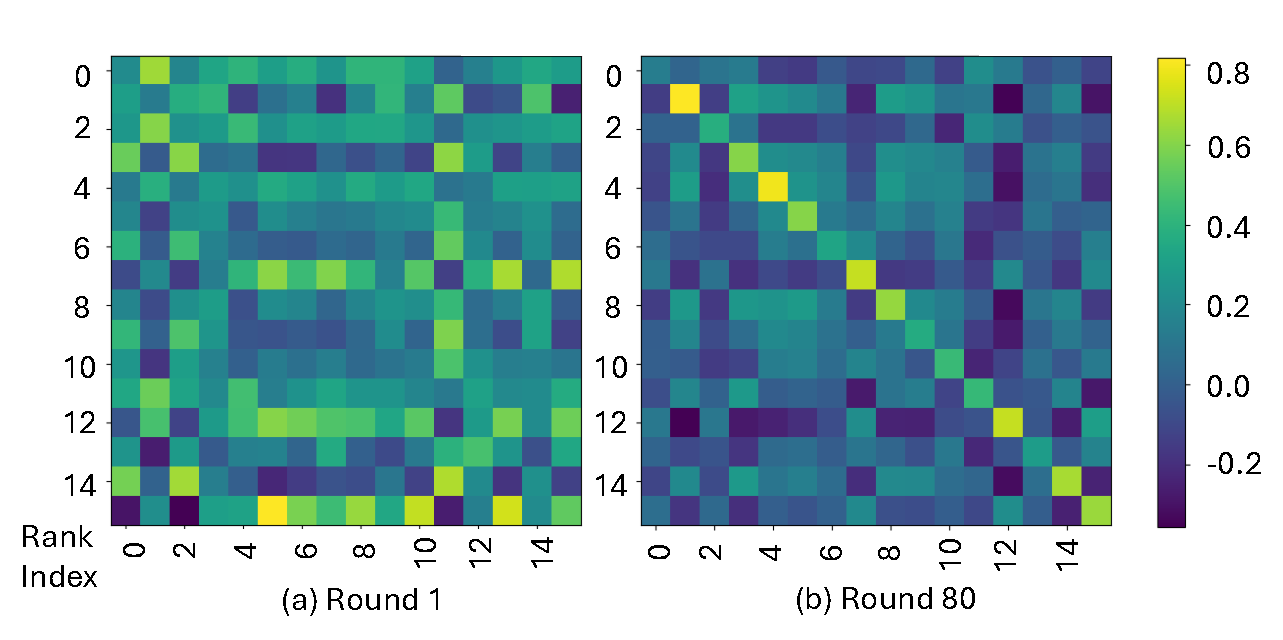
\includegraphics[width=\linewidth]{fig/emprical.pdf}
    \vspace{-10pt}
    \caption{Cosine similarities between parallel one-rank modules of PLoRA. 
    (a) Low, random similarities at initialization; (b) Increasing within-rank similarity across clients, while cross-rank similarity remains low, indicating that modules capture distinct knowledge at different ranks but converge on similar knowledge across clients, despite differences in resource limitations and data distributions (see \supplement{Appendix Section~\ref{appendixsubsection:other_settings}}).}
    \label{fig:aggregation_noise}
  \vspace{-20pt}
\end{wrapfigure}
Here, we analyze the initialization and aggregation noise of Fed-PLoRA, comparing it with three SOTA methods, FLoRA~\cite{wangflora}, FlexLoRA~\cite{bai2024federated}, and HETLoRA~\cite{cho2024heterogeneous}. Due to page limitations, we provide the detailed derivation in Appendix~\ref{appendixsec:analysis}. 

\textbf{Fed-PLoRA.} Because each client either trains or folds the globally initialized one-rank modules into its frozen target weights, there is no discrepancy between local and global modules. Hence, $\mathcal{N}_{\text{Ours\_}\Init}^{t} = 0$. 
%In our method, all $R$ global PLoRA modules \hu{how does Fed-PLoRA behave when the global rank is very large—does communication overhead become prohibitive?} are either selected for local training or folded into the frozen target module $\boldsymbol{\mathcal{W}}_i^t$, both initialized from the global state. Since no discrepancy between global and local modules, the initialization noise $\mathcal{N}_{\text{Ours\_}\Init}^{t} = 0$.
% 
Under our aggregation rule, the aggregation noise is 
$
   \mathcal{N}_{\text{Ours\_Agg}}^{t}   =  \| \sum_{j=1}^{R}(({1}/{|\mathcal{Q}_{(j)}^t|}) \sum_{i \in \mathcal{Q}_{(j)}^t} (\mathbf{B}_{i,(j)}^{t} - \overline{\mathbf{B}}_{(j)}^t)(\mathbf{A}_{i,(j)}^{t} - \overline{\mathbf{A}}_{(j)}^t) )\|_F,
   \label{eq:agg_noise_plora}
$
where $\overline{\mathbf{A}}_{(j)}^t := ({1}/{|\mathcal{Q}_{(j)}^t|})\sum_{i \in \mathcal{Q}_{(j)}^t} \mathbf{A}_{i,(j)}^t$ 
and $\overline{\mathbf{B}}_{(j)}^t := ({1}/{|\mathcal{Q}_{(j)}^t|}) \sum_{i \in \mathcal{Q}_{(j)}^t} \mathbf{B}_{i,(j)}^t$. This noise vanishes when the cross-client covariance between $\mathbf{A}_{i,(j)}^t$ and $\mathbf{B}_{i,(j)}^t$ is zero for every rank. More generally, by the Cauchy–Schwarz inequality, it can be bounded as 
$
\mathcal{N}_{\text{Ours\_Agg}}^{t}  \leq \sum_{j=1}^{R}\frac{1}{|\mathcal{Q}_{(j)}^t|} \sum_{i \in \mathcal{Q}_{(j)}^t} \|  \mathbf{B}_{i,(j)}^{t} - \overline{\mathbf{B}}_{(j)}^t \|_2 + \| \mathbf{A}_{i,(j)}^{t} - \overline{\mathbf{A}}_{(j)}^t\|_2.
$
As shown in the heatmap in Figure~\ref{fig:aggregation_noise}, the diagonal entries represent the similarity of the $j$-th PLoRA module ($j \in [R]$) across clients, averaged over all client pairs. 
We observe that these similarities increase significantly as training progresses, indicating that local PLoRA modules become more aligned across clients. This alignment reduces deviations from the mean, thereby tightening the upper bound of the aggregation noise. 
% \begin{align}\label{eq:agg_noise_plora}
% \mathcal{N}_{\text{Ours\_Agg}}^{t}  
% =&\left\| \sum_{j=1}^{R} \frac{1}{|\mathcal{Q}_{(j)}^t|^2} \left( 
% \sum_{i_1 \in \mathcal{Q}_{(j)}^t} \sum_{i_2 \in \mathcal{Q}_{(j)}^t} 
% \mathbf{B}_{i_1,(j)}^{t} \mathbf{A}_{i_2,(j)}^{t} \right. \right. 
% % \notag \\
% % &\quad \left. \left. 
% \left. \left.
% - |\mathcal{Q}_{(j)}^t| \sum_{i \in \mathcal{Q}_{(j)}^t} 
% \mathbf{B}_{i,(j)}^{t} \mathbf{A}_{i,(j)}^{t} 
% \right) \right\|_F
% \end{align}
% The detailed derivations is provided in \supplement{Appendix Section~\ref{appendixsubsection:fedplora}}. 

% $\frac{1}{|\mathcal{Q}_{(j)}^t|} \sum_{i \in \mathcal{Q}_{(j)}^t} \left(\mathbf{B}_{i,(j)}^{t} - \overline{\mathbf{B}}_{(j)}^t\right)\left(\mathbf{A}_{i,(j)}^{t} - \overline{\mathbf{A}}_{(j)}^t\right) = \mathbf{0}$. 

% , where 

% $\overline{\mathbf{A}}_{(j)}^t := \frac{1}{|\mathcal{Q}_{(j)}^t|} \sum_{i \in \mathcal{Q}_{(j)}^t} \mathbf{A}_{i,(j)}^t$ 
% and $\overline{\mathbf{B}}_{(j)}^t := \frac{1}{|\mathcal{Q}_{(j)}^t|} \sum_{i \in \mathcal{Q}_{(j)}^t} \mathbf{B}_{i,(j)}^t$ are the average of $\mathbf{A}_{i,(j)}^t$ and  $\mathbf{B}_{i,(j)}^t$ across clients for module $j$ at round $t$, respectively. 


% We conduct a qualitative study on LoRA module weights during training under a non-IID setting (check \supplement{Appendix Section~\ref{appendixsubsection:other_settings}} for experimental setup). As shown in Figure~\ref{fig:aggregation_noise}, we visualize the pairwise cosine similarities between PLoRA $\mathbf{A}_{i,(j)}^t$ module weights. In the heatmap, both rows and columns correspond to clients' LoRA modules at index $j$. Each cell shows the average cosine similarity between $j$-th LoRA module weights from client $i_1$ and client $i_2$, where $ i_1, i_2 \in [v] $ and $ i_1 \ne i_2 $. This captures how consistently different clients update the same-index LoRA module. In Figure~\ref{fig:aggregation_noise} (a), in the early training stage, each parallel LoRA module from clients barely shows any similarities. However, as illustrated in Figure~\ref{fig:aggregation_noise} (b), in the late training round, each client focuses on capturing similar features in the parallel modules at the same index $j$. When the cosine similarity among all local LoRA matrices $\mathbf{A}_{i,(j)}^t$ within group $j$ is high, it implies that these matrices are nearly aligned in direction. In such a case, we can approximate:
% \begin{align}\label{eq:plora_noise_0_a}
% \mathbf{A}_{i,(j)}^t \approx \overline{\mathbf{A}}_{(j)}^t \quad \forall i \in \mathcal{Q}_{(j)}^t,
% \end{align}
% results in a small aggregation noise. For more visualizations and discussions, please refer to \supplement{Appendix Section~\ref{appendixsubsection:vis_cos_sim}}.
% \hl{Need to explain why this happens? How?}

% Overall, our method achieves optimal initialization and significantly reduces aggregation noise.

% \subsection{Limitation of Existing Methods}\label{subsec:baselines}
% While the optimal scenario outlined in Section~\ref{subsec:optimal_benchmark} provides a useful mathematical reference, practical heterogeneous federated fine-tuning methods often introduce noise due to their specific initialization and aggregation mechanisms. 
% In this section, we examine the sources of initialization and aggregation noise in three representative frameworks, FLoRA~\cite{wangflora}, FlexLoRA~\cite{bai2024federated}, and HETLoRA~\cite{cho2024heterogeneous} in the literature, as illustrated in Figure~\ref{fig:framework}. 


% Overall, our method achieves zero initialization noise and exhibits minimal aggregation noise.  
% In the following paragraphs, we analyze both types of noise in SOTA methods for comparison.  
% Detailed mathematical derivations for these methods are provided in \supplement{Appendix Sections~\ref{appendixsec:analysis}}.

% The detailed mathematical derivations for these methods are shown in the \supplement{Appendix Sections~\ref{appendixsec:analysis}}.

% \begin{figure}

% \end{figure}

\textbf{FLoRA.} As shown in Figure~\ref{fig:framework} (a), FLoRA employs a stacking-based aggregation method to accommodate LoRA modules from clients with heterogeneous ranks. Each client $i$ initializes its trainable LoRA modules $\{\mathbf{A}_i^{t-1}, \mathbf{B}_i^{t-1}\}$ with rank $r_i$ from scratch (e.g., $\mathbf{A}_i^{t-1}$ drawn from a normal distribution and $\mathbf{B}_i^{t-1}$ set to zeros). Before local training, the local target module is replaced with the latest global target module from the server. After local training, the updated LoRA modules $\{\mathbf{A}_i^t, \mathbf{B}_i^t\}$ are sent to the server, which concatenates all client updates along the rank dimension to form two large intermediate matrices: $\{\mathbf{A}^t\in\mathbb{R}^{(\sum_{i\in[v]}r_i)\times k},\mathbf{B}^t \in\mathbb{R}^{d\times (\sum_{i\in[v]}r_i)}\}$. The global update is then computed as $\Delta\boldsymbol{\mathcal{W}}_{\text{FLoRA}}^t = \mathbf{B}^t \mathbf{A}^t / v$. Because local LoRA modules $(\mathbf{A}_i^{t-1}, \mathbf{B}_i^{t-1})$ are freshly initialized each round, the initialization noise is $\mathcal{N}_{\text{FLoRA\_}\Init}^{t} = \sum_{i\in[v]} \left( \left\|{\mathbf{A}}^{t-1} \right\|_F+\left\|{\mathbf{B}}^{t-1} \right\|_F  \right) + \sigma^2$, where $\sigma^2$ reflects the variance of the random initialization for $\mathbf{A}$. This noise can be substantial and may degrade local training performance. On the other hand, the stacking operation in FLoRA preserves the local updates without distortion, leading to zero aggregation noise, i.e., $\mathcal{N}_{\text{FLoRA\_Agg}}^{t} = 0$. 


% The local trainable LoRA modules $\{\mathbf{A}_i^{t-1} \in\mathbb{R}^{r_i\times k}, \mathbf{B}_i^{t-1} \in \mathbb{R}^{d\times r_i}\}$ are initialized from scratch (e.g., $\mathbf{A}_i^{t-1}$ from a normal distribution, $\mathbf{B}_i^{t-1}$ as zeros). 

% Before local training, the local target module is replaced by the latest global target module downloaded from the server. After local training, the updated local LoRA modules $\{\mathbf{A}_i^{t}, \mathbf{B}_i^{t}\}$ are sent to the server. These LoRA modules from all clients are then concatenated along their rank dimension to form two large intermediate matrices $\{\mathbf{A}^t\in\mathbb{R}^{(\sum_{i\in[v]}r_i)\times k},\mathbf{B}^t \in\mathbb{R}^{d\times (\sum_{i\in[v]}r_i)}\}$. The update to the target module is obtained as $\Delta\boldsymbol{\mathcal{W}}_{\text{FLoRA}}^t = \mathbf{B}^t \mathbf{A}^t / v$.
% % , which is then used to update the global target module.

% \textit{Initialization Noise:} As the local LoRA modules $(\mathbf{A}_i^{t-1}, \mathbf{B}_i^{t-1})$ are randomly initialized, the initialization noise in expectation is
% $\mathcal{N}_{\text{FLoRA\_}\Init}^{t} = \sum_{i\in[v]} \left( \left\|{\mathbf{A}}^{t-1} \right\|_F+\left\|{\mathbf{B}}^{t-1} \right\|_F  \right) + \sigma^2$, where $\sigma^2$ denotes the magnitude of the random noise used for initializing $\mathbf{A}$ matrix. This noise can be substantial and potentially degrade local training performance.
% $\mathcal{N}_{\text{FLoRA\_}\Init}^{t} =  \sum_{i\in[v]} \left(\left\|{\mathbf{B}}^{t-1}\ominus {\mathbf{B}}_i^{t-1}\right\|_F + \left\|{\mathbf{A}^{t-1}}\ominus {\mathbf{A}}_i^{t-1}\right\|_F\right) $.
% $\mathcal{N}_{\text{FLoRA\_}\Init}^{t} = \sum_{i\in[v]} \left\| \mathbf{B}^t \mathbf{A}^t  \right\|_F$.

% In this scenario, the output $\hat{y}_i^{t+1} = \left(\boldsymbol{\mathcal{W}}^{0} +\Delta\boldsymbol{\mathcal{W}}_{\text{FLoRA}}^t \right)x + {\mathbf{B}}_i^{t+1} {\mathbf{A}}_i^{t+1} x$, equal to ${\hat{y}}_i^{*t+1}$, which results in optimal loss. However, the actual initialized parameters $(\mathbf{A}_i^{t+1}, \mathbf{B}_i^{t+1})$ are entirely independent of any optimal parameters $({\mathbf{A}_i^*}^{t+1}, {\mathbf{B}_i^*}^{t+1})$ that can be derived from $\Delta{\boldsymbol{\mathcal{W}}^*}^{t}$. Consequently, the gradients $\nabla_{\mathbf{A}_i^{t+1}}\mathcal{L}_i$ and $\nabla_{\mathbf{B}_i^{t+1}}\mathcal{L}_i$ computed at the start of round $t+1$ will be based on these random initializations and differ substantially from any optimal target gradients $\nabla_{{\mathbf{A}^*}_i^{t+1}}\mathcal{L}_i^*$ and $\nabla_{{\mathbf{B}^*}_i^{t+1}}\mathcal{L}_i^*$. 
% This results in a large $\mathcal{N}_{\text{FLoRA\_Init},i}^{t+1}$. The client's optimization trajectory is thus abruptly reset, losing any adaptation achieved by its specific LoRA modules in the previous round.

% \textit{Aggregation Noise:} The stacking operation in FLoRA allows the server to accurately average the local updates and incurs no aggregation noise such that $\mathcal{N}_{\text{FLoRA\_Agg}}^{t} = 0$.


\textbf{FlexLoRA.} 
As shown in Figure~\ref{fig:framework} (b), FlexLoRA applies singular value decomposition (SVD) to the global target module update $\Delta\boldsymbol{\mathcal{W}}^{t-1}$ to construct global LoRA modules $\{\mathbf{A}^{t-1}, \mathbf{B}^{t-1}\}$ with rank $R$, i.e., $\Delta\boldsymbol{\mathcal{W}}^{t-1} \approx \mathbf{B}_{\text{svd}}^{t-1} \mathbf{A}_{\text{svd}}^{t-1} $ where $\mathbf{B}_{\text{svd}}^{t-1} := \mathbf{U}^{t-1} \mathbf{S}^{t-1}$ and $\mathbf{A}_{\text{svd}}^{t-1} := {\mathbf{V}^{t-1}}^\top$. Here, $\mathbf{U}^{t-1} \in\mathbb{R}^{d\times R}$ contains the top-$R$ left singular vectors, $\mathbf{S}^{t-1}\in\mathbb{R}^{R\times R}$ is the diagonal matrix of singular values, and $\mathbf{V}^{t-1}\in\mathbb{R}^{R\times k}$ holds the top-$R$ right singular vectors. For a client with rank $r_i$, the local LoRA modules are initialized by truncating to the top $r_i$ components: $\mathbf{A}^{t-1}_i={\mathbf{V}^{t-1}_{[:r_i, :]}}^\top$, $\mathbf{B}^{t-1}_i=\mathbf{U}^{t-1}_{[:,:r_i]}\mathbf{S}^{t-1}_{[:r_i,:r_i]}$. After local fine-tuning, the server aggregates client updates to form the global target module update: $\Delta\boldsymbol{\mathcal{W}}^t=\frac{1}{v}\sum_{i\in [v]}\Delta\boldsymbol{\mathcal{W}}_i^t=\frac{1}{v}\sum_{i\in [v]}\mathbf{B}_i^{t}\mathbf{A}_i^{t}$. Because each client only retains the top-$r_i$ singular components, the initialization noise is $\mathcal{N}_{\text{FlexLoRA\_}\Init}^{t}  = \sum_{i\in[v]} ( \|{\mathbf{A}^{t-1}_{[r_i+1:R,:]}}\|_F + \|{\mathbf{B}}^{t-1}_{[:,r_i+1:R]}\|_F)$ which increases as $r_i$ decreases. The server obtains the exact average update $\Delta\boldsymbol{\mathcal{W}}^t$, but when reconstructing global LoRA modules of rank $R$ via SVD, decomposition error is introduced: $ \mathcal{N}_{\text{FlexLoRA\_}\Agg}^{t} = \| \Delta {\boldsymbol{\mathcal{W}}}^{t} -  \mathbf{U}^{t} \mathbf{S}^{t} {\mathbf{V}^{t}}^\top\|_F$. 
This error increases as global rank $R$ increases. 

% \textbf{FlexLoRA.} 
% As shown in Figure~\ref{fig:framework} (b), FlexLoRA employs SVD on the global target module update $\Delta\boldsymbol{\mathcal{W}}^{t-1}$ to construct the global LoRA modules $\{\mathbf{A}^{t-1}, \mathbf{B}^{t-1}\}$ with rank $R$ such that 
% $\Delta\boldsymbol{\mathcal{W}}^{t-1} \approx \mathbf{B}_{\text{svd}}^{t-1} \mathbf{A}_{\text{svd}}^{t-1} $, %where $ \mathbf{U}^{t-1} \mathbf{S}^{t-1} {\mathbf{V}^{t-1}}^\top$, 
% where $\mathbf{B}_{\text{svd}}^{t-1} := \mathbf{U}^{t-1} \mathbf{S}^{t-1}$ and $\mathbf{A}_{\text{svd}}^{t-1} := {\mathbf{V}^{t-1}}^\top$ with $ \mathbf{U}^{t-1} \in\mathbb{R}^{d\times R}$ consists of the top $R$ left singular vectors, $\mathbf{S}^{t-1}\in \mathbb{R}^{R\times R}$ is the diagonal matrix of singular values, $\mathbf{V}^{t-1}\in\mathbb{R}^{R\times k}$ contains the top $R$ right singular vectors. 
% % \hl{Here, $R=\max\{r_i\}$.} 
% For a client with rank $r_i$, the LoRA modules are initialized as $\mathbf{A}^{t-1}_i={\mathbf{V}^{t-1}_{[:r_i, :]}}^\top$, $\mathbf{B}^{t-1}_i=\mathbf{U}^{t-1}_{[:,:r_i]}\mathbf{S}^{t-1}_{[:r_i,:r_i]}$ by constructing the top $r_i$ principle components. %Here, $s$ is a scaling constant set in LoRA configuration. 
% %
% After local fine-tuning, the server receives the updated local LoRA modules $\{\mathbf{A}_i^{t}, \mathbf{B}_i^{t}\}$ and aggregates them to obtain a global target module update via: $\Delta\boldsymbol{\mathcal{W}}^t=\frac{1}{v}\sum_{i\in [v]}\Delta\boldsymbol{\mathcal{W}}_i^t=\frac{1}{v}\sum_{i\in [v]}\mathbf{B}_i^{t}\mathbf{A}_i^{t}$. 
%After this, the SVD operation is conducted to obtain the LoRA modules for local initialization. Specifically, let
% $\text{SVD}(\Delta\boldsymbol{\mathcal{W}}_{\text{FlexLoRA\_Full}}^t) \approx \Delta \boldsymbol{\mathcal{W}}_{\text{FlexLoRA}}^t = \mathbf{U}^t \mathbf{S}^t \mathbf{V}^{t\top}$, where $\mathbf{U}^t\in\mathbb{R}^{d\times R}$ consists of the top $R$ left singular vectors, $\mathbf{S}^t\in \mathbb{R}^{R\times R}$ is a diagonal matrix of the top $R$ singular values, and $\mathbf{V}^t\in\mathbb{R}^{R\times k}$ contains the top $R$ right singular vectors. For a client with rank $r_i$, the LoRA modules are initialized as $\mathbf{A}^{t}_i=\mathbf{V}^t[:r_i, :]^\top$, $\mathbf{B}^{t}_i=\mathbf{U}^t[:,:r_i]\mathbf{S}^t[:r_i,:r_i]/s$, where $[]$ denotes the indexing operator that select their singular vectors corresponding to top $r_i$ singular values, and $s$ is a scaling constant set in LoRA configuration. 

% After receiving clients' LoRA modules, the server first obtains the full weight matrices by multiplying each clients' LoRA modules with heterogeneous ranks separately, then they average the full weight matrices to form  $\Delta\boldsymbol{\mathcal{W}}_{\text{FlexLoRA\_Full}}^t$. 

% \textit{Initialization Noise:} Since the local LoRA modules are initialized via truncation, 
% the corresponding initialization noise is
% % $\mathcal{N}_{\text{FlexLoRA\_}\Init}^{t}  = \sum_{i\in[v]} \left\| \mathbf{B}^t_{(\{j|j\in\mathcal{K}_{\text{FlexLoRA},i}^t\})} \mathbf{A}^t_{(\{j|j\in\mathcal{K}_{\text{FlexLoRA},i}^t\})}\right\|_F$.
% $\mathcal{N}_{\text{FlexLoRA\_}\Init}^{t}  = \sum_{i\in[v]} ( \|{\mathbf{A}^{t-1}_{[r_i+1:R,:]}}\|_F + \|{\mathbf{B}}^{t-1}_{[:,r_i+1:R]}\|_F)$, which increases as clients have more constrained resources (i.e., smaller $r_i$).

% \textit{Aggregation Noise:} During the aggregation of FlexLoRA, the server first accurately obtain a global target module update. However, when constructing the global LoRA modules $A^{t}$ and $B^{t}$ with rank $R$ using $\Delta\mathcal{W}^t$, the SVD operation incurs decomposition errors (usually a smaller rank $R$ results in a larger decomposition error). We count this as the aggregation error so that $ \mathcal{N}_{\text{FlexLoRA\_}\Agg}^{t} = \| \Delta {\boldsymbol{\mathcal{W}}}^{t} -  \mathbf{U}^{t} \mathbf{S}^{t} {\mathbf{V}^{t}}^\top\|_F$. A smaller rank $R$ results in a larger aggregation error. 

% During aggregation, FlexLoRA first accurately averages the clients' weights. However, the SVD operation results in an approximated $\Delta{\boldsymbol{\mathcal{W}}}^{t}_{\text{FlexLoRA}}$, which actually result in aggregation noise: $\mathcal{N}_{\text{FlexLoRA\_}\Agg}^{t} = \left\| \Delta {\boldsymbol{\mathcal{W}}}_{*}^{t} - \Delta{\boldsymbol{\mathcal{W}}}^{t}_{\text{FlexLoRA}} \right\|_F$. If $r_i$ is small, the actual LoRA module product $\mathbf{B}_i^{t}\mathbf{A}_i^{t}$ does not perfectly represent the optimal weights. Consequently, leading to $\mathcal{N}_{\text{FLoRA\_Agg}}^{t} \gg 0$.
% This discrepancy affects $\hat{y}_i$ and thus $\nabla_{\hat{y}_i}\mathcal{L}_i$, leading to large $\mathcal{N}_{\text{FlexLoRA\_Init},i}^{t+1}$. If rank $r_i$ is sufficient, SVD factorizations are not unique (e.g., signs can be flipped between $\mathbf{B}$ and $\mathbf{A}$). While the product $\mathbf{B}_i^{t+1}\mathbf{A}_i^{t+1}$ might be optimal, the individual factors $(\mathbf{A}_i^{t+1}, \mathbf{B}_i^{t+1})$ might differ from a hypothetical set of optimal factors $({\mathbf{A}_i^*}^{t+1}, {\mathbf{B}_i^*}^{t+1})$ that would perfectly continue the client's previous optimization trajectory. Consequently, $\mathcal{N}_{\text{Init},i}^{t+1}$ can be significant, especially when $r_i$ is small.
% , though typically smaller than FLoRA's random re-initialization, as the SVD-derived factors are at least grounded in the aggregated update.

\textbf{HETLoRA.} 
As shown in Figure~\ref{fig:framework} (c), HETLoRA initializes each client’s LoRA modules by truncating the global LoRA modules, i.e., $\mathbf{A}_i^{t-1} :=\mathbf{A}_{[:r_i,:]}^{t-1},\mathbf{B}_i^{t-1}: =\mathbf{B}^{t-1}_{[:,:r_i]}$. After local fine-tuning, the updated modules $\{\mathbf{A}_i^{t}, \mathbf{B}_i^{t}\}$ are sent to the server, where they are expanded to rank $R$ by zero-padding. The padded modules ${\mathbf{A}_i^{t,\prime}, \mathbf{B}_i^{t,\prime}}$ are then averaged to form the global LoRA modules: ${\mathbf{A}}^t=\frac{1}{v}\sum_{i\in[v]}\mathbf{A}_i^{t,\prime}$, ${\mathbf{B}}^t=\frac{1}{v}\sum_{i\in[v]}\mathbf{B}_i^{t,\prime}$. Because each client discards the bottom $(R-r_i)$ components, the initialization noise is  $\mathcal{N}_{\text{HETLoRA\_}\Init}^{t}  = \sum_{i\in[v]} ( \|{\mathbf{A}^{t-1}_{[r_i+1:R,:]}}\|_F + \|{\mathbf{B}}^{t-1}_{[:,r_i+1:R]}\|_F)$, which grows as $r_i$ decreases. For aggregation, the global update is computed as $\Delta\boldsymbol{\mathcal{W}}^t = \mathbf{B}^t \mathbf{A}^t$, but because $\mathbf{A}^t$ and $\mathbf{B}^t$ are averaged separately, this introduces a mathematical bias relative to the optimal update $\tfrac{1}{v}\sum_i \mathbf{B}_i^{t,\prime}\mathbf{A}_i^{t,\prime}$~\cite{wangflora,sun2024improving}. The resulting aggregation noise is $\mathcal{N}_{\text{HETLoRA\_Agg}}^{t} = \| ({1}/{v^2}) ( (v-1) \sum_{i \in [v]} \mathbf{B}_i^{t,\prime} \mathbf{A}_i^{t,\prime} - \sum_{j \in [v]} \sum_{k \in [v], k \neq j} \mathbf{B}_j^{t,\prime} \mathbf{A}_k^{t,\prime} ) \|_F$. 

% \textbf{HETLoRA.} 
% As shown in Figure~\ref{fig:framework} (c), similar to FlexLoRA, the local LoRA modules in HETLoRA $\{\mathbf{A}_i^{t-1}, \mathbf{B}_i^{t-1}\}$ are initialized by truncating the global LoRA modules, i.e., $\mathbf{A}_i^{t-1} :=\mathbf{A}_{[:r_i,:]}^{t-1},\mathbf{B}_i^{t-1}: =\mathbf{B}^{t-1}_{[:,:r_i]}$. After local fine-tuning, the updated local LoRA modules $\{\mathbf{A}_i^{t},\mathbf{B}_i^{t}\}$ are transmitted to the server. During aggregation, the server first expand all the LoRA modules to $R$ ranks using zero-padding and obtains $\{\mathbf{A}_i^{t,\prime},\mathbf{B}_i^{t,\prime}\}$ with ${\mathbf{A}_i^{t,\prime}}_{[r_i+1:, :]} = \mathbf{0}^{(R-r_i) \times k}$, ${\mathbf{B}_i^{t,\prime}}_{[:, r_i+1:]} = \mathbf{0}^{d \times (R-r_i) }$. 
% Then, these padded LoRA modules are averaged to obtain the global LoRA modules via ${\mathbf{A}}^t=\frac{1}{v}\sum_{i\in[v]}\mathbf{A}_i^{t,\prime}$ and ${\mathbf{B}}^t=\frac{1}{v}\sum_{i\in[v]}\mathbf{B}_i^{t,\prime}$. 
% \textit{Initialization Noise:}
% The initialization noise of HETLoRA is  $\mathcal{N}_{\text{HETLoRA\_}\Init}^{t}  = \sum_{i\in[v]} ( \|{\mathbf{A}^{t-1}_{[r_i+1:R,:]}}\|_F + \|{\mathbf{B}}^{t-1}_{[:,r_i+1:R]}\|_F)$, and grows with lower client capacity.

% \textit{Aggregation Noise:} The aggregation approach of HETLoRA introduces mathematical bias compared to the optimal aggregated global LoRA module~\cite{wangflora,sun2024improving}. With the global LoRA modules $\mathbf{A}^t$ and $\mathbf{B}^t$, the update to the target module is $\Delta\mathcal{W}^t = \mathbf{B}^t\mathbf{A}^t$. Based on the aggregation rule of $\mathbf{A}^t$ and $\mathbf{B}^t$ in HETLoRA, the aggregation noise is 
% $\mathcal{N}_{\text{HETLoRA\_Agg}}^{t} = \| ({1}/{v^2}) ( (v-1) \sum_{i \in [v]} \mathbf{B}_i^{t,\prime} \mathbf{A}_i^{t,\prime} - \sum_{j \in [v]} \sum_{k \in [v], k \neq j} \mathbf{B}_j^{t,\prime} \mathbf{A}_k^{t,\prime} ) \|_F$. 

In summary, FLoRA suffers from substantial initialization noise because each client’s LoRA modules are randomly re-initialized. FlexLoRA and HETLoRA reduce this randomness by truncating global modules, but still incur initialization noise that grows as more clients operate with smaller ranks. Moreover, HETLoRA introduces structural aggregation bias, while FlexLoRA suffers decomposition error from SVD. In contrast, Fed-PLoRA eliminates initialization noise entirely and minimizes aggregation noise by integrating PLoRA with the Select-N-Fold strategy, leading to more stable and accurate FFT under heterogeneous client capacities. 

{
\vspace{-6pt}
\subsection{Communication, computation, and memory overhead}

We analyze the communication, computation, and memory overhead of Fed-PLoRA in comparison with FLoRA, FlexLoRA, and HETLoRA. 

\textbf{Communication.} In each round, every client in Fed-PLoRA uploads its local PLoRA update with rank $r_i$ to the server. The uplink payload scales as
$\mathcal{O}((d + k) r_i)$, which is identical to the uplink cost of FLoRA, FlexLoRA, and HETLoRA. Thus, Fed-PLoRA introduces no additional uplink overhead. 
After aggregation, the server sends the global PLoRA module with rank $R$ to every client, giving a downlink cost of $\mathcal{O}((d+k)R)$. In comparison, HETLoRA and FlexLoRA send each client a personalized global LoRA module of rank $r_i$, resulting in per-client downlink cost $\mathcal{O}((d+k)r_i)$. FLoRA incurs a larger downlink cost of $\mathcal{O}(dk)$ as its server sends the updated target module. Thus, the downlink cost of Fed-PLoRA is higher than HETLoRA and FlexLoRA by $\mathcal{O}((d+k)(R - r_i))$ per client, but it reduces the downlink cost relative to FLoRA by $\mathcal{O}(dk - (d+k) R)$. %\In practice, Fed-PLoRA typically sets $R=\max_i r_i$. 

% For uplink communication, in all previously discussed FFT methods, the client uploads the local LoRA update with rank $r_i$ to the server
% , resulting in an uplink payload scales as $\mathcal{O}((d+k)r_i)$. 

% For downlink, FedIT, HETLoRA, and FlexLoR each receive the global LoRA module with the same parameter size as the uploaded LoRA update. Fed-PLoRA distributes $R$ one-rank PLoRA modules, leading to a downlink cost that scales as $\mathcal{O}((d+k)R)$. FLoRA sends a concatenated global LoRA module with a downlink cost scales as $\mathcal{O}((d+k)\sum_{i\in[v]} r_i)$.

\textbf{Computation.}
All methods use an identical local fine-tuning procedure with local rank $r_i$ for client $i$ after initialization, so Fed-PLoRA incurs no additional model training cost on the client side. The only difference in local computation arises during model initialization, whose cost is negligible compared with model training cost. For completeness, we also discuss the initialization cost of Fed-PLoRA compared with other methods. 
During initialization, all methods update their local PLoRA/LoRA parameters, either by using the received global PLoRA/LoRA module or by randomly initializing them. Compared to FlexLoRA and HETLoRA, Fed-PLoRA and FLoRA require an additional step. 
In Fed-PLoRA, client $i$ folds the remaining $R-r_i$ global one-rank PLoRA modules into the frozen model weights, which incurs an extra computational cost of $\mathcal{O}(dk (R-r_i))$. In FLoRA, every client updates its local target module using the received global target module, resulting in an additional computational cost of $\mathcal{O}(dk)$. 
On the server side, Fed-PLoRA performs rank-wise averaging directly on the received local updates, which is lightweight. In HETLoRA, the server first expands each local update to rank $R$ before averaging, introducing slightly more computation than simple rank-wise averaging. FlexLoRA requires an SVD operation to obtain a global low-rank update, which is computationally expensive. FLoRA concatenates all local updates and computes a full update to the global target module, which also incurs substantial cost. Thus, Fed-PLoRA introduces no additional server-side computational overhead compared with the other methods and is in fact the most lightweight among them. 
%
% During aggregation, in Fed-PLoRA, the server performs rank-wise aggregation over the one-rank PLoRA modules. This operation is lightweight and introduce no additional computation compared with the standard FedAvg~\cite{mcmahan2017communication}. 

% In contrast, in HETLoRA, the server needs to expand each client's local LoRA module to rank $R$ prior to aggregation. FlexLoRA is even more expensive, as the server must run SVD to compute local LoRA modules. In FLoRA, the server first concatenates all client updates into two large intermediate matrices and then computes the global target module update, which incurs substantial computational cost.

% In terms of computation, we consider both local and global costs. On the client side, FFT approaches introduce various overhead during initialization. FlexLoRA and HETLoRA do not incur additional computation beyond FedIT, as their initialization mainly involves matrix assignments that map the global LoRA module to local modules. FLoRA, however, constructs $\boldsymbol{W}_i$ on the client, which increases local computation. Our method applies Select-N-Fold initialization with complexity $\mathcal{O}(R-r_i)$. Nevertheless, the overall computation cost is dominated by local training, which is the same across all clients. 
% % how about the computational cost during local training. If your title is for the computation, then it it comprehensive. 

% On the server side, HETLoRA introduces extra computation due to padding and truncation during model aggregation. FlexLoRA uses SVD to obtain local models, resulting in significant aggregation cost. In contrast, FLoRA and Fed-PLoRA do not incur additional server-side computation beyond FedIT, which follows the standard FedAvg~\cite{mcmahan2017communication} process.

\textbf{Memory.} During local model training, Fed-PLoRA has the same memory footprint for storing model parameters, optimizer states, activations, and other training-related tensors as HETLoRA, FLoRA, and FlexLoRA. This is because all methods follow the same local fine-tuning procedure to update only the LoRA/PLoRA module on top of the frozen backbone. 
The only difference in memory usage arises during model initialization, whose cost is negligible compared to the overall fine-tuning memory footprint. During local initialization, each client requires a small temporary memory buffer to hold the parameters received from the server. These parameters are immediately discarded once initialization completes, resulting in no persistent memory cost. 
Specifically, in Fed-PLoRA, client $i$ temporarily stores the global PLoRA module of rank $R$. In HETLoRA and FlexLoRA, client $i$ instead stores the global LoRA module of rank $r_i$.  In contrast, FLoRA requires client $i$ to temporarily store the full global target module, whose size scales as $\mathcal{O}(dk)$. Thus, Fed-PLoRA incurs a temporary memory overhead of $\mathcal{O}((d+k)(R-r_i))$ compared with HETLoRA and FlexLoRA, but reduces temporary memory usage relative to FLoRA by $\mathcal{O}(dk - (d+k) R)$. 


Overall, Fed-PLoRA introduce negligible overhead in communication, computation, and memory. 
% Under an equal rank budget, it achieves improved stability with minimum extra resources. 
Detailed numerical results and measurements are provided in Appendix~\ref{appendixsec:overhead_analysis}.
}



\section{Evaluation}\label{evaluation}
% We study the performance of Fed-PLoRA to demonstrate the advantage of aggregation noise reduction. 

\textbf{Models, Datasets, Baselines, and Experimental Settings.}
% \textbf{Models, Datasets, Baselines, and Experimental Settings.}
We employ {six} models with different scales in our experiments: BERT-base~\cite{devlin2019bert}, Llama-1B~\cite{chen2024data}, Llama-3.1-8B~\cite{meta2024llama31}, OPT-1.3B~\cite{zhang2022opt}, {Qwen3-4B-A3B-Instruct-2507~\cite{qwen3technicalreport}}, and Mistral-7B-v0.3~\cite{mistral7b2023}. Following the configurations in the original LoRA paper~\cite{hu2021lora}, the LoRA modules are applied to the self-attention layers only. 
% 
We use datasets across multiple domains. For general instruction following, we use Natural Instructions~\cite{wang2022super} and Dolly-15K~\cite{conover2023free} for training and evaluation. For general natural language understanding, we adopt the GLUE benchmark~\cite{wang2018glue}.  In the finance domain, we train on FinGPT~\cite{fingpt2023dataset} and evaluate on FPB~\cite{malo2014good}, FIQA~\cite{maia201818}, and TFNS~\cite{twitter_financial_news_2022}. In the medical domain, we train on MedAlpaca~\cite{han2023medalpaca} and evaluate on PubMedQA~\cite{jin2019pubmedqa}, MedMCQA~\cite{pal2022medmcqa}, MedQA~\cite{jin2021disease}, and CareQA~\cite{arias2025automatic}. {In the math domain, we use MATH~\cite{hendrycksmath2021} for training and evaluation.} For IID data settings, we evenly split the dataset across clients. For non-IID settings, we apply pathological/Dirichlet data partitioning methods. 

We compare Fed-PLoRA against four baselines. FedIT~\cite{zhang2023towards} represents a classic FFT approach that combines FedAvg with LoRA. Since it is designed for homogeneous LoRA, we only apply it in homogeneous experiments, where it serves as the baseline representing FFT without resource constraints. For heterogeneous LoRA, we consider FLoRA~\cite{wangflora}, FlexLoRA~\cite{bai2024federated}, and HETLoRA~\cite{cho2024heterogeneous} (see Section~\ref{subsec:baselines} for their details). For the heterogeneous setting, clients are (by default) evenly divided into three groups with ranks $(1, r_m, R)$, where the maximum $R$ is set as the optimal rank in homogeneous setting, and the middle rank $r_m \in (1, R)$ is chosen so that the average rank $\lfloor \sum_i r_i /v \rfloor$ is at most $R/2$, reflecting realistic resource-limited clients. 
% 
The number of clients across tasks ranges from 50 to 200. In each training round, 10\% of clients are sampled uniformly at random. The main experimental results are reported as the average with upper and lower deviations over three repeat experiments. Additional experimental configurations are provided in Appendix~\ref{appendixsection:settings}. 


% employ the GLUE benchmark~\cite{wang2018glue} for training and evaluating general natural language understanding tasks. 
% For general instruction-following tasks, we use Natural Instructions~\cite{wang2022super} and Dolly-15K~\cite{conover2023free} as training and evaluation datasets. 
% In the finance domain, we utilize FinGPT~\cite{fingpt2023dataset} for training, and FPB~\cite{malo2014good}, FIQA~\cite{maia201818}, and TFNS~\cite{twitter_financial_news_2022} for evaluation. 
% In the medical domain, we adopt MedAlpaca~\cite{han2023medalpaca} for training, and PubMedQA~\cite{jin2019pubmedqa}, MedMCQA~\cite{pal2022medmcqa}, MedQA~\cite{jin2021disease}, and CareQA~\cite{arias2025automatic} for evaluation.


% \textbf{Resource Capacity.} To simulate client resource heterogeneity, we assume clients are distributed across three distinct capacity levels, maintaining a 1:1:1 ratio among these levels (results on other ratios are provided in \supplement{Appendix Section~\ref{appendixsubsection:num_ratio}}). This heterogeneity is primarily reflected by the varying LoRA ranks that clients can support. The specific LoRA rank settings for each evaluated dataset under these heterogeneity levels are determined empirically in practice and justified in \supplement{Appendix Section~\ref{appendixsubsection:main_settings}}.

% \noindent\textbf{Datasets and Models.} Following~\cite{haoboincreasing,bai2024federated,ye2024openfedllm,flower2024flowertune}, we evaluate our proposed framework and baseline methods on 15 distinct LoRA-based fine-tuning benchmarks covering various tasks
% % ~\cite{wang2018glue,wang2022super,jin2019pubmedqa,pal2022medmcqa,jin2021disease,arias2025automatic,malo2014good,maia201818,twitter_financial_news_2022}
% , which five of them are in the \supplement{Appendix Section~\ref{appendixsection:exps}}.
% % , which span various domains and tasks, and 
% Five LLMs are evaluated, including BERT-base~\cite{devlin2019bert}, Llama-1B~\cite{chen2024data}, Llama-3.1-8B~\cite{meta2024llama31}, OPT-1.3B~\cite{zhang2022opt}, and Mistral-7B-v0.3~\cite{mistral7b2023}. The results on the last two models are in the \supplement{Appendix Sections~\ref{appendixsubsection:dolly15k},~\ref{appendixsubsection:medical}}. For a detailed description of the datasets and models, see \supplement{Appendix Section~\ref{appendixsection:datasets}}.
% % Following~\cite{haoboincreasing}, for general language understanding, we conduct experiments on six datasets from the GLUE benchmark~\cite{wang2018glue} with the BERT-base~\cite{devlin2019bert} model. To assess performance on general instruction fine-tuning, we follow~\cite{bai2024federated} and utilize the Natural Instructions (NI)~\cite{wang2022super} dataset with the Llama-1B~\cite{chen2024data} models. To further evaluate performance on domain-specific fine-tuning, we incorporate benchmarks from the medical and financial domains. Following~\cite{ye2024openfedllm} and \cite{flower2024flowertune}, we use the MedAlpaca~\cite{han2023medalpaca} dataset for training in the medical domain, with evaluation conducted on four established medical question answering benchmarks~\cite{jin2019pubmedqa,pal2022medmcqa,jin2021disease,arias2025automatic} with QLoRA~\cite{dettmers2023qlora} for 4-bit precision fine-tuning. For the financial domain, we utilize a financial sentiment analysis dataset from FinGPT~\cite{fingpt2023dataset} as the training dataset and evaluate on the three benchmakrs~\cite{malo2014good,maia201818,twitter_financial_news_2022} with the Llama-3.1-8B~\cite{meta2024llama31} model in 4-bit precision. Regarding data heterogeneity, task heterogeneity was specifically evaluated using the NI  dataset, which encompasses diverse instruction tasks. For the remaining datasets, the datasets are partitioned in an IID manner. Detailed configurations for the FL settings are provided in \supplement{Appendix Section~\ref{}}.

% \noindent\textbf{Baselines.} To evaluate the effectiveness of Fed-PLoRA, we implement four \hu{LoRA-based SoTA} baseline methods. FedIT~\cite{zhang2023towards} serves as a representative naive federated fine-tuning approach using FedAvg, primarily designed for homogeneous LoRA rank scenarios. For comparisons in heterogeneous rank settings, we include FLoRA~\cite{wangflora}, FlexLoRA~\cite{bai2024federated}, and HETLoRA~\cite{cho2024heterogeneous}.
% % , whose operational mechanisms and noise characteristics were detailed in Section~\ref{subsec:baselines}.
% The best results are shown in \textbf{bold}.

% For details on hyperparameter selections, hardware specifications, and software packages, please kindly refer to \supplement{Appendix Section~\ref{appendixsubsection:main_settings}}.

% \begin{table}[t]
%   \centering
%   \renewcommand{\arraystretch}{1.2}   
%   \scalebox{0.80}{
%   \begin{tabular}{c|c|c|cc}
%     \toprule[1.2pt]
%     \multicolumn{3}{c|}{\multirow{2}{*}{\textbf{Method}}} & \multicolumn{2}{c}{\textbf{NI (Rouge-L)}} \\
%     \multicolumn{3}{c|}{} & \textbf{IID} & \textbf{non-IID} \\
%     \midrule
%       \multicolumn{2}{c|}{\multirow{2}{*}{{\textbf{Homogeneous}}}}
%      &{FedIT (Rank=16)}  & $66.88^{+0.59}_{-0.33}$ & $61.28^{+0.67}_{-0.41}$ \\
%      \multicolumn{2}{c|}{} &{FedIT (Rank=8)} &$64.52^{+0.11}_{-0.21}$ &$60.57^{+0.08}_{-0.21}$  \\ %
%     \midrule
%     \multicolumn{2}{c|}{\multirow{4}{*}{\shortstack{\textbf{Heterogeneous} \\ {Rank=1/8/16} \\ {Avg Rank=8.33}}}} 
%       & FLoRA & $33.82^{+0}_{-0}$ & $33.82^{+0}_{-0}$ \\
%     \multicolumn{2}{c|}{} & FlexLoRA & $59.07^{+2.63}_{-3.24}$  &$53.51^{+5.27}_{-9.30}$  \\
%     \multicolumn{2}{c|}{} & HETLoRA & $58.07^{+2.02}_{-1.35}$ & $58.84^{+0.32}_{-0.22}$ \\
%     \multicolumn{2}{c|}{} & \textbf{Fed-PLoRA} & \boldmath{$64.96^{+1.63}_{-1.01}$} & \boldmath{$60.76^{+0.68}_{-0.46}$} \\
%     \bottomrule[1.2pt]
%   \end{tabular}
%   }
%   \caption{Evaluation results on the general instruction fine-tuning dataset (Natural Instructions) with Llama-1B model.}
%   \label{tab:ni_rouge_l}
%     % \vspace{-8pt}
% \end{table}


% \begin{table}[t]
%   \centering
%   \renewcommand{\arraystretch}{1.2}   
%   \scalebox{0.60}{
%   \begin{tabular}{c|c|c|ccc|c}
%     \toprule[1.2pt]
%     \multicolumn{3}{c|}{\textbf{Method}} & \textbf{FPB} & \textbf{FIQA} & \textbf{TFNS} &\textbf{Avg} \\
%     \midrule
%     \multicolumn{2}{c|}{\multirow{2}{*}{{\textbf{Homogeneous}}}}
%     & FedIT (Rank=8)  
%      &$63.53^{+0.33}_{-0.33}$ &$28.94^{+2.30}_{-1.32}$ &$64.11^{+0.45}_{-0.43}$  &$52.19^{+0.48}_{-0.79}$\\
%     \multicolumn{2}{c|}{} 
%         & FedIT (Rank=4)
%           & $62.70^{+0.14}_{-0.31}$
%           & $29.93^{+1.23}_{-2.31}$
%           & $63.71^{+0.44}_{-0.33}$ &$52.11^{+0.44}_{-0.78}$\\
%     \midrule
%     \multicolumn{2}{c|}{\multirow{4}{*}{\shortstack{\textbf{Heterogeneous} \\ {Rank=1/2/8} \\ {Avg Rank=3.66}}}} 
%       & FLoRA    
%        &$52.33^{+0.80}_{-0.68}$ &$31.42^{+0.44}_{-0.24}$ &$50.53^{+0.26}_{-0.45}$ &$44.76^{+0.32}_{-0.28}$ \\
%     \multicolumn{2}{c|}{} 
%     & FlexLoRA 
%        &$62.79^{+0.54}_{-0.78}$ &$31.76^{+0.90}_{-0.68}$ &$62.60^{+1.05}_{-1.33}$ &$52.38^{+0.49}_{-0.53}$ \\ %
%     \multicolumn{2}{c|}{} 
%     & HETLoRA 
%        &$60.06^{+0.58}_{-0.33}$ &\boldmath{$32.01^{+2.52}_{-1.42}$} &$60.09^{+0.58}_{-0.46}$ & $50.72^{+0.92}_{-0.51}$ \\
%     \multicolumn{2}{c|}{} 
%     & \textbf{Fed-PLoRA} 
%       &\boldmath{$63.94^{+1.15}_{-1.16}$} &$31.68^{+2.85}_{-2.08}$ &\boldmath{$64.19^{+1.26}_{-0.92}$} &\boldmath{$53.27^{+1.11}_{-0.85}$} \\
%     \bottomrule[1.2pt]
%   \end{tabular}
%   }
%   \caption{Evaluation results (accuracy) on financial sentiment analysis datasets with the Llama-3.1-8B model.}
%   \label{tab:finance}
%   % \vspace{-10pt}
% \end{table}

\subsection{Main Experimental Results}
Due to page limitations, we present the main results on Natural Instructions (IID and non-IID) with Llama-1B, the GLUE benchmark (IID) with BERT-base, and financial datasets (IID) with Llama-3.1-8B, while leaving the remaining results on other datasets and non-IID settings in Appendix~\ref{appendixsection:exps}. 




\begin{table}[t]
% \vspace{-10pt}
  \centering
  \renewcommand{\arraystretch}{1.2}   
  \scalebox{0.75}{
  \begin{tabular}{c|c|c|c|c}
    \toprule[1.2pt]
    \multicolumn{3}{c|}{{\textbf{Method}}} & \textbf{Natural Instructions (IID)} & \textbf{Natural Instructions (non-IID)} \\\midrule
    \multicolumn{3}{c|}{{{Untuned Model}}}
          & \multicolumn{2}{c}{{$33.82^{+0.25}_{-0.12}$}}  \\\midrule
      \multicolumn{2}{c|}{\multirow{2}{*}{{\textbf{Homogeneous}}}}
     &{FedIT (Rank=$R$)}  & $66.88^{+0.59}_{-0.33}$ & $61.28^{+0.67}_{-0.41}$ \\
     \multicolumn{2}{c|}{} &{FedIT (Rank=$R/2$)} &$64.52^{+0.11}_{-0.21}$ &$60.57^{+0.08}_{-0.21}$  \\ %
    \midrule
    \multicolumn{2}{c|}{\multirow{4}{*}{\shortstack{\textbf{Heterogeneous} \\ $R=16$ \\ {\text{Avg Rank}=8}}}} 
      & FLoRA & $33.82^{+0}_{-0}$ & $33.82^{+0}_{-0}$ \\
    \multicolumn{2}{c|}{} & FlexLoRA & $59.07^{+2.63}_{-3.24}$  &$53.51^{+5.27}_{-9.30}$  \\
    \multicolumn{2}{c|}{} & HETLoRA & $58.07^{+2.02}_{-1.35}$ & $58.84^{+0.32}_{-0.22}$ \\
    \multicolumn{2}{c|}{} & \textbf{Fed-PLoRA} & \boldmath{$64.96^{+1.63}_{-1.01}$} & \boldmath{$60.76^{+0.68}_{-0.46}$} \\
    \bottomrule[1.2pt]
  \end{tabular}
  }
  \vspace{-5pt}
  \caption{Comparison of Fed-PLoRA with baselines on IID and non-IID Natural Instructions dataset. FedIT as the baseline for FFT under homogeneous settings without resource constraints.}
  \label{tab:ni_rouge_l}
   \vspace{-6pt}
\end{table}

\noindent\textbf{Results on Natural Instructions.} Table~\ref{tab:ni_rouge_l} reports averaged Rouge-L scores of the fine-tuned global model under both IID and non-IID settings (the latter simulated by assigning 20 out of 613 distinct tasks per client).
{The FedIT results under homogeneous settings show that a larger LoRA rank leads to better fine-tuning performance, improving over the untuned model by +33.06\% under the IID setting 
and by +27.46\% under the non-IID setting on average.}
% 
Fed-PLoRA consistently outperforms heterogeneous baselines. In the IID setting, it achieves average Rouge-L gains of +31.14\%, +5.89\%, and +6.89\% over FLoRA, FlexLoRA, and HETLoRA, respectively, highlighting the effectiveness in eliminating initialization noise and reducing aggregation noise. 
% 
We also observe that Fed-PLoRA slightly outperforms the homogeneous FedIT with rank $R/2$ by +0.19\%. Similar trends appear on other datasets, and in some cases Fed-PLoRA even surpasses FedIT with rank $R$. These effects are often more pronounced under non-IID settings. This suggests that Fed-PLoRA’s parallel and randomized module updates ensure that all $R$ global PLoRA modules are updated by different clients across rounds. As a result, rank-wise updates stay aligned across clients, allowing each one-rank module to gradually learn consistent features even under data heterogeneity, consistent with our observations in Figure~\ref{fig:aggregation_noise}. 

\begin{table*}[t]
% \vspace{-5pt}
  \centering
  \renewcommand{\arraystretch}{1.2}   
  % \setlength{\tabcolsep}{4pt}       
  % {\scriptsize
  \resizebox{\textwidth}{!}{
  \scalebox{0.67}{
    \begin{tabular}{c|c|c|cccccc|c}
      \toprule[1.3pt]
      \multicolumn{3}{c|}{{\textbf{Method}}}
        & \textbf{CoLA} & \textbf{SST-2} & \textbf{MRPC} & \textbf{QQP}
        & \textbf{QNLI} & \textbf{RTE}  & {\textbf{Avg}}\\
      %\multicolumn{3}{c|}{}
        %& \textbf{Matthews Corr.} & \textbf{Acc.}
        %& \textbf{Acc.} & \textbf{Acc.} & \textbf{Acc.} & \textbf{Acc.} \\
        \midrule
        \multicolumn{3}{c|}{{{Untuned Model}}}
          & {$1.20^{+0.10}_{-0.05}$}
          & {$49.08^{+0.42}_{-0.37}$}
          & {$31.61^{+0.83}_{-0.55}$}
          & {$63.09^{+0.28}_{-0.31}$}
          & {$49.95^{+0.67}_{-0.52}$}
          & {$52.70^{+0.36}_{-0.44}$}
          & {$41.27^{+0.44}_{-0.37}$} \\
      \midrule
      \multicolumn{2}{c|}{\multirow{2}{*}{{\textbf{Homo.}}}}
        & FedIT (Rank=$R$)
          & $61.68^{+1.26}_{-0.88}$
          & $92.47^{+0.19}_{-0.16}$
          & $87.58^{+0.41}_{-0.33}$
          & $86.86^{+0.04}_{-0.02}$
          & $89.53^{+0.84}_{-0.54}$
          & $68.35^{+0.24}_{-0.12}$  & $81.08^{+0.50}_{-0.34}$\\
      \multicolumn{2}{c|}{} 
        & FedIT (Rank=$R/2$)
          & $59.05^{+2.27}_{-2.63}$ %
          & $92.23^{+0.08}_{-0.15}$
          & $86.16^{+0.74}_{-0.49}$ %
          & $86.47^{+0.02}_{-0.03}$
          & $88.32^{+1.04}_{-0.77}$ %
          & $65.23^{+0}_{-0}$ 
          & $79.58^{+0.69}_{-0.68}$ \\ %
      \midrule
      \multicolumn{2}{c|}{\multirow{4}{*}{\shortstack{\textbf{Hete.}\\$R=16$\\{Avg Rank=7}}}}
        & FLoRA
          & $-4.08^{+2.01}_{-2.42}$
          & $91.70^{+0.38}_{-0.19}$
          & $43.87^{+24.51}_{-12.26}$
          & $53.88^{+8.79}_{-15.13}$
          & $50.47^{+2.94}_{-3.10}$
          & $51.02^{+2.04}_{-3.73}$ & $47.81^{+6.78}_{-6.14}$\\
      \multicolumn{2}{c|}{} 
        & FlexLoRA
          & $13.42^{+15.76}_{-10.37}$
          & $87.88^{+0.53}_{-0.84}$
          & $70.40^{+1.41}_{-2.02}$
          & $74.29^{+1.63}_{-2.54}$
          & \boldmath{$90.01^{+0.65}_{-0.41}$}
          & $55.83^{+0.48}_{-0.60}$ &$65.31^{+3.41}_{-2.80}$\\
      \multicolumn{2}{c|}{} 
        & HETLoRA
          & $48.09^{+2.64}_{-1.86}$
          & $91.74^{+0.34}_{-0.23}$
          & $78.59^{+3.76}_{-1.88}$
          & $77.53^{+3.20}_{-2.36}$
          & $85.30^{+0.07}_{-0.06}$
          & $60.04^{+2.05}_{-1.56}$ & $73.55^{+2.01}_{-1.33}$ \\
      \multicolumn{2}{c|}{} 
        & \textbf{Fed-PLoRA}
          & \boldmath{$59.38^{+0.43}_{-0.79}$}
          & \boldmath{$92.35^{+0.31}_{-0.15}$}
          & \boldmath{$86.35^{+0.41}_{-0.57}$}
          & \boldmath{$87.25^{+2.71}_{-1.46}$}
          & $88.54^{+1.42}_{-1.74}$
          & \boldmath{$65.46^{+0.60}_{-0.48}$} 
          & \boldmath{$79.89^{+0.98}_{-0.87}$}\\
      \bottomrule[1.3pt]
    \end{tabular}%
  }% end resizebox
  }% end scriptsize
  \vspace{-5pt}
  \caption{Comparison of Fed-PLoRA with baselines on GLUE benchmark.}
  \label{tab:glue}
    \vspace{-13pt}
\end{table*}



\textbf{Results on GLUE.} 
As shown in Table \ref{tab:glue}, our method, Fed-PLoRA, demonstrates substantial improvements over these baselines on IID GLUE benchmark.
{Fed-PLoRA improves untuned model by +38.62\% on average.}
Compared to FLoRA, Fed-PLoRA achieves average improvements of +63.46\% on CoLA and +42.48\% on MRPC. This significant margin shows the detrimental impact of FLoRA's random initialization, which incurs significant perturbation to the local training at every round. 
Compared to FlexLoRA, Fed-PLoRA achieves a notable average improvement of +4.47\% on the SST-2 dataset. This suggests that while FlexLoRA aims to provide representative low-rank matrices with SVD, it can still suffer from significant information loss that leads to initialization and aggregation noise, particularly when some clients are constrained to very small LoRA ranks. 
Fed-PLoRA also outperforms HETLoRA by +9.72\% on QQP and +5.42\% on RTE. This advantage can be attributed to the large initialization and aggregation noises in HETLoRA from zero-padding and truncation, which Fed-PLoRA is designed to mitigate more effectively. Note that FlexLoRA outperforms FedIT with rank $R$ on QNLI, likely because this relatively simple binary QA task can be well captured using a low rank, making SVD-based aggregation particularly effective. 


\begin{table}[t]
% \vspace{-10pt}
  \centering
  \renewcommand{\arraystretch}{1.4}   
  \scalebox{0.75}{
  \begin{tabular}{c|c|c|ccc|c}
    \toprule[1.2pt]
    \multicolumn{3}{c|}{\textbf{Method}} & \textbf{FPB} & \textbf{FIQA} & \textbf{TFNS} &\textbf{Avg} \\
        \midrule
    \multicolumn{3}{c|}{{{Untuned Model}}}
    & {$50.57^{+0.42}_{-0.31}$}
    & {$29.33^{+0.51}_{-0.44}$}
    & {$49.87^{+0.28}_{-0.36}$}
    & {$40.12^{+0.39}_{-0.27}$}
      \\
      \midrule
    \multicolumn{2}{c|}{\multirow{2}{*}{{\textbf{Homogeneous}}}}
    & FedIT (Rank=$R$)  
     &$63.53^{+0.33}_{-0.33}$ &$28.94^{+2.30}_{-1.32}$ &$64.11^{+0.45}_{-0.43}$  &$52.19^{+0.48}_{-0.79}$\\
    \multicolumn{2}{c|}{} 
        & FedIT (Rank=$R/2$)
          & $62.70^{+0.14}_{-0.31}$
          & $29.93^{+1.23}_{-2.31}$
          & $63.71^{+0.44}_{-0.33}$ &$52.11^{+0.44}_{-0.78}$\\
    \midrule
    \multicolumn{2}{c|}{\multirow{4}{*}{\shortstack{\textbf{Heterogeneous} \\ $R=8$ \\ {Avg Rank=4}}}} 
      & FLoRA    
       &$52.33^{+0.80}_{-0.68}$ &$31.42^{+0.44}_{-0.24}$ &$50.53^{+0.26}_{-0.45}$ &$44.76^{+0.32}_{-0.28}$ \\
    \multicolumn{2}{c|}{} 
    & FlexLoRA 
       &$62.79^{+0.54}_{-0.78}$ &$31.76^{+0.90}_{-0.68}$ &$62.60^{+1.05}_{-1.33}$ &$52.38^{+0.49}_{-0.53}$ \\ %
    \multicolumn{2}{c|}{} 
    & HETLoRA 
       &$60.06^{+0.58}_{-0.33}$ &\boldmath{$32.01^{+2.52}_{-1.42}$} &$60.09^{+0.58}_{-0.46}$ & $50.72^{+0.92}_{-0.51}$ \\
    \multicolumn{2}{c|}{} 
    & \textbf{Fed-PLoRA} 
      &\boldmath{$63.94^{+1.15}_{-1.16}$} &$31.68^{+2.85}_{-2.08}$ &\boldmath{$64.19^{+1.26}_{-0.92}$} &\boldmath{$53.27^{+1.11}_{-0.85}$} \\
    \bottomrule[1.2pt]
  \end{tabular}
  }
  \vspace{-8pt}
  \caption{Comparison of Fed-PLoRA with baselines on financial datasets.}
  \label{tab:finance}
  \vspace{-22pt}
\end{table}

\noindent\textbf{Results on Financial Datasets.} As shown in Table~\ref{tab:finance}, Fed-PLoRA achieves average gains of {+13.15\% over untuned model,} +8.51\% over FLoRA, +0.89\% over FlexLoRA, and +2.55\% over HETLoRA. Additionally, both Fed-PLoRA and FlexLoRA here outperforms the homogeneous FedIT baselines. As we discussed before, Fed-PLoRA achieves this by maintaining rank-wise alignment of local module updates across clients. FlexLoRA benefits from its SVD-based initialization, which aligns low-rank modules with the most informative global directions. When the task is inherently low-rank, this targeted representation may outperform homogeneous FedIT, which treats all directions equally. 

%Table~\ref{tab:finance} presents the main results on financial datasets. As shown in Table~\ref{tab:finance}, Fed-PLoRA shows improvements over FLoRA (+8.51\%), FlexLoRA (+0.89\%), and HETLoRA (+2.55\%) on the financial datasets. Surprisingly, both Fed-PLoRA and FlexLoRA outperform homogeneous baselines, highlighting the potential of heterogeneous methods to surpass homogeneous configurations with special framework design.

% % \begin{figure}[t]
% \begin{wrapfigure}{r}{0.48\textwidth}
%     \centering
%     \includegraphics[width=1\linewidth]{fig/acc_loss_curve.pdf}
%     \caption{Convergence performance on QQP dataset.}
%     \label{fig:qqp_acc_loss}
%     % \vspace{-10pt}
% \end{wrapfigure}
% % \end{figure}

% % \begin{figure}[t]
% \begin{wrapfigure}{r}{0.48\textwidth}
%     \centering
%     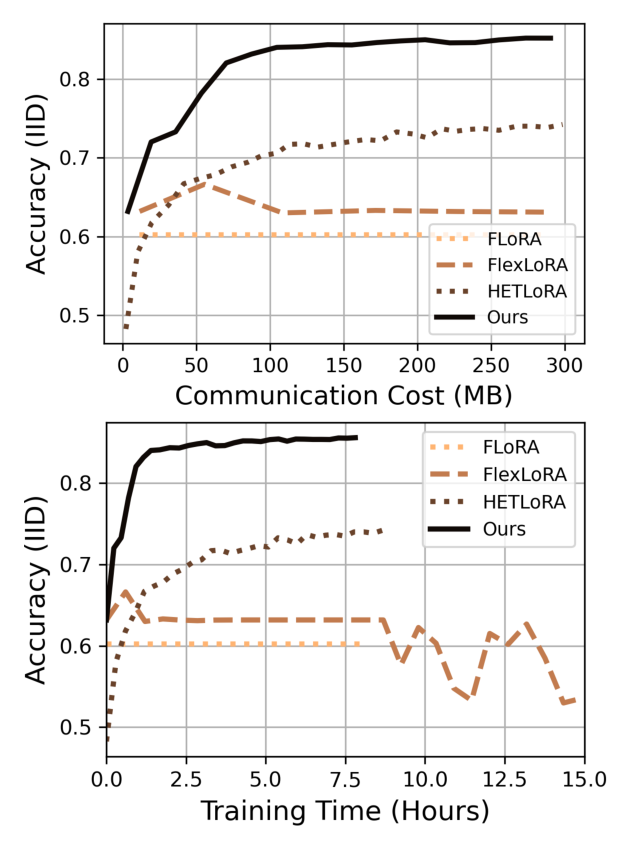
\includegraphics[width=0.95\linewidth]{fig/comp_comm_eff.pdf}
%     \caption{Accuracy over communication cost and training time on QQP dataset.}
%     \label{fig:qqp_comp_comm_eff}
%     % \vspace{-8pt}
% \end{wrapfigure}
% % \end{figure}



\vspace{-10pt}
\subsection{Additional Discussions}\label{subsec:quantitative_analysis}




% \begin{wrapfigure}{r}{0.5\linewidth}\vspace{-20pt}
%     % \centering
%     \begin{subfigure}[b]{0.5\linewidth}
%         \includegraphics[width=\linewidth]{Screenshot 2025-09-24 at 10.13.50 AM.png} \vspace{-5pt}
%         \caption{}
%         \label{fig:adapt}
%     \end{subfigure}
%     % \hfill
%     \begin{subfigure}[b]{0.48\linewidth}
%         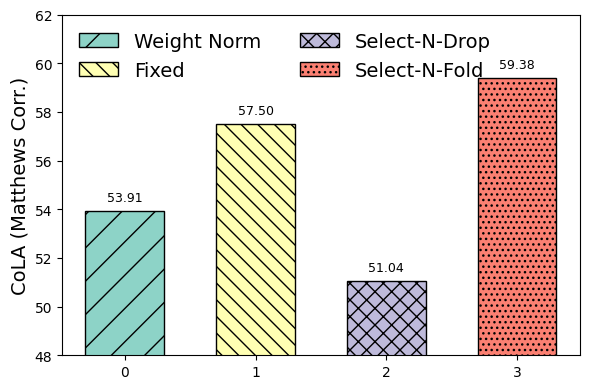
\includegraphics[width=\linewidth]{download.png}
%         \vspace{-5pt}
%         \caption{}
%         \label{fig:select}
%     \end{subfigure}\vspace{-5pt}
%     \caption{(a) Performance of Fed-PLoRA and Fed-PrsLoRA in homogeneous settings. (b) Performance of Select-N-Fold compared with other selection methods.}
% \end{wrapfigure}




\textbf{Adaptability of the PLoRA to Homogeneous Settings and LoRA Variants.} 
\begin{wrapfigure}{r}{0.35\linewidth}
\vspace{-10pt}
\centering
    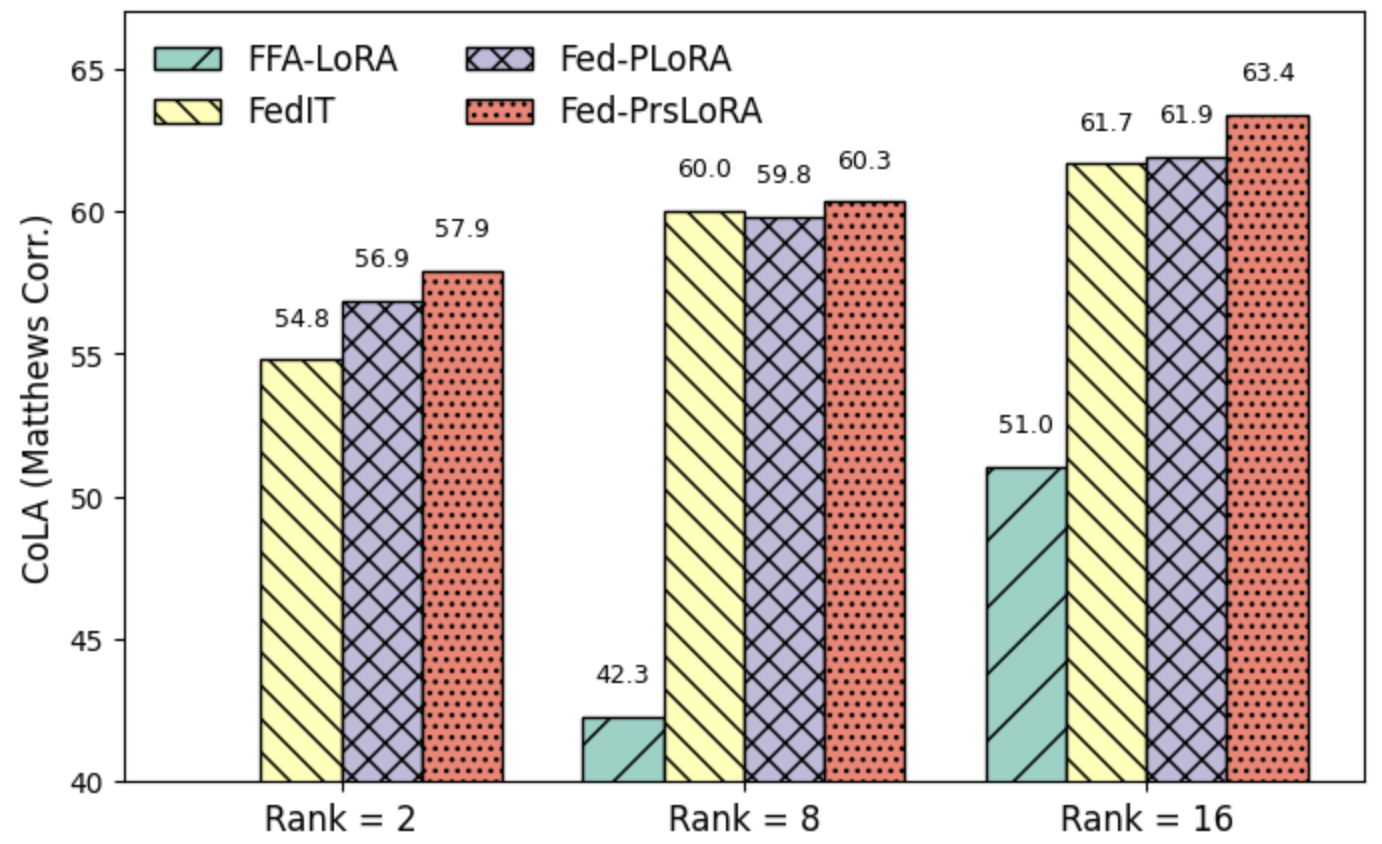
\includegraphics[width=\linewidth]{fed-prslora.png} 
    \vspace{-15pt}
    \caption{Performance of PLoRA and Fed-PrsLoRA in homogeneous settings.} \vspace{-5pt}
    \label{fig:adapt}
    \vspace{-11pt}
\end{wrapfigure}
\begin{wrapfigure}{r}{0.56\linewidth}
\vspace{-28pt}
\centering
    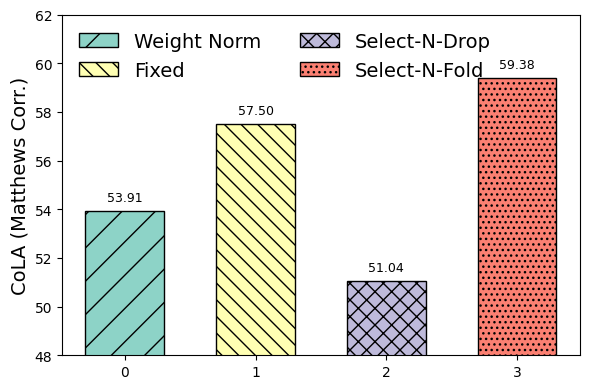
\includegraphics[width=\linewidth]{download.png}
    \vspace{-15pt}
    \caption{Select-N-Fold vs. other selection methods.}
    \vspace{-40pt}
    \label{fig:select}
\end{wrapfigure}
Theoretically, PLoRA achieves the same adaptation effect and parameter efficiency as standard multi-rank LoRA (see Section~\ref{plora}) and can be extended to other LoRA variants. We adapt it to rsLoRA~\cite{kalajdzievski2023rank}, forming Fed-PrsLoRA, and compare with FedIT and another homogeneous method FFA-LoRA~\cite{sun2024improving} (which only shares $B$ matrices). 
We evaluate on IID CoLA dataset, the hardest GLUE task, under homogeneous settings with different ranks. 
From Figure~\ref{fig:adapt}, we observe that Fed-PrsLoRA consistently outperforms Fed-PLoRA, leveraging rsLoRA’s improvements over LoRA. Both methods also achieve substantial gains over FFA-LoRA (e.g., +10.63\% and +10.89\% at rank 16) and in some cases surpass FedIT. This advantage becomes more pronounced as the rank decreases, underscoring the effectiveness of PLoRA’s parallelization in resource-limited settings.


\textbf{Effectiveness of Select-N-Fold.} We also evaluate other strategies for selecting trainable one-rank PLoRA modules in Fed-PLoRA on IID CoLA dataset. We consider: Weight Norm, which picks modules with the largest weight norms; Fixed, which always selects the first $r_i$ modules; and Select-N-Drop, which randomly selects $r_i$ modules like Select-N-Fold but discards the rest. 
As shown in Figure~\ref{fig:select}, both random strategies (Select-N-Drop and Select-N-Fold) outperform the deterministic ones, since randomness ensures that all global PLoRA modules are eventually updated. Select-N-Fold achieves the highest performance by additionally reusing the latest unselected modules during local training. 


\noindent\textbf{Communication and Computational Efficiency.} Figure~\ref{fig:qqp_comp_comm_eff} shows the accuracy of four heterogeneous methods on the IID QQP dataset with respect to communication (uplink and downlink) cost and computation (wall-clock training time) cost. Overall, Fed-PLoRA achieves higher communication efficiency although it incurs additional $R-r_i$ downlink cost compared to others. Both Fed-PLoRA and HETLoRA achieve good computational efficiency as they are lightweight. FlexLoRA incurs substantial computational overhead due to the use of SVD, nearly doubling the training time. A detailed overhead analysis is given in \supplement{Appendix Section~\ref{appendixsec:overhead_analysis}}.

% In Fed-PLoRA, the server transmits all $R$ global one-rank parallel matrix pairs to sampled clients to ensure optimal initialization. Despite this, our method achieves better overall communication efficiency than existing methods. In terms of computational efficiency, FlexLoRA incurs substantial overhead from its server-side SVD operations in each round, nearly doubling the training time. By contrast, Fed-PLoRA reaches the target accuracy faster, offering the best overall training efficiency. A detailed analysis of resource overheads (including communication, computation, and storage) is provided in \supplement{Appendix Section~\ref{appendixsec:overhead_analysis}}


% \subsection{Ablation Studies}

% \subsection{Discussions}
% Due to space constraints, we present detailed discussions on more experimental results under various settings and potential extensions in the \supplement{Appendix}. 
% In \supplement{Appendix Section~\ref{appendixsection:exps}}, we provide more experimental results on GLUE, Dolly-15K, and medical datasets.
% In \supplement{Appendix Section~\ref{appendixsubsection:plora2homo}}, we discuss the adaptability of the PLoRA module to homogeneous rank setting and LoRA variants.
% In \supplement{Appendix Section~\ref{appendixsubsection:selection}}, we provide justification for our rank selection strategy using both experimental results and visualizations.
% In \supplement{Appendix Section~\ref{appendixsubsection:init_agg_observation}}, we provide empirical observations on initialization and aggregation noise.
% In \supplement{Appendix Section~\ref{appendixsubsection:num_ratio}}, we examine the impact of client-related hyperparameters, including the total number of clients, the resource heterogeneity ratio, and client rank combinations.
% In \supplement{Appendix Section~\ref{appendixsubsection:server_hyper}}, we discuss the case under an extreme setting with a large global model rank.
% Additionally, we analyze the effects of the PLoRA module rank and the role of Dropout in \supplement{Appendix Section~\ref{appendixsubsection:plora_rank}} and \supplement{Appendix Section~\ref{appendixsubsection:dropout}}, respectively.
% Finally, in \supplement{Appendix Section~\ref{appendixsubsection:vis_cos_sim}}, we provide additional visualizations of cosine similarities across all transformer layers.

% Due to space limitations, we provide detailed discussions of additional experiments and potential extensions in the \supplement{Appendix}. Specifically, \supplement{Appendix Section~\ref{appendixsection:exps}} reports further results on GLUE, Dolly-15K, and medical datasets. \supplement{Appendix Section~\ref{appendixsubsection:plora2homo}} explores the adaptability of the PLoRA module to homogeneous rank settings and compatibility with LoRA variants. In \supplement{Appendix Section~\ref{appendixsubsection:selection}}, we justify our rank selection strategy using empirical evidence and visualizations. Empirical observations on initialization and aggregation noise are presented in \supplement{Appendix Section~\ref{appendixsubsection:init_agg_observation}}.
% We examine the impact of client-side hyperparameters, such as the total number of clients, the degree of resource heterogeneity, and client rank configurations in \supplement{Appendix Section~\ref{appendixsubsection:num_ratio}}. An extreme setting involving a large global model rank is analyzed in \supplement{Appendix Section~\ref{appendixsubsection:server_hyper}}. The effects of PLoRA rank and Dropout are discussed in \supplement{Appendix Sections~\ref{appendixsubsection:plora_rank}} and~\ref{appendixsubsection:dropout}, respectively. Finally, we include additional visualizations of cosine similarities across transformer layers in \supplement{Appendix Section~\ref{appendixsubsection:vis_cos_sim}}.
\vspace{-10pt}
\section{Related Work}


LoRA-based FFT has recently emerged as a popular paradigm for adapting LLMs while preserving data privacy~\cite{zhang2023towards,babakniya2023slora,sun2024improving,zawad2025fedcust}. Early approaches such as FedIT~\cite{zhang2023towards} and FFA-LoRA~\cite{sun2024improving} combine LoRA with FedAvg or modify update sharing to mitigate aggregation noise, but they assume homogeneous client resources. Other work like FedSA-LoRA~\cite{guo2024selective} explores selective aggregation, yet still under homogeneous settings. 
 \begin{wrapfigure}{r}{0.38\linewidth}
\vspace{-25pt}
\centering
    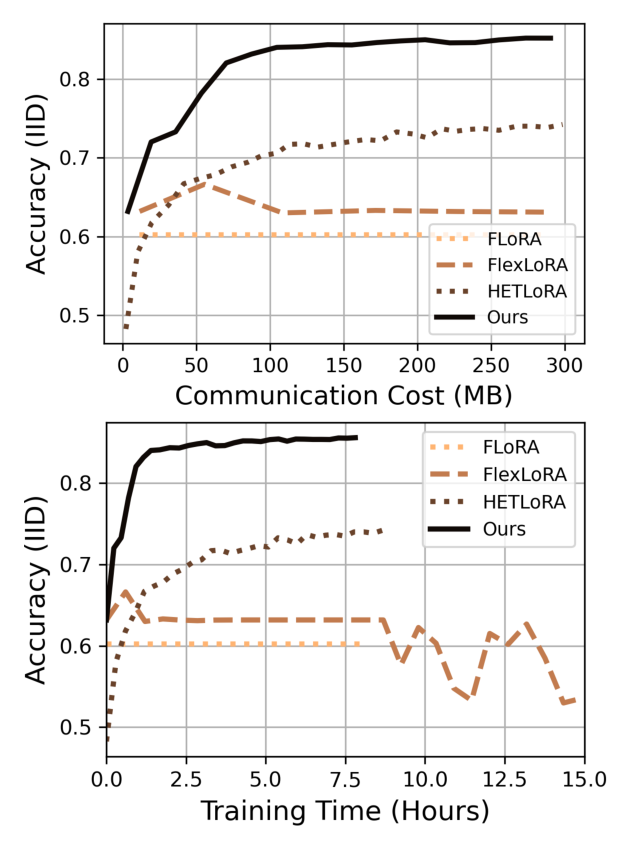
\includegraphics[width=\linewidth]{fig/comp_comm_eff.pdf}
    \vspace{-25pt}
    \caption{Training efficiency of Fed-PLoRA.}
    \vspace{-20pt}
    \label{fig:qqp_comp_comm_eff}
\end{wrapfigure}
To address resource heterogeneity, several methods allow clients to fine-tune with different LoRA ranks. HETLoRA~\cite{cho2024heterogeneous} aggregates heterogeneous updates through zero-padding and truncation, FLoRA~\cite{wangflora} stacks full-weight updates before reinitialization, and FlexLoRA~\cite{bai2024federated} applies SVD-based aggregation with truncation. While effective to some extent, these approaches introduce substantial initialization or aggregation noise, degrading global performance.

The use of multiple parallel LoRA modules has been explored, for enhancing model capacity in centralized training, e.g., Capaboost~\cite{haoboincreasing} and MELoRA~\cite{ren2024melora} rather than addressing the unique challenges of federated settings. In contrast, our work designs PLoRA as a mechanism to mitigate initialization and aggregation noise under heterogeneous FFT. 
% 

Finally, other efficiency-oriented techniques such as quantization~\cite{frantar2022gptq,lin2024awq}, zeroth-order optimization~\cite{xu2024fwdllm,zhang2024revisiting}, and system-level methods like activation checkpointing~\cite{chen2016training} provide complementary directions for resource-efficient training. These are orthogonal to our design and could be combined with Fed-PLoRA in future work. Due to the limited space, we provide a comprehensive literature review in \supplement{Appendix Section~\ref{appendixsection:relatedworks}}.

\section{Conclusion}

In this paper, we introduced Fed-PLoRA, a novel heterogeneous FFT framework designed to tackle the fundamental challenges of initialization and aggregation noise in LoRA-based fine-tuning. By leveraging PLoRA’s parallel one-rank modules together with the Select-N-Fold strategy, Fed-PLoRA aligns client updates more effectively and preserves consistency under resource heterogeneity. We conducted a unified analysis of initialization and aggregation noise of our method, comparing with state-of-the-art heterogeneous LoRA-based FFT methods. 
Through extensive experiments on multiple tasks, we justified the effectiveness of PLoRA and Select-N-Fold and showed that Fed-PLoRA consistently outperforms existing state-of-the-art methods in both accuracy and efficiency. PLoRA’s parallelization design opens new opportunities for integration with other LoRA-like methods, potentially extending its benefits beyond the current framework. In the future, we will work on further reducing the noise that arises during the aggregation of low-rank adaptations and investigating how parallelization can be leveraged to better align model updates under data heterogeneity. %, strengthening both the robustness and scalability of FFT systems.

% In this paper, we conduct a unified analysis of initialization and aggregation noise for SOTA heterogeneous FFT methods. To mitigate the initialization noise and reduce aggregation noise, we introduce Fed-PLoRA, a novel framework that employs parallel, one-rank LoRA modules combined with a novel \textit{Select-N-Fold} strategy. Extensive experiments across diverse LLM fine-tuning tasks demonstrate the effectiveness of our method.

\section*{Acknowledgments}
This work was supported by the National Science Foundation under the Harnessing the Data Revolution for Nevada Fire Science (HDRFS) Seed Grant NSHE-24-37.

\bibliography{main}
\bibliographystyle{iclr2026_conference}


\appendix

% \setcounter{secnumdepth}{2}
% \renewcommand\thesection{\Alph{section}}       % section 编号为 A, B, C...
% \renewcommand\thesubsection{\thesection.\arabic{subsection}}  % subsection 编号为 A.1, B.1...

\newpage

\section*{Appendix}

This appendix presents additional discussions and experimental details to support the main text. The content is organized as follows:

\begin{itemize}
    \item Appendix Section~\ref{appendixsection:codesnippet}: A code snippet illustrating how our method can be easily integrated into existing frameworks{, as well as pseudo-code of Fed-PLoRA.
    }

    % \item {Appendix Section~\ref{appendixsection:pseudocode}: Pseudo-code of Fed-PLoRA.}

    \item Appendix Section~\ref{appendixsection:relatedworks}: Extended literature review on related work.

    \item Appendix Section~\ref{appendixsection:settings}: Detailed description of experimental settings.
        \begin{itemize}
            \item Subsection~\ref{appendixsection:datasets}: Dataset and model descriptions.
            \item Subsection~\ref{appendixsubsection:main_settings}: Settings for the main experiments, including FL configuration and infrastructure.
            \item Subsection~\ref{appendixsubsection:other_settings}: Settings for the experiments in Figure~\ref{fig:motivation} and Figure~\ref{fig:aggregation_noise}.
        \end{itemize}

    \item Appendix Section~\ref{appendixsection:exps}: Additional experimental results.
        \begin{itemize}
            \item Subsection~\ref{appendixsubsection:glue-noniid}: Results on the GLUE benchmark under the non-IID setting.
            \item Subsection~\ref{appendixsubsection:dolly15k}: Results on the Dolly-15K dataset under both IID and non-IID settings.
            \item Subsection~\ref{appendixsubsection:medical}: Results on the Medical Question Answering datasets.
            \item {Subsection~\ref{appendixsubsection:math}: Results on the MATH reasoning datasets.}


            \item Subsection~\ref{appendixsection:ablexps}: Ablation studies.
                \begin{itemize}
                    % \item Subsection~\ref{appendixsubsection:plora2homo}: Adaptability of PLoRA to homogeneous ranks and other LoRA variants.
                    \item Subsection~\ref{appendixsubsection:selection}: Effectiveness of different selection methods for PLoRA modules.
                    \item Subsection~\ref{appendixsubsection:init_agg_observation}: Empirical observations on initialization and aggregation noise.
                    \item Subsection~\ref{appendixsubsection:num_ratio}: Impact of the number of clients, heterogeneity ratio, and local rank per client.
                    % \item Subsection~\ref{appendixsubsection:server_hyper}: Effects of extremely large global model rank.
                    \item Subsection~\ref{appendixsubsection:plora_rank}: Effects of different PLoRA ranks.
                    \item Subsection~\ref{appendixsubsection:dropout}: Effects of Dropout.
                    \item Subsection~\ref{appendixsubsection:vis_cos_sim}: Additional visualizations of cosine similarity across PLoRA modules.
                \end{itemize}
        \end{itemize}
                



    \item Appendix Section~\ref{appendixsec:analysis}: Analysis of initialization and aggregation noise in existing methods.
        \begin{itemize}
            \item Subsection~\ref{appendixsubsection:flora}: Derivations for FLoRA.
            \item Subsection~\ref{appendixsubsection:flexlora}: Derivations for FlexLoRA.
            \item Subsection~\ref{appendixsubsection:hetlora}: Derivations for HETLoRA.
            \item  Subsection~\ref{appendixsubsection:fedplora}: Detailed derivations of the aggregation noise for Fed-PLoRA.
        \end{itemize}

    \item Appendix Section~\ref{appendixsection:additionalstudies}: Additional Studis.
        \begin{itemize}
    
            \item Subsection~\ref{appendixsection:eff_rank_method}: Demonstration of the efficiency of the rank-based method on resource-constrained devices.
            
            \item Subsection~\ref{appendixsec:overhead_analysis}: Theoretical and numerical analysis of the resource overhead for existing methods and Fed-PLoRA.
        \end{itemize}
    
\end{itemize}


\section*{Use of LLM Statement}
For the preparation of this manuscript, AI assistants are utilized to aid in checking grammar, spelling, and punctuation.

\section{Code snippet and pseudo-code}\label{appendixsection:codesnippet}

\begin{codeblock} 
# Implementation
# Just one line of code to apply Parallel One-Rank LoRA in PyTorch.
model = AutoModelForCausalLM.from_pretrained(model_name)
(*@\markDel{- config = LoraConfig(r=8,$\cdots$)}@*)
(*@\markAdd{+ config = PLoraConfig(r=1,NumModule=8,$\cdots$)}@*)
get_peft_model(model, config)
\end{codeblock}

We implement Fed-PLoRA using the Huggingface-style LoRA initialization API (as shown above), making it easy to use by replacing just a single line in the original code.

% \section{Pseudo-code of Fed-PLoRA}\label{appendixsection:pseudocode}
{To better illustrate the proposed method, we present the pseudo-code of Fed-PLoRA as follows.}

\setlength{\textfloatsep}{3pt}
\begin{algorithm}[h]

\caption{{Fed-PLoRA}}\label{algorithm-ours}
\begin{algorithmic}[1]
\REQUIRE Number of communication rounds $T$, global rank $R$, local ranks $\{r_i\}_{i\in[v]}$, pre-trained backbone $\boldsymbol{\Theta}^0$, initial global PLoRA parameters $\boldsymbol{\theta}^0$
\STATE Server sends $\boldsymbol{\Theta}^0$ to all clients
\FOR{$t=1$ to $T$}
    \STATE Server samples a set of clients $\mathcal{S}^t \subseteq [v]$ 
    \STATE Server sends global PLoRA parameters $\boldsymbol{\theta}^{t-1}$ to $i \in \mathcal{S}^t$
    \FOR{each client $i \in \mathcal{S}^t$ \textbf{in parallel}}
        \STATE Randomly sample a subset $\mathcal{K}_i^{t}$ of size $r_i$ from index set $[R]$
        \STATE Initialize local trainable PLoRA modules: $\boldsymbol{\theta}_i^{t-1} \leftarrow \{\boldsymbol{A}_{(j)}^{t-1}, \boldsymbol{B}_{(j)}^{t-1}\;\}_{j \in \mathcal{K}_i^t}$
        \STATE Fold unselected modules into the frozen target weights: $\boldsymbol{\mathcal{W}}_i^{t} \leftarrow \boldsymbol{\mathcal{W}}^{0} + \sum_{j \notin \mathcal{K}_i^{t}} \boldsymbol{B}_{(j)}^{t-1} \boldsymbol{A}_{(j)}^{t-1}$ to obtain the local frozen backbone $\boldsymbol{\Theta}_i^{t}$
        \STATE Obtain new local PLoRA parameters: $\boldsymbol{\theta}_i^{t} \leftarrow \LocalUpdate(\boldsymbol{\theta}_i^{t-1}, D_i, \boldsymbol{\Theta}_i^t)$
    \ENDFOR
    \STATE Rank-wise aggregation of PLoRA modules: $\boldsymbol{\theta}^{t} \leftarrow \Agg\big(\{\boldsymbol{\theta}_i^{t}\}_{i\in\mathcal{S}^t}, \{\mathcal{K}_i^{t}\}_{i\in\mathcal{S}^t}\big)$
    \STATE Update global model: $\boldsymbol{\Phi}_g^{t+1} \leftarrow \{\boldsymbol{\Theta}^0, \boldsymbol{\theta}^{t}\}$
\ENDFOR
\STATE \textbf{return} $\boldsymbol{\Phi}_g^T=\{\boldsymbol{\Theta}^0, \boldsymbol{\theta}^T \}$
\end{algorithmic}
\end{algorithm}

\section{Comprehensive Literature Reviews}\label{appendixsection:relatedworks}

\textbf{Federated LoRA-based Fine-tuning.} The application of FL to LoRA-based fine-tuning of LLMs has become a prominent paradigm, enabling multiple clients to collaboratively adapt models without sharing their raw data~\cite{zhang2023towards, babakniya2023slora, sun2024improving,zhang2024federated}.
Several prior works have investigated this combination:
FedIT~\cite{zhang2023towards} introduces a naive federated fine-tuning method with LoRA and FedAvg, serving as an effective benchmark for further research. 
% SLoRA~\cite{babakniya2023slora} proposes a two-stage training framework, initiating with sparse full fine-tuning locally for several rounds before utilizing these fine-tuned weights to initialize LoRA modules. 
FFA-LoRA~\cite{sun2024improving} introduces a strategy of freezing the LoRA $\mathbf{A}$ matrix during local training to help mitigate aggregation noise at the server. Furthermore, FedSA-LoRA~\cite{guo2024selective} explores selective aggregation for a personalized FL system, which is designed to only share the $\mathbf{A}$ matrix with the server for aggregation, due to its specific role in learning general knowledge. However, these methods assume homogeneous client resources, which often do not align with the varied resources present in practical FL systems.

\noindent\textbf{Federated Fine-Tuning with Heterogeneous LoRA Ranks.} Resource heterogeneity remains a significant challenge in federated fine-tuning. To address this, HETLoRA~\cite{cho2024heterogeneous} allows clients to train with different LoRA ranks based on their capacity. For aggregation, local model modules from smaller ranks are zero-padded, and the resulting global LoRA module is subsequently truncated for client LoRA module initialization. However, this process introduces both initialization and aggregation noise due to the limited LoRA rank.
FLoRA~\cite{wangflora} employs a stacking-based aggregation method, which is designed to accurately aggregate LoRA module updates from clients with heterogeneous ranks in a full-weight space. While this aims for optimal aggregation, FLoRA then applies this update to the client's target module, and the trainable LoRA modules for the next round are typically initialized from scratch, thereby incurring significant initialization noise.
FlexLoRA~\cite{bai2024federated} utilizes SVD during aggregation, and then initializes LoRA modules for clients with varying ranks by truncation. These processes lead to both aggregation and initialization noise.

\noindent\textbf{Parallel Low-Rank Adaptation {and Sparse LoRA Fine-Tuning.}} The concept of employing multiple parallel LoRA modules has been investigated primarily for enhancing model capacity. For instance, Capaboost~\cite{haoboincreasing} applies different random masks to a single large rank LoRA module during training, effectively simulating an ensemble of parallel LoRA modules to increase model capacity without incurring additional parameter costs. MELoRA~\cite{ren2024melora} adopts a group of mini LoRA modules to obtain sparse $\mathbf{A}$ and $\mathbf{B}$ matrices. They claim that each LoRA module is designed to capture different features. 
% While t
These approaches leverage the parallelism of the LoRA module for capacity scaling.
% , their primary focus is not typically on the intricacies of the federated learning process. 
In contrast, our framework introduces parallel one-rank LoRA modules specifically as a way to improve initialization and aggregation within the FL system.

{
Another related line of work~\cite{zhou2021learning,zhang2022learning} studies sparse LoRA fine-tuning, where only a subset of LoRA rows is updated while the remaining rows are simply frozen. In principle, such sparsification yields similar training dynamics on the active rows, since the inactive rows receive zero gradients. However, this design has several system-level limitations. First, the frozen rows must still be stored in GPU memory and participate in the forward pass, which increases activation storage and peak memory consumption compared with physically removing these rows. Second, the resulting sparsity pattern is typically unstructured: it does not match the $N\!:\!M$ structured sparsity patterns required by modern accelerators (for example, the 2:4 pattern used by NVIDIA A100 sparse tensor cores~\cite{zhou2021learning}). As a result, simply freezing $R - r_i$ out of $R$ rows cannot exploit hardware sparsity support or lead to real speedups. In contrast, Fed-PLoRA folds unused one-rank modules into the backbone weights, preserving the same effective training behavior on active ranks while avoiding extra computation and memory overhead, which makes it more suitable for large-scale federated deployment.
}

\noindent\textbf{Other Resource-Efficient Fine-Tuning Pathways.} 
Quantization is a widely studied technique for improving inference efficiency by reducing the precision of model weights and activations. Common methods include post-training quantization (PTQ), quantization-aware training (QAT), and activation quantization.
PTQ~\cite{frantar2022gptq,lin2024awq,xiao2023smoothquant} applies quantization to a pretrained model without modifying its training process. It is simple and efficient but may lead to noticeable accuracy degradation, especially for low-bit quantization or in sensitive tasks. 
QAT~\cite{nagel2022overcoming} is particularly focused on preserving inference-time accuracy by simulating low-precision operations (e.g., 8-bit or 4-bit) during training through the insertion of fake quantization nodes in the computation graph, allowing the model to adapt to quantization effects. However, QAT typically targets deployment-time efficiency and does not substantially reduce training-time memory or compute costs.
Activation quantization~\cite{choi2018pact} focuses on reducing the bit-width of intermediate activations in addition to weights. While this offers additional memory savings during training, it also introduces additional quantization noise and quantization and de-quantization costs with extra computation. This can make training more unstable and often requires careful calibration to preserve performance.

Zeroth-order optimization~\cite{xu2024fwdllm} reduces memory usage by avoiding explicit gradient computation. Since it does not require backpropagation, it eliminates the need to store intermediate activations during the forward pass. However, this benefit comes with notable trade-offs: zeroth-order methods typically require many more function evaluations (i.e., higher query complexity) to estimate gradients indirectly, and the resulting gradient estimates tend to be noisier. These factors can significantly slow down convergence, particularly for large, high-dimensional models like LLMs, where accurate and efficient gradient information is crucial for effective training~\cite{zhang2024revisiting}.

In addition to algorithmic approaches, several system-level engineering strategies have been developed to address the memory and compute bottlenecks of large model fine-tuning. These methods aim to optimize training pipelines without modifying model architectures or learning objectives. For example, activation checkpointing~\cite{chen2016training} reduces GPU memory usage by storing only a subset of activations during the forward pass and recomputing the rest during backpropagation. While it enables training deeper models under tight memory budgets, the trade-off is increased computational overhead due to repeated forward computations. This may lengthen training time significantly, especially in models with expensive forward passes.

All the above techniques are orthogonal and potentially complementary to our approach and could be integrated in specific scenarios. However, in the context of our work, these comparisons are less directly relevant to serve as comparisons. We will consider exploring such combinations in our future work.




\section{Experimental Settings}\label{appendixsection:settings}

\subsection{Datasets and Models}\label{appendixsection:datasets}
\textbf{General Language Understanding Task.}
For evaluating general language understanding proficiency, we follow Hao et al.~\cite{haoboincreasing} that utilize six well-established datasets from the General Language Understanding Evaluation (GLUE) benchmark, as detailed by Wang et al.~\cite{wang2018glue}. Specifically, the tasks included the Corpus of Linguistic Acceptability (CoLA), the Stanford Sentiment Treebank (SST-2), the Microsoft Research Paraphrase Corpus (MRPC), the Quora Question Pairs (QQP) dataset, Question NLI (QNLI), and the Recognizing Textual Entailment (RTE) dataset. Across all these GLUE tasks, the BERT-base model, introduced by Devlin et al.~\cite{devlin2019bert}, is employed as the foundational pre-trained language model.

\noindent\textbf{General Instruction Following Task.}
To assess the framework's performance on tasks requiring general instruction following, we benchmark on two prominent datasets, following the approach of Bai et al.~\cite{bai2024federated}. The first dataset is Natural Instructions (NI), a large-scale collection of diverse NLP tasks structured as instructions, developed by Wang et al.~\cite{wang2022super}. For this dataset, we utilized a Llama-1B model, with weights sourced from the Data-Juicer project by Chen et al.~\cite{chen2024data}. The second dataset is Dolly-15K, an open-source dataset of instruction-followed records created by Databricks~\cite{conover2023free}, for which the OPT-1.3B model from Zhang et al.~\cite{zhang2022opt} is employed.

\noindent\textbf{Domain-Specific Tasks.}
We further extend our evaluation to domain-specific applications, focusing on the challenging medical and financial domains. \textbf{Medical Domain:} Adhering to the experimental design outlined by Ye et al.~\cite{ye2024openfedllm} and Flower~\cite{flower2024flowertune}, we utilize the MedAlpaca dataset, curated by Han et al.~\cite{han2023medalpaca}, for the training phase of our medical domain tasks. The framework's effectiveness is then evaluated on four widely recognized medical question answering benchmarks: PubMedQA by Jin et al.~\cite{jin2019pubmedqa}, MedMCQA by Pal et al.~\cite{pal2022medmcqa}, MedQA (USMLE-style questions) also by Jin et al.~\cite{jin2021disease}, and CareQA~\cite{arias2025automatic}. For these demanding medical tasks, we employ the Mistral-7B-v0.3 model~\cite{mistral7b2023}, leveraging QLoRA for 4-bit precision fine-tuning, as proposed by Dettmers et al.~\cite{dettmers2023qlora}. \textbf{Financial Domain:} For the financial domain, training is conducted on a financial sentiment analysis dataset derived from the FinGPT project by Yang et al.~\cite{fingpt2023dataset}. Evaluation is performed on three established financial NLP benchmarks: the Financial PhraseBank (FPB) by Malo et al.~\cite{malo2014good}, the Financial Sentiment Analysis on News Headlines (FIQA) dataset by Maia et al.~\cite{maia201818}, and the Twitter Financial News Sentiment (TFNS) dataset~\cite{twitter_financial_news_2022}. These financial experiments are carried out using the Llama-3.1-8B model from Meta~\cite{meta2024llama31}, also fine-tuned with QLoRA in 4-bit precision.

{\noindent\textbf{Reasoning Tasks.} We additionally evaluate our framework on mathematical reasoning, using the MATH benchmark introduced by Hendrycks et al.~\cite{hendrycksmath2021}. This dataset contains 12,500 competition-style math problems, each tagged by subject (algebra, counting and probability, geometry, number theory, etc.) and difficulty level from 1 to 5. Unlike standard word-problem benchmarks, MATH emphasizes multi-step deduction and symbolic manipulation rather than direct pattern matching, making it a strong stress test for federated parameter-efficient tuning. Every problem includes a full step-by-step solution, enabling training signals beyond final answer supervision. For these math tasks, we employ the Qwen3-4B-Instruct-2507 model, leveraging QLoRA for 4-bit precision fine-tuning, similar to the previous model settings.
}


\noindent\textbf{Data Heterogeneity.}
To evaluate the performance under diverse data distributions, we specifically assess task heterogeneity using the Natural Instructions, Dolly-15K, and GLUE datasets, as they naturally consist of varied instruction-based or classification-based tasks. We apply both pathological and Dirichlet partitioning methods: the pathological method skews the number of tasks or label categories available to each client, while the Dirichlet method primarily controls the number of samples per client. For Natural Instructions, we use an extreme case where each client is assigned 20 out of 612 tasks; for Dolly-15K, each client receives data from only 1 out of 7 tasks. In the GLUE setup, we apply Dirichlet partitioning with $\alpha=0.01$, resulting in a highly imbalanced distribution of samples across clients. For all other datasets, we adopt IID partitioning.


\subsection{Main Result Settings}\label{appendixsubsection:main_settings}




\begin{table*}[h]
  \centering
  \caption{FL settings for all experiments.}
  \renewcommand{\arraystretch}{1.2} 
  \scalebox{0.50}{
    \begin{tabular}{c|cccccc}
    \toprule[1.2pt]
    \textbf{Dataset/Configuration} & \textbf{Model} & \textbf{LoRA} & \textbf{Client} & \textbf{Training Round} & \textbf{Learning Rate} & \textbf{batch size} \\
    \midrule
    \textbf{CoLA} & BERT-base & rank=1/4/16, lora\_alpha=1/4/16, target\_modules=[``query'', ``value''] & 100 (10\%) & 200     & 0.001 & 16     \\
    \textbf{SST-2} & BERT-base & rank=1/4/16, lora\_alpha=1/4/16, target\_modules=[``query'', ``value''] & 100 (10\%) & 45     & 0.001 & 16     \\
    \textbf{MRPC} & BERT-base & rank=1/4/16, lora\_alpha=1/4/16, target\_modules=[``query'', ``value''] & 100 (10\%) & 150     & 0.001 & 16     \\
    \textbf{QQP} & BERT-base & rank=1/4/16, lora\_alpha=1/4/16, target\_modules=[``query'', ``value''] & 100 (10\%) & 150     & 0.001 & 16     \\
    \textbf{QNLI} & BERT-base & rank=1/4/16, lora\_alpha=1/4/16, target\_modules=[``query'', ``value''] & 100 (10\%) & 50     & 0.001 & 16     \\
    \textbf{RTE} & BERT-base & rank=1/4/16, lora\_alpha=1/4/16, target\_modules=[``query'', ``value''] & 100 (10\%) & 150     & 0.001 & 16     \\
    \textbf{Natural Instruction} & Llama (Data-Juicer-1B) & rank=1/8/16, lora\_alpha=1/8/16, target\_modules=[``q\_proj'', ``v\_proj''] & 50 (10\%) & 25     & 0.00001 & 4     \\
    \textbf{Dolly-15K} & OPT-1.3B & rank=1/8/32, lora\_alpha=1/8/32, target\_modules=[``q\_proj'', ``v\_proj''] & 50 (10\%) & 25    & 0.00001 & 4     \\
    \textbf{Medical} & Mistral-7B-v0.3 & rank=1/2/8, lora\_alpha=1/2/8, target\_modules=[``q\_proj'', ``v\_proj''] & 50 (10\%) & 50    & 0.00005 & 4     \\
    \textbf{Finance} & Llama-3.1-8B & rank=1/2/8, lora\_alpha=1/2/8, target\_modules=[``q\_proj'', ``v\_proj''] & 50 (10\%) & 15    & 0.00005 & 4     \\
    {\textbf{MATH}} & {Qwen3-4B-Instruct-2507} & {rank=1/2/8, lora\_alpha=1/2/8, target\_modules=[``q\_proj'', ``v\_proj'']} & {50 (10\%)} & {15}    & {0.00005} & {4}     \\
    \bottomrule[1.2pt]
    \end{tabular}%
    }
  \label{tab:appendix-fl-settings}%
\end{table*}%

\noindent\textbf{FL Settings.} As shown in Table~\ref{tab:appendix-fl-settings}, the FL configurations for all experiments are comprehensively detailed in Table~\ref{tab:appendix-fl-settings}. This table outlines the specific models, LoRA parameters, client setups, and training hyperparameters employed for each dataset.

For the GLUE benchmark tasks (CoLA, SST-2, MRPC, QQP, QNLI, and RTE), the BERT-base model is utilized. The heterogeneous ranks are set using $R=16, r_m=4$. 
% LoRA is applied with heterogeneous ranks of $(1, 4, 16)$, and corresponding \texttt{lora\_alpha} values, targeting the \texttt{"query"} and \texttt{"value"} modules. 
These experiments involve 100 clients. 
%
Instruction fine-tuning tasks on Natural Instruction and Dolly-15K employed Llama (Data-Juicer-1B) and OPT-1.3B models, respectively. For Natural Instruction, $R=16$ and $ r_m=8$, while for Dolly-15K, $R=16$ and $ r_m=8$. 
%, with \texttt{lora\_alpha} values equal to these ranks. In both cases, LoRA targets the \texttt{"q\_proj"} and \texttt{"v\_proj"} modules. 
These setups use 50 clients. 
%
Domain-specific experiments on Medical and Finance datasets also involve 50 clients. Medical tasks use Mistral-7B-v0.3, Finance tasks use Llama-3.1-8B, and both have $R=16$ and $ r_m=2$. {For mathematical reasoning, we further evaluate on the MATH dataset using Qwen3-4B-Instruct-2507 under the same federated client setup.} All experiments sample 10\% of clients uniformly at random per round.  % Both Medical and Finance experiments set \texttt{lora\_alpha} to match the ranks and targeted \texttt{"q\_proj"} and \texttt{"v\_proj"} modules.


Across these diverse setups, the number of training rounds was task-specific, varying from 15 to 200, as detailed in Table~\ref{tab:appendix-fl-settings}. Learning rates are selected for each task group after evaluating a common search space of \{0.005, 0.001, 0.0005, 0.0001, 0.00005, 0.00001\}; specifically, GLUE tasks utilize a learning rate of 0.001, Natural Instruction and Dolly-15K tasks are trained with 0.00001, and both {Medical, Finance, and MATH} experiments employ a learning rate of 0.00005. Batch sizes are also tailored: 16 for GLUE tasks, 4 for instruction fine-tuning, and 4 for the domain-specific experiments. 

\textit{Justification heterogeneous rank settings:} We empirically evaluate performance across a wide range of LoRA ranks \{1, 2, 4, 8, 16, 32, 64\}. For the highest-resource clients, we select the largest rank that does not lead to overparameterization, following standard practice in FL to ensure a balance between model capacity and resource capacity. For clients with mid-level resources, we adopt middle ranks so that the average rank does not excced the half of the highest rank, reflecting that majoraty of the clients have low resources. 

\textit{Justification for rank settings:} In homogeneous settings, we evaluate LoRA ranks \{1, 2, 4, 8, 16, 32, 64\} to identify the optimal rank. In heterogeneous settings, high-resource clients are assigned this optimal rank to avoid over-parameterization while maintaining a balance between model capacity and device constraints. Low-resource clients are fixed at rank 1. Mid-resource clients are assigned intermediate ranks such that the average rank does not exceed half of the maximum, reflecting the realistic case where most clients are resource-limited. 


We evaluate performance across a broad range of LoRA ranks \{1, 2, 4, 8, 16, 32, 64\} in homogeneous settings and identify the best rank. For high-resource clients in heterogeneous settings, we assign the best rank that avoids over-parameterization, ensuring a balance between model capacity and device constraints. For mid-resource clients, we choose intermediate ranks such that the average rank does not exceed half of the maximum rank, reflecting the realistic scenario where most clients have limited resources.


%This design ensures that the rank allocation reflects practical deployment considerations.

\noindent\textbf{Implementation Details.}
Our framework was implemented using PyTorch version 2.6.0 (built with CUDA 12.4 support). Key libraries included Hugging Face \texttt{transformers} version 4.51.3, \texttt{datasets} version 3.6.0, and \texttt{peft} version 0.9.0 for LoRA and QLoRA functionalities. Experiments were conducted using CUDA 12.4. All experiments were carried out on a server equipped with an AMD EPYC 7763 64-Core Processor, 1.0~TB of system RAM, and 8~$\times$~NVIDIA RTX A6000 GPUs. The total GPU hours for running all the experiments are over 5,000.


\subsection{Other Experimental Settings}\label{appendixsubsection:other_settings}

% we report settings for experiments in Figure~\ref{fig:motivation} and  Figure~\ref{fig:aggregation_noise}.

The experiments illustrated in Figure~\ref{fig:motivation} are conducted on the QQP, MRPC, and RTE datasets using a BERT-based model. A key aspect of this setup is the use of a homogeneous LoRA rank across all clients (i.e., every client uses the same rank). Two distinct homogeneous rank configurations are evaluated: a 'Large Rank' setup with a uniform rank of 16 per client, and a 'Small Rank' setup with a uniform rank of 1 per client. These FL experiments involved a total of 100 clients, with 10\% of clients participating in each training round. The training is conducted for a total of 150 rounds.
%
In Figure~\ref{fig:aggregation_noise}, we report the average cosine similarities calculated for LoRA $\mathbf{A}$ matrices on the Query target module of Layer 1. These calculations are based on experiments performed on the RTE dataset, with a non-IID data distribution achieved by assigning data from only one category to each client.


\section{Additional Experimental Results}\label{appendixsection:exps}



\subsection{Results on non-IID GLUE Dataset}\label{appendixsubsection:glue-noniid}

\begin{table*}[h]
  \centering
  \caption{Evaluation results on GLUE datasets under a non-IID setting (Dirichlet $\alpha=0.01$).}
  \renewcommand{\arraystretch}{1.2} 
  % \setlength{\tabcolsep}{4pt}       
  % {\scriptsize
  \resizebox{\textwidth}{!}{%
  % \scalebox{0.85}{
    \begin{tabular}{c|c|c|cccccc|c}
      \toprule[1.4pt]
      \multicolumn{3}{c|}{\multirow{2}{*}{\textbf{Method}}}
        & \textbf{CoLA} & \textbf{SST-2} & \textbf{MRPC} & \textbf{QQP}
        & \textbf{QNLI} & \textbf{RTE}  &\multirow{2}{*}{\textbf{Avg}}\\
      \multicolumn{3}{c|}{}
        & \textbf{Matthews Corr.} & \textbf{Acc.}
        & \textbf{Acc.} & \textbf{Acc.} & \textbf{Acc.} & \textbf{Acc.} \\
      \midrule
        \multicolumn{3}{c|}{{{Untuned Model}}}
          & {$1.20$}
          & {$49.08$}
          & {$31.61$}
          & {$63.09$}
          & {$49.95$}
          & {$52.70$}
          & {$41.27$} \\
      \midrule
      \multicolumn{2}{c|}{\multirow{2}{*}{{\textbf{Homogeneous}}}}
        & FedIT (Rank=$R$)
          & $56.27$
          & $90.25$
          & $85.29$
          & $87.07$
          & $87.07$
          & $64.62$  
          & $78.28$\\
      \multicolumn{2}{c|}{} 
        & FedIT (Rank=$R/2$)
          & $51.80$
          & $90.25$
          & $79.31$
          & $84.23$
          & $88.01$
          & $61.42$
          & $75.67$\\
      \midrule
      \multicolumn{2}{c|}{\multirow{4}{*}{\shortstack{\textbf{Heterogeneous}\\$R=16$\\{Avg Rank=7}}}}
        & FLoRA
          & $-2.07$
          & $88.97$
          & $68.38$
          & $38.75$
          & $47.37$
          & $47.29$ 
          & $48.18$\\
      \multicolumn{2}{c|}{} 
        & FlexLoRA
          & $38.51$
          & $90.25$
          & $68.39$
          & $79.91$
          & $70.98$
          & $53.79$ 
          &$66.97$\\
      \multicolumn{2}{c|}{} 
        & HETLoRA
          & $40.08$
          & $89.97$
          & $76.35$
          & $81.71$
          & $85.96$
          & $58.12$
          & $72.03$\\
      \multicolumn{2}{c|}{} 
        & \textbf{Fed-PLoRA}
          & \boldmath{$52.33$}
          & \boldmath{$90.71$}
          & \boldmath{$79.65$}
          & \boldmath{$84.79$}
          & \boldmath{$88.01$}
          & \boldmath{$61.01$} 
          & \boldmath{$76.08$}\\
      \bottomrule[1.4pt]
    \end{tabular}%
  }% end resizebox
  % }% end scriptsize
  \label{tab:gluenoniid}
  % \vspace{-10pt}
\end{table*}

Table~\ref{tab:gluenoniid} presents evaluation results on the GLUE dataset under a non-IID setting, where client data distributions are skewed using a Dirichlet distribution with $\alpha=0.01$, representing a highly imbalanced and extreme case. In this challenging scenario, our method Fed-PLoRA consistently outperforms all baselines. Compared to FLoRA, Fed-PLoRA yields substantial gains of +54.40\% on CoLA and +11.27\% on MRPC, underscoring the limitations of FLoRA’s random initialization and emphasizing the benefit of a more carefully designed initialization strategy in our method.
Compared to FlexLoRA, Fed-PLoRA achieves a notable improvement of +17.03\% on QNLI and +0.46\% on SST-2. Although FlexLoRA leverages SVD to derive representative low-rank matrices, it remains susceptible to information loss, which can lead to significant initialization and aggregation noise, especially when some clients operate with much lower ranks than the global configuration and under non-IID cases.
When compared to HETLoRA, Fed-PLoRA improves performance by +3.08\% on QQP and +2.89\% on RTE. These gains come from Fed-PLoRA’s more effective handling of initialization and aggregation noise, which HETLoRA introduces through zero-padding and rank truncation.
Furthermore, Fed-PLoRA surpasses FedIT with a fixed rank of 8 by an average of +0.41\%, despite using a lower average rank of 7. This demonstrates the efficiency and adaptability of our approach that incorporate all resource-constrained clients into training with zero initialization noise and low aggregation noise.

\subsection{Results on Dolly-15K Dataset}\label{appendixsubsection:dolly15k}


\begin{table}[h]
  \centering
  \caption{Evaluation results on IID and non-IID Dolly-15K datasets with OPT-1.3B model.}
  \renewcommand{\arraystretch}{1.2} 
  \scalebox{0.88}{
  \begin{tabular}{c|c|c|cc}
    \toprule[1.2pt]
    \multicolumn{3}{c|}{\multirow{2}{*}{\textbf{Method}}} & \multicolumn{2}{c}{\textbf{Dolly-15K (Rouge-L)}} \\
    \multicolumn{3}{c|}{} & \textbf{IID} & \textbf{non-IID} \\
        \midrule
    \multicolumn{3}{c|}{{{Untuned Model}}}
          & \multicolumn{2}{c}{{$40.02$}}  \\\midrule
    \multicolumn{2}{c|}{\multirow{2}{*}{{\textbf{Homogeneous}}}}
    % &{FedIT (Rank=32)}  & $60.06^{+0.01}_{-0.01}$ & $59.34^{+0.03}_{-0.05}$ \\
    &{FedIT (Rank=$R$)}  & $60.05$ & $59.37$ \\
    \multicolumn{2}{c|}{} &{FedIT (Rank=$R/2$)} &$59.75$ &$59.07$ \\
    \midrule
    \multicolumn{2}{c|}{\multirow{4}{*}{\shortstack{\textbf{Heterogeneous} \\ {$R=32$} \\ {Avg Rank=13}}}} 
      % & FLoRA & $40.01^{+0}_{-0}$ & $40.01^{+0}_{-0}$ \\
      & FLoRA & $40.01$ & $40.01$ \\
    % \multicolumn{2}{c|}{} & FlexLoRA & $57.39^{+0.02}_{-0.03}$  &$51.06^{+6.04}_{-3.79}$  \\
    \multicolumn{2}{c|}{} & FlexLoRA & $57.40$  &$48.82$  \\
    % \multicolumn{2}{c|}{} & HETLoRA & $58.27^{+1.11}_{-0.60}$ & $57.68^{+0.68}_{-0.62}$ \\
    \multicolumn{2}{c|}{} & HETLoRA & $59.38$ & $58.36$ \\
    % \multicolumn{2}{c|}{} & \textbf{Fed-PLoRA} & \boldmath{$60.05^{+0.02}_{-0.03}$} & \boldmath{$59.66^{+0.03}_{-0.01}$} \\
    \multicolumn{2}{c|}{} & \textbf{Fed-PLoRA} & \boldmath{$60.07$} & \boldmath{$59.69$} \\
    \bottomrule[1.2pt]
  \end{tabular}
  }
  \label{tab:dolly15k_rougel}
    % \vspace{-8pt}
\end{table}


% \textbf{Results on Dolly-15K.} 
Table~\ref{tab:dolly15k_rougel} presents the main results on the Dolly-15K dataset. We report Rouge-L scores of the fine-tuned global model under both IID and non-IID settings, where the non-IID scenario is simulated by assigning each client data from only 1 out of 7 distinct tasks. Our method, Fed-PLoRA, consistently outperforms all baseline approaches under both data and resource heterogeneity. Notably, Fed-PLoRA surpasses FlexLoRA in the non-IID setting by a large margin of +10.87\%, highlighting the critical impact of initialization noise in federated fine-tuning. Moreover, Fed-PLoRA even outperforms the homogeneous case with a full rank $32$, achieving gains of +0.02\% and +0.32\% under IID and non-IID conditions, respectively. This suggests that our parallel one-rank LoRA modules offer greater flexibility than conventional high-rank LoRA, and can potentially lead to better overall performance. These results further demonstrate the effectiveness of Fed-PLoRA in mitigating initialization and aggregation noise via its parallelized design.

\subsection{Results on Medical Datasets}\label{appendixsubsection:medical}

\begin{table*}[h]
  \centering
  \caption{Evaluation results on medical datasets with Mistral-7B-v0.3 model.}
  \renewcommand{\arraystretch}{1.2} 
  \scalebox{0.88}{
  \begin{tabular}{c|c|c|cccc|c}
    \toprule[1.5pt]
    \multicolumn{3}{c|}{{\textbf{Method}}} & \textbf{PubMedQA} & \textbf{MedMcQA} & \textbf{MedQA} & \textbf{CareQA} &  {\textbf{Avg}} \\
    \midrule
    \multicolumn{3}{c|}{{{Untuned Model}}}
      & {$55.77$}
      & {$38.43$}
      & {$40.92$}
      & {$41.28$}
      & {$44.10$} \\
    \midrule
    \multicolumn{2}{c|}{\multirow{2}{*}{{\textbf{Homogeneous}}}}
    & FedIT (Rank=$R$)  
    % &$69.13^{+1.47}_{-0.73}$ &$41.23^{+0.12}_{-0.07}$ &$45.79^{+0.40}_{-0.31}$ &$47.46^{+0.37}_{-0.25}$ \\
    &$70.60$ &$41.16$ &$46.19$ &$47.35$ &$51.32$\\
    \multicolumn{2}{c|}{} 
        & FedIT (Rank=$R/2$)
          &$68.60$
          &$41.19$
          &$46.19$
          &$46.55$ %
          &$50.63$\\
    \midrule
    \multicolumn{2}{c|}{\multirow{4}{*}{\shortstack{\textbf{Heterogeneous} \\ $R=8$ \\ {Avg Rank=3}}}} 
      & FLoRA    
      % &$55.80^{+0}_{-0}$ &$40.26^{+0.04}_{-0.01}$ &$45.70^{+0.01}_{-0.01}$ &$46.10^{+0.01}_{-0.02}$ \\
      &$55.80$ &$40.30$ &$45.70$ &$46.10$ &$46.98$\\
    \multicolumn{2}{c|}{} 
    & FlexLoRA 
      % &$60.27^{+2.33}_{-1.87}$ &$41.06^{+0.13}_{-0.23}$ &\boldmath{$46.05^{+0.21}_{-0.26}$} &$46.67^{+0.59}_{-0.44}$  \\
      &$58.40$ &$41.16$ &\boldmath{$46.26$} &$46.26$  &$48.02$\\
    \multicolumn{2}{c|}{} 
    & HETLoRA 
      % &$67.40^{+2.40}_{-2.60}$ &$41.14^{+0.09}_{-0.17}$ &$46.37^{+0.21}_{-0.11}$ &$46.14^{+0.01}_{-0.04}$  \\
      &$69.80$ &$41.23$ &\boldmath{$46.26$} &$46.10$ &$50.85$ \\
    \multicolumn{2}{c|}{} 
    & \textbf{Fed-PLoRA} 
      &\boldmath{$70.20$} &\boldmath{$41.50$} &$46.11$ &\boldmath{$46.85$}  &\boldmath{$51.16$}\\
    \bottomrule[1.5pt]
  \end{tabular}
  }
  \label{tab:medical}
  % \vspace{-10pt}
\end{table*}

% \textbf{Results on Medical and Financial Datasets.} 
Table~\ref{tab:medical} presents the main results (in accuracy) on medical and financial datasets. It is noteworthy that due to the inherent capabilities of the LLMs employed and the potential domain shift between the training and test sets, the observed performance gaps among different federated methods remain relatively small. Fed-PLoRA demonstrates improvements over FLoRA, achieving accuracy gains of +14.40\% on PubMedQA, +1.20\% on MedMcQA, +0.75\% on CareQA, +12.29\% on FPB, and +13.15\% on TFNS. However, when compared to FlexLoRA and HETLoRA on the MedQA dataset and to FLoRA on the FIQA dataset, our method shows slight accuracy drops. This may be attributed to the nature of these domain-specific instruction fine-tuning tasks with large LLMs requiring only a small LoRA rank. In such scenarios, the initialization noise in FlexLoRA and HETLoRA can be relatively small.

{
\subsection{Results on MATH Datasets}\label{appendixsubsection:math}

\begin{table*}[h]

  \centering
  \caption{{Evaluation of Qwen3-4B-A3B-Instruct-2507 on MATH datasets.}}
  \renewcommand{\arraystretch}{1.20}
  \scalebox{0.59}{
  \begin{tabular}{c|c|c|ccccccc|c}
    \toprule[1.5pt]
    \multicolumn{3}{c|}{\textbf{Method}} 
      & \textbf{Algebra} 
      & \textbf{Counting\&Prob.} 
      & \textbf{Geometry} 
      & \textbf{Inter. Algebra} 
      & \textbf{Number Theory} 
      & \textbf{PreAlgebra} 
      & \textbf{PreCalculus}
      & \textbf{Avg} \\
    \midrule
    
    % ================= Homogeneous=================
    \multicolumn{3}{c|}{\textbf{Untuned}} 
      & 12.38 & 5.90 & 3.75 & 1.32 & 5.74 & 15.61 & 4.57 & 7.94 \\
    \midrule
    \multicolumn{2}{c|}{\multirow{2}{*}{\textbf{Homogeneous}}}
      & FedIT (Rank=$R$)
          & 42.20 & 26.79 & 19.20 & 13.73 & 26.11 & 42.93 & 10.98 & 28.38 \\
    \multicolumn{2}{c|}{}
      & FedIT (Rank=$R/2$)
          & 36.47 & 22.57 & 16.70 & 11.62 & 21.48 & 37.08 & 12.27 & 24.62 \\
    \midrule
    
    % ================= Heterogeneous =================
    \multicolumn{2}{c|}{\multirow{4}{*}{\shortstack{\textbf{Heterogeneous} \\ $R=8$ \\ Avg Rank=4}}}
      & FLoRA                       
          & 12.72 & 6.75  & 4.38 & 1.88  & 5.37 & 15.04 & 2.93 & 7.94 \\
    \multicolumn{2}{c|}{} 
      & FlexLoRA                 
          & 38.83 & 19.62 & 15.65 & 9.52 & 22.03 & 40.41 & 10.62 & 24.88 \\
    \multicolumn{2}{c|}{}  
      & HETLoRA                  
          & 28.47 & 12.23 & 11.69 & 9.85 & 17.77 & 24.79 & 10.07 & 18.16 \\
    \multicolumn{2}{c|}{}  
      & \textbf{Fed-PLoRA}            
          & \textbf{43.80} & \textbf{24.89} & \textbf{18.99} & \textbf{14.17} 
          & \textbf{27.77} & \textbf{42.59} & \textbf{12.82} & \textbf{28.96} \\
    \bottomrule[1.5pt]
  \end{tabular}
  }
  \label{tab:math_eval_qwen3}
\end{table*}

Table~\ref{tab:math_eval_qwen3} summarizes the performance of various federated fine-tuning methods across seven MATH sub-categories. The baseline (untuned model) exhibits limited reasoning capability across most categories, with overall average accuracy remaining below 10\%. Under homogeneous settings, FedIT with full rank ($R$) yields consistent gains over the $R/2$ configuration across all sub-tasks, demonstrating the benefit of maintaining richer update capacity during global aggregation.

Under heterogeneous environments where the average rank is fixed to $R=4$, Fed-PLoRA achieves the strongest overall results, outperforming FLoRA, FlexLoRA, and HETLoRA with significant improvements in Algebra, Counting \& Probability, and Number Theory, where gains exceed +5–15\% on average. Notably, Fed-PLoRA also maintains competitive accuracy on Geometry and Intermediate Algebra, indicating enhanced adaptability even under rank-diverse client configurations.
}

\subsection{Ablation Studies}\label{appendixsection:ablexps}


\subsubsection{Comparing Select-N-Fold with other Strategies}\label{appendixsubsection:selection}

\begin{figure*}[h]
    \centering
    \includegraphics[width=0.98\linewidth]{fig/combined_12_layers_grid_v2.png}
    \caption{Visualization of rank selection results using different selection strategies.}
    \label{fig:vis_selection}
    % \vspace{-10pt}
\end{figure*}

Here, we provide a visualization of the rank selection results in Figure~\ref{fig:vis_selection}, comparing Select-N-Fold with the Weight Norm and Fixed methods in Figure~\ref{fig:select}. Overall, random strategies yield a more uniform and unbiased distribution across layers. 


\subsubsection{Empirical Observations on Initialization and Aggregation Noise in SOTA methods}\label{appendixsubsection:init_agg_observation}

\begin{figure}[h]
    \centering
    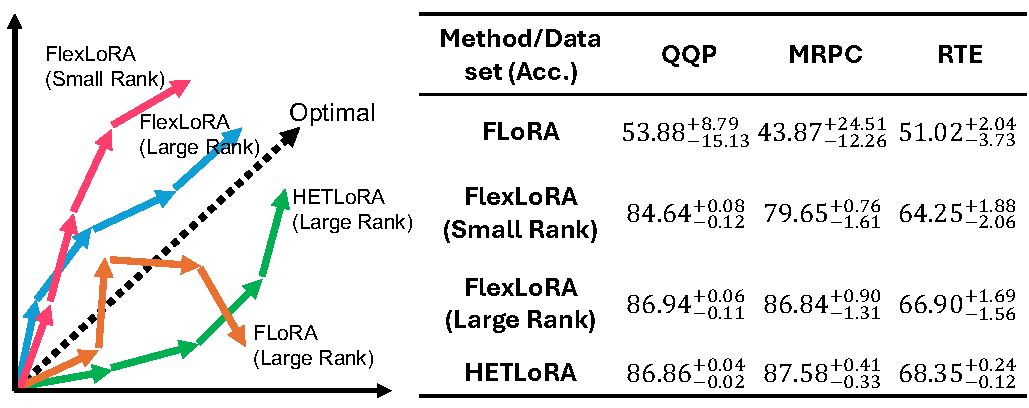
\includegraphics[width=0.80\linewidth]{fig/motivation.pdf}
    \caption{The intuitive convergence trajectories of existing methods and empirical results on three datasets in homogeneous settings.}
    \label{fig:motivation}
    % \vspace{-10pt}
\end{figure}


As discussed in Section~\ref{subsec:baselines}, existing federated LoRA-based fine-tuning methods suffer from different levels of initialization and aggregation noise. To isolate these effects, Figure~\ref{fig:motivation} illustrates optimization trajectories and empirical results. In this setup, we fix the LoRA rank across clients to remove initialization noise for FlexLoRA and HETLoRA, allowing a clearer focus on their aggregation noise (detailed settings in \supplement{Appendix Section~\ref{appendixsubsection:other_settings}}).

The results show that FLoRA, while free of aggregation noise, struggles due to random initialization, yielding low accuracies of 53.88\%, 43.87\%, and 51.02\% on QQP, MRPC, and RTE. FlexLoRA, by contrast, is mainly affected by its rank-dependent SVD-based aggregation noise: at large ranks (e.g., $r_i=16$) it performs well (86.94\% on QQP), but its accuracy drops at smaller ranks (e.g., 84.64\% at $r_i=1$). HETLoRA introduces bias through its averaging rule, yet achieves strong performance, with 87.58\% on MRPC and 68.35\% on RTE, suggesting its noise can be no worse than FlexLoRA’s. Finally, FlexLoRA incurs heavy computation from repeated SVD, whereas HETLoRA uses a lightweight averaging scheme.


\subsubsection{Impact of Hyperparameters}\label{appendixsubsection:num_ratio}

\begin{table}[h]
  \centering
  \caption{The impacts of the number of TC and clients' HR.}
  \renewcommand{\arraystretch}{1.2} 
  \scalebox{0.95}{
  \begin{tabular}{c|ccccc}
    \toprule[1.5pt]
    \multicolumn{1}{c|}{\multirow{3}{*}{\textbf{Method}}} & \multicolumn{3}{c}{\textbf{CoLA Dataset}} \\
    \multicolumn{1}{c|}{} & \shortstack{\textbf{TC=100}\\\textbf{HR=1:1:1}} & \shortstack{\textbf{TC=200}\\\textbf{HR=1:1:1}} & \shortstack{\textbf{TC=100}\\\textbf{HR=6:3:1}} \\
    \midrule
      FLoRA  &  $-4.08$ &$-2.07$ &$-2.07$\\
    FlexLoRA & $13.42$  &$-4.73$ &$-2.50$  \\
    HETLoRA  &  $48.09$ &$50.54$ &$51.04$\\
    \textbf{Fed-PLoRA} & \boldmath{$59.38$} & \boldmath{$55.56$} & \boldmath{$58.28$}  \\
    \bottomrule[1.5pt]
  \end{tabular}
  }
  \label{tab:abl_tc_hr}
\end{table}


\textbf{The Impact of Total Clients and Resource Heterogeneity.} We study how the total number of clients (TC) and the heterogeneity ratio (HR) of client resources affect performance. Table~\ref{tab:abl_tc_hr} reports results on CoLA. Across all configurations, Fed-PLoRA consistently outperforms baselines (FLoRA, FlexLoRA, HETLoRA). Increasing TC from 100 to 200 (with balanced HR=1:1:1) slightly reduces Fed-PLoRA’s score (59.38\% to 55.56\%) but still keeps a clear margin over HETLoRA (50.54\%). When shifting HR from balanced (1:1:1) to skewed (6:3:1, more low-resource clients) with TC=100, Fed-PLoRA remains robust (59.38\% to 58.28\%). These results show that Fed-PLoRA scales well with both client population and resource imbalance. 



\begin{table}[h]
  \centering
  \caption{The impacts of the heterogeneous rank setting.}
  \renewcommand{\arraystretch}{1.2} 
  \scalebox{0.95}{
  \begin{tabular}{c|cccccc}
    \toprule[1.2pt]
    \multicolumn{1}{c|}{\multirow{3}{*}{\textbf{Method}}} & \multicolumn{4}{c}{\textbf{CoLA Dataset}} \\
    \multicolumn{1}{c|}{} & \shortstack{\textbf{Ranks}\\\textbf{1/2/4}} & \shortstack{\textbf{Ranks}\\\textbf{1/2/16}} & \shortstack{\textbf{Ranks}\\\textbf{1/4/16}}& \shortstack{\textbf{Ranks}\\\textbf{2/8/16}} \\
    \midrule
      FLoRA  &  $-2.07$ &$-2.07$ & $-4.08$ &$-2.07$\\
    FlexLoRA & $1.01$  &$4.16$ &$13.42$ &$-3.76$  \\
    HETLoRA  & $47.44$ &$46.70$ &$48.09$ &$49.54$\\
    \textbf{Fed-PLoRA} & \boldmath{$58.58$} & \boldmath{$60.26$} & \boldmath{$59.38$} & \boldmath{$60.41$}  \\
    \bottomrule[1.2pt]
  \end{tabular}
  }
  \label{tab:abl_rank_setting}
\end{table}

\textbf{The Impact of Client Rank Settings.} We evaluate how different distributions of LoRA ranks across clients influence performance, with results on CoLA shown in Table~\ref{tab:abl_rank_setting}. Rank configurations tested include \{1, 2, 4\}, \{1, 2, 16\}, \{1, 4, 16\}, and \{2, 8, 16\}, under the same settings as the main experiments. Fed-PLoRA consistently achieves the highest Matthews Correlation scores, outperforming FLoRA, FlexLoRA, and HETLoRA across all cases. For example, Fed-PLoRA attains 58.58\% with ranks 1/2/4 and 60.41\% with ranks 2/8/16, demonstrating strong robustness and adaptability to heterogeneous client resources. 




\begin{table*}[h]
\centering
\caption{Performance and resource usage of different methods under extremely large global model rank.}
\renewcommand{\arraystretch}{1.2} 
\scalebox{0.55}{
\begin{tabular}{cc|cccc|cccc}
\toprule[1.4pt]
\multicolumn{2}{c|}{\textbf{\shortstack{Method \\ ~}}} & 
\textbf{\shortstack{CoLA \\ Matthews Corr.}} & 
\textbf{\shortstack{SST-2 \\ Accuracy}} & 
\textbf{\shortstack{MRPC \\ Accuracy}} & 
\textbf{\shortstack{RTE \\ Accuracy}} & 
\textbf{\shortstack{Client FLOPs \\ GFLOPS}} & 
\textbf{\shortstack{Server FLOPs \\ MFLOPS}} & 
\textbf{\shortstack{Throughput \\ seconds / 100 tokens}} & 
\textbf{\shortstack{Uplink/Downlink \\ MB / Round}} \\
\midrule
\textbf{Homogeneous} 
  & \textbf{FedIT (Rank=$R$)} & $62.94$ & $91.97$ & $88.72$ & $73.28$ & $695.50$ & $5.89$ & $2.33$  & $430.08$ / $430.08$ \\
\midrule
\multirow{4}{*}{\shortstack{\textbf{Heterogeneous} \\ $R=128$ \\ $\max(r_i) = 16$ \\ Avg Rank =7}} 
  & \textbf{FLoRA}         & $-4.98$ & $70.52$ & $31.51$ & $52.70$ & $202.40$ & $74.94$  & $0.89$ & $23.52$ / $235.20$ \\
  & \textbf{FlexLoRA}      & $1.43$  & $50.91$ & $68.38$ & $53.42$ & $202.37$ & $620.20$ & $0.89$ & $23.52$ / $23.52$ \\
  & \textbf{HETLoRA}       & $47.65$ & $71.62$ & $80.88$ & $59.56$ & $202.37$ & $1.71$   & $0.89$ & $23.52$ / $23.52$ \\
  & \textbf{Fed-PLoRA}     & \boldmath{$55.43$} & \boldmath{$72.82$} & \boldmath{$85.04$} & \boldmath{$70.36$} & $202.37$ & $1.71$   & $0.89$ & $23.52$ / $129.36$ \\
\bottomrule[1.4pt]
\end{tabular}
}
\label{appendixtable:large_global_rank}
\end{table*}

\noindent\textbf{The Impact of Extremely Large Global Rank $R$ on Learning Efficiency.} We evaluate the effect of increasing the global model rank to 128 while capping local ranks at 16 to reflect realistic resource constraints. Experiments are conducted on four GLUE tasks under the IID setting with a batch size of 16. Input sequence length is set to 128 for CoLA and SST-2, and 256 for MRPC and RTE.

Client-side FLOPS (including initialization and LoRA operations) are averaged over all clients and rounds on a per-sample basis. Server-side FLOPS measure aggregation costs. Throughput is reported as the average seconds to process 100 training tokens on clients. Communication volume denotes uplink and downlink per round per client in MB under 32-bit precision.

As shown in Table~\ref{appendixtable:large_global_rank}, Fed-PLoRA consistently outperforms other heterogeneous baselines under this extreme $R$. Client-side FLOPS and throughput remain identical across methods since all use the same model structure and simulated hardware. On the server side, Fed-PLoRA matches HETLoRA’s efficiency by aggregating one-rank modules independently. Uplink costs are equally low across all methods, as only trainable LoRA modules are transmitted. The main trade-off is in downlink cost, which scales with $R$ and equals that of FedIT. However, excessively large $R$ is rarely practical under heterogeneous constraints and may even cause divergence, as observed for FLoRA and FlexLoRA on CoLA. Since LoRA is designed for parameter efficiency, setting $R$ close to the hidden dimension provides little benefit and often harms stability. 

\subsubsection{The Impact of Different Configurations of PLoRA}\label{appendixsubsection:plora_rank}

% \begin{table}[h]
%   \centering
%   \caption{The impact of PLoRA's parallel rank size.}
% \renewcommand{\arraystretch}{1.2} 
%   \scalebox{0.85}{
%   \begin{tabular}{c|ccc}
%     \toprule[1.5pt]
%     \multicolumn{1}{c|}{\multirow{2}{*}{\textbf{Method}}} & \multicolumn{1}{c}{\textbf{CoLA (Matthews Correlations)}} \\
%     \multicolumn{1}{c|}{} & \textbf{Equivalent Rank:2/8/16}  \\
%     \midrule
%     Fed-PLoRA (Two-Rank)  & $59.35$\\
%     \textbf{Fed-PLoRA (One-Rank)}  & \boldmath{$60.41$} \\
%     \bottomrule[1.5pt]
%   \end{tabular}
%   }
%   \label{tab:abl_parallel_rank}
% \end{table}

We evaluate how the rank size of individual PLoRA modules influences performance. Specifically, we compare our default one-rank design (Fed-PLoRA (Parallel One-Rank)) with a two-rank variant (Fed-PLoRA (Parallel Two-Rank)), both configured to yield the same total effective LoRA rank across clients with heterogeneous rank settings (2, 8, 16). The one-rank configuration achieves a slightly higher Matthews Correlation score (60.41\%) than the two-rank configuration (59.35\%). This result supports our design choice.  %: parallel one-rank modules provide greater flexibility while maintaining strong performance.


\subsubsection{The Impacts of Dropout}\label{appendixsubsection:dropout}


\begin{table}[h]
  \centering
  \caption{The impacts of dropout in the PLoRA.}
\renewcommand{\arraystretch}{1.2} 
  \scalebox{0.85}{
  \begin{tabular}{c|cc}
    \toprule[1.5pt]
    \multirow{3}{*}{\textbf{Method}} & \multicolumn{2}{c}{\textbf{Dolly-15K (Rouge-L)}} \\
    & \multicolumn{2}{c}{\textbf{Rank: 1/8/32}} \\
    & \textbf{IID} & \textbf{non-IID} \\
    \midrule
    Fed-PLoRA (Unfold, w/ Dropout) & 60.07 & 59.70 \\
    \textbf{Fed-PLoRA}              & 60.07 & 59.69 \\
    \bottomrule[1.5pt]
  \end{tabular}
  }
  \label{tab:dropout}
\end{table}

We investigate the impact of applying LoRA dropout within the Fed-PLoRA framework. Typically, dropout layers are utilized for regularization before input features pass into LoRA modules (specifically, before the LoRA $\mathbf{A}$ matrix). In our Fed-PLoRA approach, the \textit{Select-N-Fold} strategy involves merging non-selected parallel LoRA modules into the main target module. When these modules are folded, any dropout layers specifically associated with these folded LoRA paths are effectively bypassed for those components in subsequent forward passes. This characteristic motivates an evaluation to understand how performance is affected by dropout under our folding mechanism.
%
Table~\ref{tab:dropout} presents a comparison on the Dolly-15K dataset (Rouge-L score), with client ranks set to (1, 8, 32). We compare a variant termed ``Fed-PLoRA (Unfold, w/ Dropout)'', where we assume modules are frozen but kept unfolded, allowing standard LoRA dropout to be active on all PLoRA modules against our standard Fed-PLoRA configuration, but with higher computational costs. The results show minimal differences between the two approaches across both IID and non-IID data distributions. In the IID setting, both configurations achieve a Rouge-L score of 60.07\%. In the non-IID setting, ``Fed-PLoRA (Unfold, w/ Dropout)'' achieves 59.70\%, while our method achieves 59.69\%. These nearly identical results suggest that not using dropout on frozen layers does not affect the performance.

\subsubsection{More Visualization on Cosine Similarities across PLoRA Modules.}\label{appendixsubsection:vis_cos_sim}


\begin{figure*}[h]
    \centering
    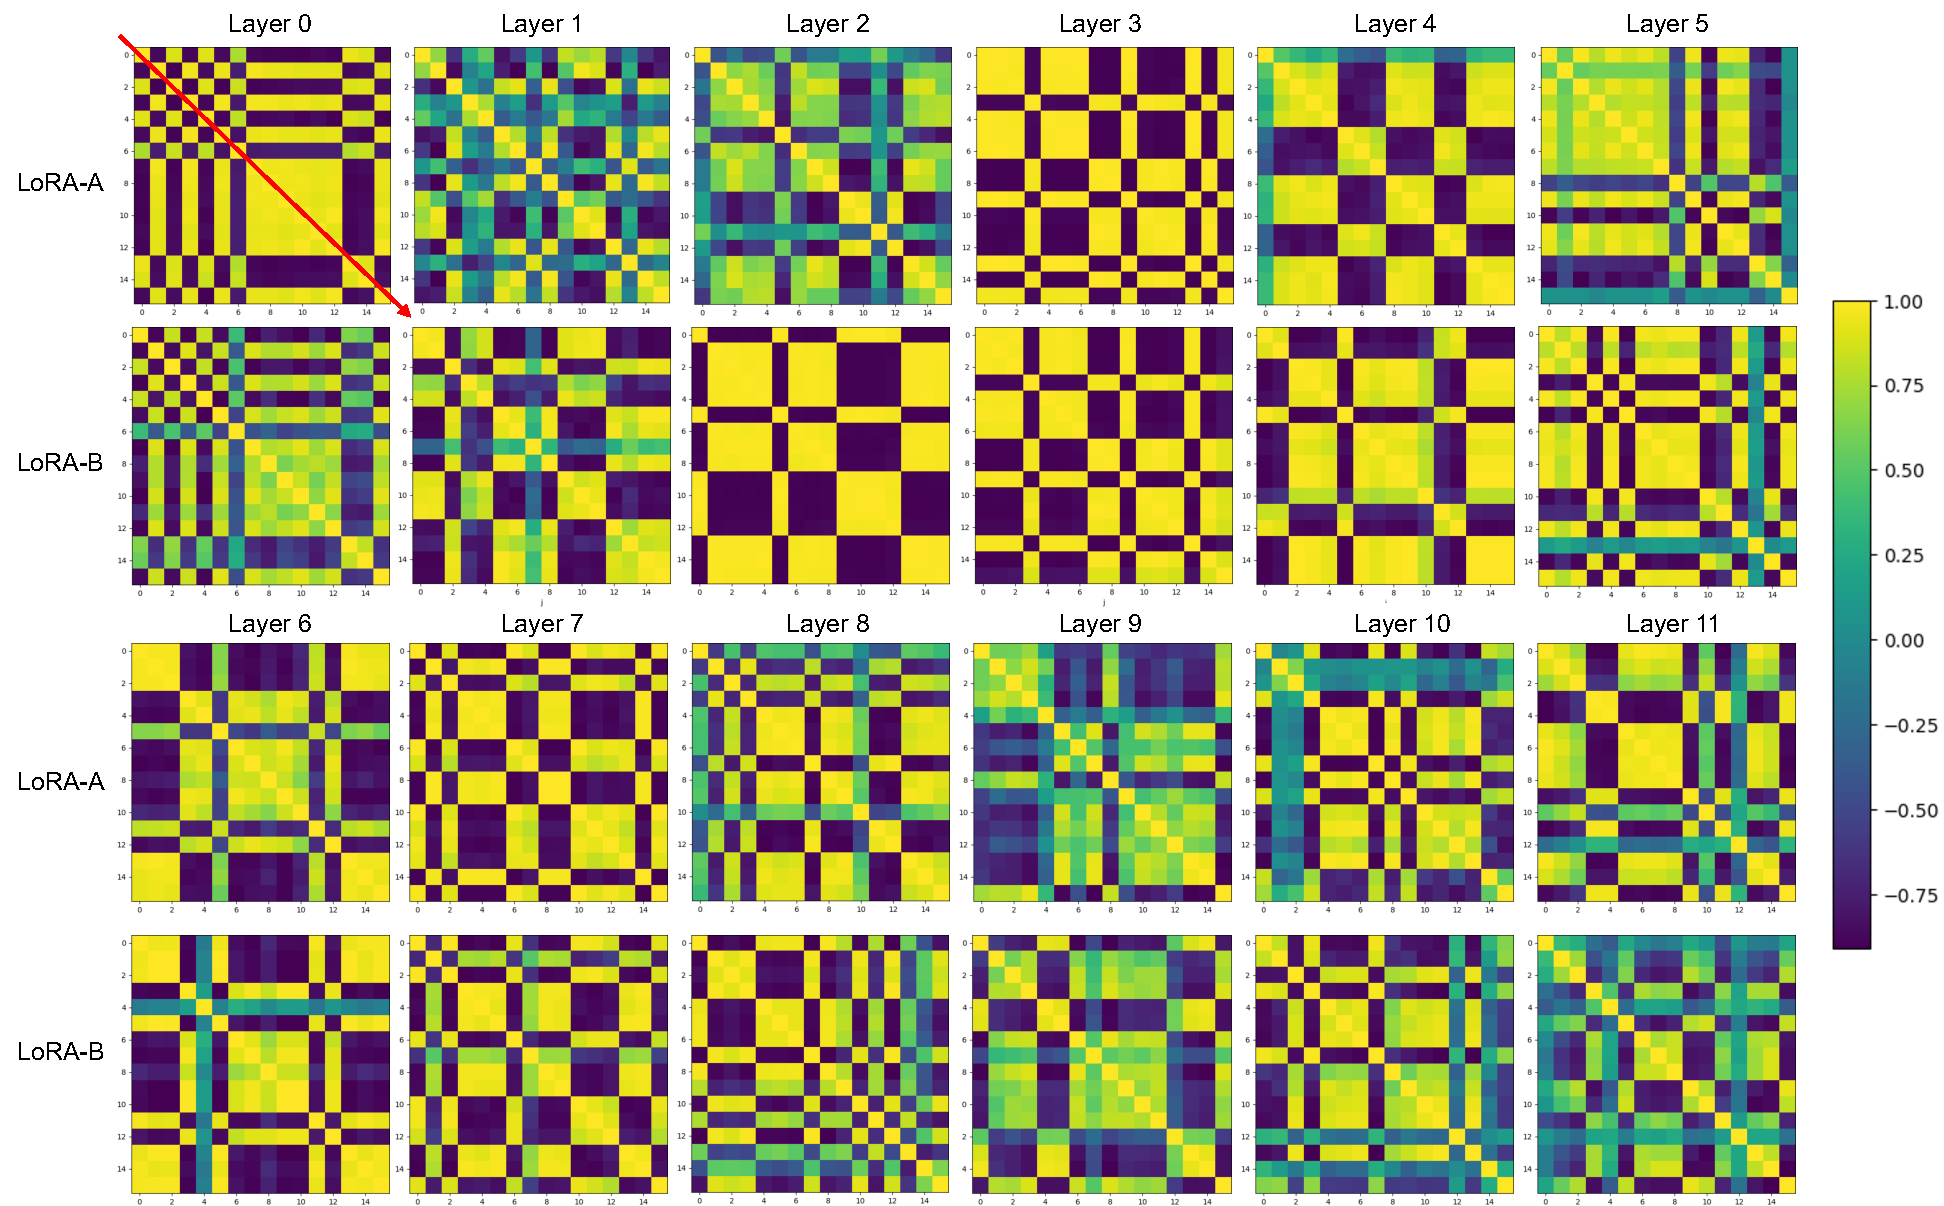
\includegraphics[width=0.98\linewidth]{fig/sim-appendix.pdf}
    \caption{Cosine similarity heatmaps of PLoRA modules on the non-IID RTE dataset (averaged over all rounds). Each block reports pairwise similarities of modules across clients for LoRA-A and LoRA-B, spanning layers 0 through 11.}
    \label{fig:vis_sim_appendix}
    % \vspace{-10pt}
\end{figure*}

To analyze the aggregation noise in Fed-PLoRA, we visualize the cosine similarity heatmaps across clients' PLoRA modules for the Query weights in all 12 transformer layers of BERT-base, averaged over all rounds. Both $A$ and $B$ module similarities are shown. According to Section~\ref{appendixsec:analysis}, when $\mathbf{A}_{i,(j)}^t \approx \overline{\mathbf{A}}_{(j)}^t$ or $\mathbf{B}_{i,(j)}^t \approx \overline{\mathbf{B}}_{(j)}^t$, aggregation noise of Fed-PLoRA is minimized. Figure~\ref{fig:vis_sim_appendix} reveals consistently high similarity values (near 1.0) along diagonal and cross-wise patterns, particularly highlighted by the red arrow in Layer 0's LoRA-A, suggesting strong similarity among certain ranks. Moreover, we observe that some consecutive layers maintain high inter-client similarity, indicating that even under non-IID settings, certain ranks learn overlapping or redundant features, potentially pointing to shared semantic structures across clients. 

This pattern emerges naturally from the design of Fed-PLoRA. Since each client receives the full set of $R$ global PLoRA modules and selects a subset for local training, all modules remain aligned in initialization across rounds. The random selection mechanism ensures that over time, every rank-$j$ module is trained by a diverse subset of clients, leading to gradual synchronization of parameters across the population. Furthermore, the frozen folded modules help preserve the global structure even on clients with limited capacity, reducing noise accumulation across rounds. As a result, frequently selected ranks tend to exhibit strong inter-client alignment, while occasionally selected modules still retain structural consistency due to their shared initialization and partial update history. This design promotes implicit coordination among clients and contributes to the observed high cosine similarity, thereby reducing the aggregation noise without explicit regularization or coordination.

While our method does not entirely eliminate aggregation noise. This is a characteristic shared with several other federated LoRA-based fine-tuning methods, such as FedIT and HETLoRA. However, we note that there is a growing body of research in the literature~\cite{sun2024improving,guo2024selective} focused on improving the aggregation of LoRA in the homogeneous setting. We will explore the integration of these methods with Fed-PLoRA in heterogeneous settings in our future research.


\section{Detailed Analysis of Initialization and Aggregation Noise}\label{appendixsec:analysis}


This section investigates the noise arising from initialization and aggregation processes in heterogeneous federated LoRA-based fine-tuning methods. 


% \subsection{Optimal initialization and aggregation}
% \label{appsec:optimal_aggregation}

% To solve the problem in Equation~\eqref{}
% Let $\mathbf{A}$ and $\mathbf{B}$ denote the global LoRA matrices distributed by the server at the beginning of a communication round. Each client $i \in [v]$ then performs local fine-tuning, computing updates $\Delta\mathbf{A}_i$ and $\Delta\mathbf{B}_i$ to these matrices based on its local dataset. The client's LoRA matrices post-local training are thus $(\mathbf{A}+\Delta\mathbf{A}_i)$ and $(\mathbf{B}+\Delta\mathbf{B}_i)$.

% % We first represent the optimal LoRA aggregation.

% The optimal aggregated base layer update, denoted as $\Delta \boldsymbol{\mathcal{W}}^*$, is defined as the average of these client-specific LoRA matrix products:
% \begin{align}
% \Delta \boldsymbol{\mathcal{W}}^* &= \frac{1}{v}\sum_{i\in[v]} (\mathbf{B}+\Delta\mathbf{B}_i) (\mathbf{A}+\Delta\mathbf{A}_i) \\
% &= \frac{1}{v} \sum_{i\in[v]} \left( \mathbf{B}\mathbf{A} + \mathbf{B}\Delta\mathbf{A}_i + \Delta\mathbf{B}_i\mathbf{A} + \Delta\mathbf{B}_i\Delta\mathbf{A}_i \right) \notag \\
% &= \mathbf{B}\mathbf{A} + \frac{1}{v} \sum_{i\in[v]} \left( \mathbf{B} \Delta \mathbf{A}_i + \Delta \mathbf{B}_i \mathbf{A} \right) + \frac{1}{v} \sum_{i\in[v]} \Delta \mathbf{B}_i \Delta \mathbf{A}_i
% \end{align}
% Here, $\mathbf{B}\mathbf{A}$ represents the initial global LoRA product, while the subsequent terms capture the averaged linear and quadratic update contributions.

% Following server-side aggregation, new LoRA parameters derived from $\Delta \boldsymbol{\mathcal{W}}^*$ are distributed to clients for the next round of training. This initialization can introduce a discrepancy in the client's local optimization. We term this ``initialization noise'' and quantify it by measuring the change in local gradients.
% Assume the model's prediction $\hat{y}$ for an input $x$ is given by a frozen base layer $\boldsymbol{\mathcal{W}}_{\text{base}}$ and a trainable LoRA component:
% \[
% \hat{y} = \boldsymbol{\mathcal{W}}_{\text{base}}x + \mathbf{B} \mathbf{A} x
% \]
% Let the loss function be $\mathcal{L}(\hat{y}, y)$. The gradient of the loss with respect to the LoRA component's output $\mathbf{B} \mathbf{A} x$ is $\nabla_{\hat{y}} \mathcal{L} = \frac{\partial \mathcal{L}}{\partial \hat{y}} \in \mathbb{R}^{d}$.

% The gradients of the loss with respect to the LoRA matrices $\mathbf{B}^t$ and $\mathbf{A}^t$ at the end of local training in round $t$ are:
% \[
% \nabla_{\mathbf{B}^{t}} \mathcal{L}^{t} = \nabla_{\hat{y}} \mathcal{L}^{t} \cdot (\mathbf{A}^{t} x)^\top
% \]
% \[
% \nabla_{\mathbf{A}^{t}} \mathcal{L}^{t} = (\mathbf{B}^{t})^\top \nabla_{\hat{y}} \mathcal{L}^{t} \cdot x^\top
% \]
% For the subsequent round $t+1$, clients initialize their LoRA components with matrices ${\mathbf{A}^*}^{t+1}$ and ${\mathbf{B}^*}^{t+1}$, which are ideally derived such that ${\mathbf{B}^*}^{t+1}{\mathbf{A}^*}^{t+1} = \Delta \boldsymbol{\mathcal{W}}^*$. The gradients at the start of round $t+1$ are:
% \[
% \nabla_{{\mathbf{B}^*}^{t+1}} \mathcal{L}^{t+1} = \nabla_{\hat{y}} \mathcal{L}^{t+1} \cdot ({\mathbf{A}^*}^{t+1} x)^\top
% \]
% \[
% \nabla_{{\mathbf{A}^*}^{t+1}} \mathcal{L}^{t+1} = ({\mathbf{B}^*}^{t+1})^\top \nabla_{\hat{y}} \mathcal{L}^{t+1} \cdot x^\top
% \]
% The initialization noise is then measured by the L2-norm of the difference between these consecutive gradients:
% \[
% \delta_{\mathbf{B}^*} = \left\| \nabla_{{\mathbf{B}^*}^{t+1}} \mathcal{L}^{t+1} - \nabla_{\mathbf{B}^{t}} \mathcal{L}^{t} \right\|_2
% \]
% \[
% \delta_{\mathbf{A}^*} = \left\| \nabla_{{\mathbf{A}^*}^{t+1}} \mathcal{L}^{t+1} - \nabla_{\mathbf{A}^{t}} \mathcal{L}^{t} \right\|_2
% \]
% Significant values of $\delta_{\mathbf{A}^*}$ or $\delta_{\mathbf{B}^*}$ indicate a substantial perturbation to the client's optimization process. This occurs because even if the aggregated product $\Delta \boldsymbol{\mathcal{W}}^*$ is optimal, its specific initializations for ${\mathbf{A}^*}^{t+1}$ and ${\mathbf{B}^*}^{t+1}$ may not align with the client's parameter state ($\mathbf{A}^{t}, \mathbf{B}^{t}$) at the end of its local training, thereby redirecting the subsequent local optimization path.

We use the following general definitions for noise as established in the main paper:
Let $\boldsymbol{\theta}^{t-1} = (\mat{A}^{t-1}, \mat{B}^{t-1})$ be the global LoRA parameters from the server at the end of round $t-1$ (with global rank $R$).
Let $\boldsymbol{\theta}_i^{t-1} = (\mat{A}_i^{t-1}, \mat{B}_i^{t-1})$ be the local LoRA parameters with which client $i$ (from a set of $v$ clients) starts round $t$ (with local rank $r_i$).
The \textbf{Initialization Noise} at the beginning of round $t$ is:
$$\mathcal{N}_{\text{Init}}^{t} := \sum_{i=1}^{v} \left(\left\|{\mat{A}}^{t-1}\ominus {\mat{A}}_i^{t-1}\right\|_F + \left\|{\mat{B}}^{t-1}\ominus {\mat{B}}_i^{t-1}\right\|_F\right)$$
Here, $\mat{X} \ominus \mat{Y}$ signifies the part of $\mat{X}$ not captured by $\mat{Y}$.

After local training, client $i$ produces updated LoRA parameters $\boldsymbol{\theta}_i^t = (\mat{A}_i^t, \mat{B}_i^t)$.
The ideal aggregated target module update is $\Delta \boldsymbol{\mathcal{W}}_{*}^t = \frac{1}{v}\sum_{i=1}^{v} \mat{B}_i^t \mat{A}_i^t$.
The actual aggregated target module update by a specific method is $\Delta\boldsymbol{\mathcal{W}}^t=\mat{B}^t \mat{A}^t$, where $\mat{A}^t, \mat{B}^t$ are the global LoRA parameters after aggregation at round $t$.
The \textbf{Aggregation Noise} at the end of round $t$ is:
$$\mathcal{N}_{\text{Agg}}^{t} := \left\| \Delta \boldsymbol{\mathcal{W}}_{*}^t - \Delta \boldsymbol{\mathcal{W}}^t \right\|_F$$


\subsection{FLoRA} \label{appendixsubsection:flora}
FLoRA~\cite{wangflora} employs a stacking-based aggregation. For initialization, client LoRA modules $\mat{A}_i^{t-1}$ are randomly initialized (e.g., Gaussian Distribution), and $\mat{B}_i^{t-1}$ is initialized to zeros at each round $t$.

\textbf{Initialization Noise ($\mathcal{N}_{\text{FLoRA\_Init}}^{t}$):} Given $\mat{A}_i^{t-1}$ is random and $\mat{B}_i^{t-1} = \mat{0}$, these local parameters do not retain information from the previous global LoRA parameters $\mat{A}^{t-1}$ and $\mat{B}^{t-1}$. For $\mat{B}$ matrices: Since $\mat{B}_i^{t-1} = \mat{0}$, the part of $\mat{B}^{t-1}$ not captured by $\mat{B}_i^{t-1}$ is $\mat{B}^{t-1}$ itself. Thus, $\left\|{\mat{B}}^{t-1}\ominus {\mat{B}}_i^{t-1}\right\|_F = \left\|{\mat{B}}^{t-1}\right\|_F$. For $\mat{A}$ matrices: $\mat{A}_i^{t-1}$ is random and independent of $\mat{A}^{t-1}$. It does not systematically capture any part of $\mat{A}^{t-1}$. The initialization noise is formulated as:
\begin{align*}
\mathcal{N}_{\text{FLoRA\_Init}}^{t} &= \sum_{i=1}^{v} \left(\left\|{\mat{A}}^{t-1}\ominus {\mat{A}}_i^{t-1}\right\|_F + \left\|{\mat{B}}^{t-1}\ominus {\mat{B}}_i^{t-1}\right\|_F\right) \\
&\approx \sum_{i=1}^{v} \left( \left\|{\mat{A}}^{t-1}\right\|_F + \left\|{\mat{B}}^{t-1}\right\|_F \right) + \sigma^2
\end{align*}
where $\sigma^2$ denotes the magnitude of the random noise used for initializing $\mathbf{A}$ matrix. This noise is substantial.

\textbf{Aggregation Noise ($\mathcal{N}_{\text{FLoRA\_Agg}}^{t}$):} FLoRA stacks client LoRA modules. Let client $i$ have $\mat{A}_i^t \in \mathbb{R}^{r_i \times k}$ and $\mat{B}_i^t \in \mathbb{R}^{d \times r_i}$.
The server forms:
$$\mat{A}_{}^t = \begin{pmatrix} \mat{A}_1^t \\ \vdots \\ \mat{A}_v^t \end{pmatrix} \in \mathbb{R}^{(\sum r_i) \times k} \quad \text{and} \quad \mat{B}_{}^t = \begin{pmatrix} \mat{B}_1^t & \cdots & \mat{B}_v^t \end{pmatrix} \in \mathbb{R}^{d \times (\sum r_i)}$$
The aggregated update is $\Delta\boldsymbol{\mathcal{W}}_{\text{FLoRA}}^t = \frac{1}{v} \mat{B}_{}^t \mat{A}_{}^t$.
The product is $\mat{B}_{}^t \mat{A}_{}^t = \sum_{i\in[v]} \mat{B}_i^t \mat{A}_i^t$.
So, the actual aggregated update is:
$$\Delta\boldsymbol{\mathcal{W}}_{\text{FLoRA}}^t = \frac{1}{v} \sum_{i\in[v]} \mat{B}_i^t \mat{A}_i^t$$
The ideal target module update is $\Delta \boldsymbol{\mathcal{W}}_{*}^t = \frac{1}{v} \sum_{i\in[v]} \mat{B}_i^t \mat{A}_i^t$.
Therefore, the aggregation noise is:
\begin{align*}
\mathcal{N}_{\text{FLoRA\_Agg}}^{t} &= \left\| \Delta \boldsymbol{\mathcal{W}}_{*}^t - \Delta \boldsymbol{\mathcal{W}}_{\text{FLoRA}}^t \right\|_F \\
&= \left\| \frac{1}{v} \sum_{i\in[v]} \mat{B}_i^t \mat{A}_i^t - \frac{1}{v} \sum_{i\in[v]} \mat{B}_i^t \mat{A}_i^t \right\|_F = 0
\end{align*}

\subsection{FlexLoRA} \label{appendixsubsection:flexlora}
FlexLoRA aggregates LoRA modules in full weight space, then uses SVD for local LoRA modules. Clients truncate these for initialization.

\textbf{Initialization Noise ($\mathcal{N}_{\text{FlexLoRA\_Init}}^{t}$):} The server has global LoRA modules $\mat{A}^{t-1}$ (from SVD, rank $R$) and $\mat{B}^{t-1}$ (from SVD, rank $R$).
Client $i$ (rank $r_i \le R$) initializes by truncation:
$\mat{A}_i^{t-1} = \mat{A}^{t-1}_{[:r_i, :]}$ (first $r_i$ rows of $\mat{A}^{t-1}$).
$\mat{B}_i^{t-1} = \mat{B}^{t-1}_{[:, :r_i]}$ (first $r_i$ columns of $\mat{B}^{t-1}$).
The part of $\mat{A}^{t-1}$ not captured is $\mat{A}^{t-1}_{[r_i+1:R, :]}$.
The part of $\mat{B}^{t-1}$ not captured is $\mat{B}^{t-1}_{[:, r_i+1:R]}$. The initialization noise is then formulated as,
\begin{align*}
\mathcal{N}_{\text{FlexLoRA\_Init}}^{t} &= \sum_{i\in[v]} \left(\left\|{\mat{A}}^{t-1}\ominus {\mat{A}}_i^{t-1}\right\|_F + \left\|{\mat{B}}^{t-1}\ominus {\mat{B}}_i^{t-1}\right\|_F\right) \\
&= \sum_{i\in[v]} \left( \left\| \mat{A}^{t-1}_{[r_i+1:R, :]} \right\|_F + \left\| \mat{B}^{t-1}_{[:, r_i+1:R]} \right\|_F \right)
\end{align*}
This noise is non-zero if any $r_i < R$.

\textbf{Aggregation Noise ($\mathcal{N}_{\text{FlexLoRA\_Agg}}^{t}$):} Clients send $\mat{A}_i^t, \mat{B}_i^t$. The server computes the ideal average update:
$$\Delta \boldsymbol{\mathcal{W}}_{*}^t = \frac{1}{v}\sum_{i=1}^{v}\mat{B}_i^t \mat{A}_i^t$$
However, FlexLoRA then performs SVD on $\Delta \boldsymbol{\mathcal{W}}_{*}^t$ to get a rank-$R$ approximation:
$$\Delta\boldsymbol{\mathcal{W}}_{\text{FlexLoRA}}^t = \text{SVD}(\Delta \boldsymbol{\mathcal{W}}_{*}^t) = \mat{U}^t \mat{S}^t (\mat{V}^t)^\top$$
The aggregation noise is the SVD truncation error:
\begin{align*}
\mathcal{N}_{\text{FlexLoRA\_Agg}}^{t} &= \left\| \Delta \boldsymbol{\mathcal{W}}_{*}^t - \Delta\boldsymbol{\mathcal{W}}_{\text{FlexLoRA}}^t \right\|_F \\
&= \left\| \Delta \boldsymbol{\mathcal{W}}_{*}^t - \mat{U}^t \mat{S}^t (\mat{V}^t)^\top \right\|_F
\end{align*}


\subsection{HETLoRA}
\label{appendixsubsection:hetlora}

% The HETLoRA aggregation strategy diverges from the optimal approach outlined in Section~\ref{appsec:optimal_aggregation}. Instead of averaging the complete LoRA update products $(\mathbf{B}+\Delta\mathbf{B}_i)(\mathbf{A}+\Delta\mathbf{A}_i)$ from each client, HETLoRA computes the average of the LoRA update $\Delta\mathbf{A}_i$ and $\Delta\mathbf{B}_i$ separately across all clients. These averaged updates are then added to the initial global LoRA matrices $\mathbf{A}$ and $\mathbf{B}$, and the product of these resulting matrices forms the aggregated update, $\Delta \boldsymbol{\mathcal{W}}_{\text{HETLoRA}}$.

% Let $\bar{\Delta\mathbf{A}} = \frac{1}{v} \sum_{i\in[v]} \Delta \mathbf{A}_i$ and $\bar{\Delta\mathbf{B}} = \frac{1}{v} \sum_{i\in[v]} \Delta \mathbf{B}_i$. The aggregated update is then:
% \begin{align}
% \Delta \boldsymbol{\mathcal{W}}_{\text{HETLoRA}} &= \left(\mathbf{B} + \bar{\Delta\mathbf{B}}\right) \left(\mathbf{A} + \bar{\Delta\mathbf{A}}\right) \\
% &= \left(\mathbf{B} + \frac{1}{v} \sum_{k\in[v]} \Delta \mathbf{B}_k\right) \left(\mathbf{A} + \frac{1}{v} \sum_{l\in[v]} \Delta \mathbf{A}_l\right)
% \end{align}
% For a system with $v=5$ clients, this expands to:
% \begin{align}
% \Delta \boldsymbol{\mathcal{W}}_{\text{HETLoRA}}
% &= \left(\mathbf{B} + \frac{1}{5} \sum_{k=0}^{4} \Delta \mathbf{B}_k\right) \left(\mathbf{A} + \frac{1}{5} \sum_{l=0}^{4} \Delta \mathbf{A}_l\right) \notag \\
% &= \mathbf{B}\mathbf{A} + \mathbf{B}\left(\frac{1}{5}\sum_{l=0}^{4} \Delta\mathbf{A}_l\right) + \left(\frac{1}{5}\sum_{k=0}^{4} \Delta\mathbf{B}_k\right)\mathbf{A} + \left(\frac{1}{5}\sum_{k=0}^{4} \Delta\mathbf{B}_k\right)\left(\frac{1}{5}\sum_{l=0}^{4} \Delta\mathbf{A}_l\right) \notag \\
% &= \mathbf{B}\mathbf{A} + \frac{1}{5} \sum_{k=0}^{4} (\mathbf{B}\Delta\mathbf{A}_k + \Delta\mathbf{B}_k\mathbf{A}) + \frac{1}{25} \sum_{k=0}^{4}\sum_{l=0}^{4} \Delta\mathbf{B}_k\Delta\mathbf{A}_l
% \label{eq:hetlora_dw_expansion}
% \end{align}
% Comparing Eq.~\eqref{eq:hetlora_dw_expansion} to the optimal $\Delta \boldsymbol{\mathcal{W}}^*$ (Section~\ref{appsec:optimal_aggregation}), the final term $\frac{1}{25} \sum_{k=0}^{4}\sum_{l=0}^{4} \Delta\mathbf{B}_k\Delta\mathbf{A}_l$ includes cross-client interaction terms (i.e., $\Delta\mathbf{B}_k\Delta\mathbf{A}_l$ where $k \neq l$). This differs from the corresponding term $\frac{1}{5}\sum_{k=0}^{4} \Delta\mathbf{B}_k\Delta\mathbf{A}_k$ in $\Delta\boldsymbol{\mathcal{W}}^*$, leading to an aggregation gap.

% The explicit gap between the optimal $\Delta \boldsymbol{\mathcal{W}}^*$ and $\Delta \boldsymbol{\mathcal{W}}_{\text{HETLoRA}}$ is:
% \begin{align}
% \text{Gap}_{\text{HETLoRA}} &= \Delta \boldsymbol{\mathcal{W}}^* - \Delta \boldsymbol{\mathcal{W}}_{\text{HETLoRA}} \notag \\
% &= \left( \frac{1}{5} \sum_{k=0}^{4} \Delta \mathbf{B}_k \Delta \mathbf{A}_k \right) - \left( \frac{1}{25} \sum_{k=0}^{4} \sum_{l=0}^{4} \Delta \mathbf{B}_k \Delta \mathbf{A}_l \right) \notag \\
% % Retaining the user's detailed expansion of the gap for completeness
% &= \frac{1}{5} \left( \Delta \mathbf{B}_0 \Delta \mathbf{A}_0 + \dots + \Delta \mathbf{B}_4 \Delta \mathbf{A}_4 \right) \notag \\
% &\quad - \frac{1}{25} \Big( \Delta \mathbf{B}_0 (\Delta \mathbf{A}_0 + \dots + \Delta \mathbf{A}_4) + \dots + \Delta \mathbf{B}_4 (\Delta \mathbf{A}_0 + \dots + \Delta \mathbf{A}_4) \Big) \notag \\
% &= \frac{1}{25} \Big( (4\Delta \mathbf{B}_0 \Delta \mathbf{A}_0 - \sum_{l \neq 0} \Delta \mathbf{B}_0 \Delta \mathbf{A}_l) + \dots + (4\Delta \mathbf{B}_4 \Delta \mathbf{A}_4 - \sum_{l \neq 4} \Delta \mathbf{B}_4 \Delta \mathbf{A}_l) \Big) \notag \\
% % The user's subsequent factored forms are also correct representations.
% % Example of one factored form:
% &= \frac{1}{25} \sum_{k=0}^{4} \left( \Delta \mathbf{B}_k (4\Delta \mathbf{A}_k - \sum_{l \neq k} \Delta \mathbf{A}_l) \right)
% \end{align}
% This discrepancy, termed "aggregation noise," arises from the heterogeneous nature of client updates. The gap vanishes if client updates are homogeneous (i.e., $\Delta\mathbf{A}_k = {\Delta\mathbf{A}}$ for all $k$, or $\Delta\mathbf{B}_k = {\Delta\mathbf{B}}$ for all $k$).

% For the subsequent round $t+1$, the LoRA matrices $\mathbf{A}^{\text{init}}$ and $\mathbf{B}^{\text{init}}$ used by clients are precisely these server-aggregated updates applied to the global LoRA matrices from the start of the round:
% \begin{align}
%     \mathbf{A}^{\text{init}} = \mathbf{A} + \frac{1}{v} \sum_{i\in[v]} \Delta \mathbf{A}_i \quad \text{and} \quad \mathbf{B}^{\text{init}} = \mathbf{B} + \frac{1}{v} \sum_{i\in[v]} \Delta \mathbf{B}_i
% \end{align}
% The client model output in round $t+1$ is $\hat{y}^{t+1} = \boldsymbol{\mathcal{W}}_{\text{base}}^{t+1}x + \mathbf{B}^{\text{init}} \mathbf{A}^{\text{init}} x$. The gradients at the end of round $t$ ($\nabla_{\mathbf{B}^{t}} \mathcal{L}^{t}, \nabla_{\mathbf{A}^{t}} \mathcal{L}^{t}$) are compared with those at the start of round $t+1$ using HETLoRA's $\mathbf{A}^{\text{init}}, \mathbf{B}^{\text{init}}$ parameters ($\nabla_{\mathbf{B}^{\text{init}}} \mathcal{L}^{t+1}, \nabla_{\mathbf{A}^{\text{init}}} \mathcal{L}^{t+1}$). The initialization noise is measured as:
% \begin{align}
% \delta_{\mathbf{B}}^{\text{init}} = \left\| \nabla_{\mathbf{B}^{\text{init}}} \mathcal{L}^{t+1} - \nabla_{\mathbf{B}^{t}} \mathcal{L}^{t} \right\|_2
% \end{align}
% \begin{align}
% \delta_{\mathbf{A}}^{\text{init}} = \left\| \nabla_{\mathbf{A}^{\text{init}}} \mathcal{L}^{t+1} - \nabla_{\mathbf{A}^{t}} \mathcal{L}^{t} \right\|_2
% \end{align}
% The non-zero aggregation gap ($\text{Gap}_{\text{HETLoRA}}$) implies that $\Delta \boldsymbol{\mathcal{W}}_{\text{HETLoRA}}$ deviates from the optimal $\Delta \boldsymbol{\mathcal{W}}^*$. Consequently, the LoRA component $\mathbf{z}^{t+1} = \mathbf{B}^{\text{init}}\mathbf{A}^{\text{init}}x$ and the resulting prediction $\hat{y}^{t+1}$ differ from what would be achieved with an optimally aggregated update. This can lead to a suboptimal loss value and a perturbed loss gradient $\nabla_{\hat{y}}\mathcal{L}^{t+1}$ at the outset of client training.

% Furthermore, the averaged matrices $\mathbf{A}^{\text{init}}$ and $\mathbf{B}^{\text{init}}$, while reflecting a consensus, may not align with any specific client's LoRA parameters ($\mathbf{A}^t, \mathbf{B}^t$) from the end of its local training in round $t$. This misalignment is an additional source of noise.

% These combined effects can impair convergence efficiency and stability during the local fine-tuning stages within the HETLoRA framework. 

% Therefore, the initialization noise terms $\delta_{\mathbf{A}}^{\text{init}}$ and $\delta_{\mathbf{B}}^{\text{init}}$ in HETLoRA can be substantial due to a compound effect
% \begin{enumerate}
%     \item \textit{Deviation from Optimal Aggregation Path:} The inherent aggregation gap means the global model update is itself suboptimal, potentially misguiding the collective learning trajectory from the ideal path defined by $\Delta\boldsymbol{\mathcal{W}}^*$.
%     \item \textit{Client-Level Gradient Inconsistency:} The re-initialization of client LoRA parameters with the averaged factors ($\mathbf{A}^{\text{init}}, \mathbf{B}^{\text{init}}$) introduces a discontinuity from the client's prior optimization state, leading to shifts in local gradient computations.
% \end{enumerate}

% \begin{align}
% \Delta \boldsymbol{\mathcal{W}} 
% &= \left(\mathbf{B} + \frac{1}{5} \sum_{i=0}^{4} \Delta \mathbf{B}_i\right)
%    \left(\mathbf{A} + \frac{1}{5} \sum_{i=0}^{4} \Delta \mathbf{A}_i\right) \\
% &= \mathbf{B} \mathbf{A} 
% + \frac{1}{5} \left( \mathbf{B} \Delta \mathbf{A}_0 + \mathbf{B} \Delta \mathbf{A}_1 + \mathbf{B} \Delta \mathbf{A}_2 + \mathbf{B} \Delta \mathbf{A}_3 + \mathbf{B} \Delta \mathbf{A}_4 \right) \notag \\
% &\quad + \frac{1}{5} \left( \Delta \mathbf{B}_0 \mathbf{A} + \Delta \mathbf{B}_1 \mathbf{A} + \Delta \mathbf{B}_2 \mathbf{A} + \Delta \mathbf{B}_3 \mathbf{A} + \Delta \mathbf{B}_4 \mathbf{A} \right) \notag \\
% &\quad + \frac{1}{25} \Big(
% \Delta \mathbf{B}_0 \Delta \mathbf{A}_0 + \Delta \mathbf{B}_0 \Delta \mathbf{A}_1 + \Delta \mathbf{B}_0 \Delta \mathbf{A}_2 + \Delta \mathbf{B}_0 \Delta \mathbf{A}_3 + \Delta \mathbf{B}_0 \Delta \mathbf{A}_4 \notag \\
% &\qquad + \Delta \mathbf{B}_1 \Delta \mathbf{A}_0 + \Delta \mathbf{B}_1 \Delta \mathbf{A}_1 + \Delta \mathbf{B}_1 \Delta \mathbf{A}_2 + \Delta \mathbf{B}_1 \Delta \mathbf{A}_3 + \Delta \mathbf{B}_1 \Delta \mathbf{A}_4 \notag \\
% &\qquad + \Delta \mathbf{B}_2 \Delta \mathbf{A}_0 + \Delta \mathbf{B}_2 \Delta \mathbf{A}_1 + \Delta \mathbf{B}_2 \Delta \mathbf{A}_2 + \Delta \mathbf{B}_2 \Delta \mathbf{A}_3 + \Delta \mathbf{B}_2 \Delta \mathbf{A}_4 \notag \\
% &\qquad + \Delta \mathbf{B}_3 \Delta \mathbf{A}_0 + \Delta \mathbf{B}_3 \Delta \mathbf{A}_1 + \Delta \mathbf{B}_3 \Delta \mathbf{A}_2 + \Delta \mathbf{B}_3 \Delta \mathbf{A}_3 + \Delta \mathbf{B}_3 \Delta \mathbf{A}_4 \notag \\
% &\qquad + \Delta \mathbf{B}_4 \Delta \mathbf{A}_0 + \Delta \mathbf{B}_4 \Delta \mathbf{A}_1 + \Delta \mathbf{B}_4 \Delta \mathbf{A}_2 + \Delta \mathbf{B}_4 \Delta \mathbf{A}_3 + \Delta \mathbf{B}_4 \Delta \mathbf{A}_4
% \Big) \notag \\
% &= \mathbf{B} \mathbf{A} 
% + \frac{1}{5} \sum_{i=0}^{4}  \left( \mathbf{B} \Delta \mathbf{A}_i 
% + \Delta \mathbf{B}_i \mathbf{A} \right)
% + \frac{1}{25} \sum_{i=0}^{4} \sum_{i=0}^{4} \Delta \mathbf{B}_i \Delta \mathbf{A}_i \notag
% \end{align}

% \begin{align}
% \Delta \boldsymbol{\mathcal{W}}^* - \Delta \boldsymbol{\mathcal{W}}
% &= \left( \frac{1}{5} \sum_{i=0}^{4} \Delta \mathbf{B}_i \Delta \mathbf{A}_i \right)
% - \left( \frac{1}{25} \sum_{i=0}^{4} \sum_{j=0}^{4} \Delta \mathbf{B}_i \Delta \mathbf{A}_j \right) \\
% &= \frac{1}{5} \left(
% \Delta \mathbf{B}_0 \Delta \mathbf{A}_0 
% + \Delta \mathbf{B}_1 \Delta \mathbf{A}_1 
% + \Delta \mathbf{B}_2 \Delta \mathbf{A}_2 
% + \Delta \mathbf{B}_3 \Delta \mathbf{A}_3 
% + \Delta \mathbf{B}_4 \Delta \mathbf{A}_4 \right) \\
% &\quad - \frac{1}{25} \Big(
% \Delta \mathbf{B}_0 (\Delta \mathbf{A}_0 + \Delta \mathbf{A}_1 + \Delta \mathbf{A}_2 + \Delta \mathbf{A}_3 + \Delta \mathbf{A}_4) \notag\\
% &\qquad + \Delta \mathbf{B}_1 (\Delta \mathbf{A}_0 + \Delta \mathbf{A}_1 + \Delta \mathbf{A}_2 + \Delta \mathbf{A}_3 + \Delta \mathbf{A}_4) \notag\\
% &\qquad + \Delta \mathbf{B}_2 (\Delta \mathbf{A}_0 + \Delta \mathbf{A}_1 + \Delta \mathbf{A}_2 + \Delta \mathbf{A}_3 + \Delta \mathbf{A}_4) \notag\\
% &\qquad + \Delta \mathbf{B}_3 (\Delta \mathbf{A}_0 + \Delta \mathbf{A}_1 + \Delta \mathbf{A}_2 + \Delta \mathbf{A}_3 + \Delta \mathbf{A}_4) \notag \notag\\
% &\qquad + \Delta \mathbf{B}_4 (\Delta \mathbf{A}_0 + \Delta \mathbf{A}_1 + \Delta \mathbf{A}_2 + \Delta \mathbf{A}_3 + \Delta \mathbf{A}_4)
% \Big) \notag \\
% &= \frac{1}{25} \Big(
% 4 \Delta \mathbf{B}_0 \Delta \mathbf{A}_0 + 4 \Delta \mathbf{B}_1 \Delta \mathbf{A}_1 + 4 \Delta \mathbf{B}_2 \Delta \mathbf{A}_2 + 4 \Delta \mathbf{B}_3 \Delta \mathbf{A}_3 + 4 \Delta \mathbf{B}_4 \Delta \mathbf{A}_4 \notag\\
% &\qquad - \Delta \mathbf{B}_0 \Delta \mathbf{A}_1 - \Delta \mathbf{B}_0 \Delta \mathbf{A}_2 - \Delta \mathbf{B}_0 \Delta \mathbf{A}_3 - \Delta \mathbf{B}_0 \Delta \mathbf{A}_4 \notag\\
% &\qquad - \Delta \mathbf{B}_1 \Delta \mathbf{A}_0 - \Delta \mathbf{B}_1 \Delta \mathbf{A}_2 - \Delta \mathbf{B}_1 \Delta \mathbf{A}_3 - \Delta \mathbf{B}_1 \Delta \mathbf{A}_4 \notag\\
% &\qquad - \Delta \mathbf{B}_2 \Delta \mathbf{A}_0 - \Delta \mathbf{B}_2 \Delta \mathbf{A}_1 - \Delta \mathbf{B}_2 \Delta \mathbf{A}_3 - \Delta \mathbf{B}_2 \Delta \mathbf{A}_4 \notag\\
% &\qquad - \Delta \mathbf{B}_3 \Delta \mathbf{A}_0 - \Delta \mathbf{B}_3 \Delta \mathbf{A}_1 - \Delta \mathbf{B}_3 \Delta \mathbf{A}_2 - \Delta \mathbf{B}_3 \Delta \mathbf{A}_4 \notag\\
% &\qquad - \Delta \mathbf{B}_4 \Delta \mathbf{A}_0 - \Delta \mathbf{B}_4 \Delta \mathbf{A}_1 - \Delta \mathbf{B}_4 \Delta \mathbf{A}_2 - \Delta \mathbf{B}_4 \Delta \mathbf{A}_3
% \Big) \notag \\
% &= \frac{1}{25} \Big(
% \Delta \mathbf{B}_0 (4\Delta \mathbf{A}_0 - \Delta \mathbf{A}_1 - \Delta \mathbf{A}_2 - \Delta \mathbf{A}_3 - \Delta \mathbf{A}_4) \notag\\
% &\qquad + \Delta \mathbf{B}_1 (-\Delta \mathbf{A}_0 + 4\Delta \mathbf{A}_1 - \Delta \mathbf{A}_2 - \Delta \mathbf{A}_3 - \Delta \mathbf{A}_4) \notag\\
% &\qquad + \Delta \mathbf{B}_2 (-\Delta \mathbf{A}_0 - \Delta \mathbf{A}_1 + 4\Delta \mathbf{A}_2 - \Delta \mathbf{A}_3 - \Delta \mathbf{A}_4) \notag\\
% &\qquad + \Delta \mathbf{B}_3 (-\Delta \mathbf{A}_0 - \Delta \mathbf{A}_1 - \Delta \mathbf{A}_2 + 4\Delta \mathbf{A}_3 - \Delta \mathbf{A}_4) \notag\\
% &\qquad + \Delta \mathbf{B}_4 (-\Delta \mathbf{A}_0 - \Delta \mathbf{A}_1 - \Delta \mathbf{A}_2 - \Delta \mathbf{A}_3 + 4\Delta \mathbf{A}_4)
% \Big) \notag \\
% &or= \frac{1}{25} \Big(
% (4\Delta \mathbf{B}_0 - \Delta \mathbf{B}_1 - \Delta \mathbf{B}_2 - \Delta \mathbf{B}_3 - \Delta \mathbf{B}_4)\Delta \mathbf{A}_0 \notag\\
% &\qquad + (-\Delta \mathbf{B}_0 + 4\Delta \mathbf{B}_1 - \Delta \mathbf{B}_2 - \Delta \mathbf{B}_3 - \Delta \mathbf{B}_4)\Delta \mathbf{A}_1 \notag\\
% &\qquad + (-\Delta \mathbf{B}_0 - \Delta \mathbf{B}_1 + 4\Delta \mathbf{B}_2 - \Delta \mathbf{B}_3 - \Delta \mathbf{B}_4)\Delta \mathbf{A}_2 \notag\\
% &\qquad + (-\Delta \mathbf{B}_0 - \Delta \mathbf{B}_1 - \Delta \mathbf{B}_2 + 4\Delta \mathbf{B}_3 - \Delta \mathbf{B}_4)\Delta \mathbf{A}_3 \notag\\
% &\qquad + (-\Delta \mathbf{B}_0 - \Delta \mathbf{B}_1 - \Delta \mathbf{B}_2 - \Delta \mathbf{B}_3 + 4\Delta \mathbf{B}_4)\Delta \mathbf{A}_4
% \Big) \notag \\
% &\text{If either } \Delta \mathbf{A}_i = \Delta \mathbf{A},\ \text{or } \Delta \mathbf{B}_i = \Delta \mathbf{B},\ \text{then } 
% \Delta \boldsymbol{\mathcal{W}}^* = \Delta \boldsymbol{\mathcal{W}}
% \end{align}

% Our proposed Fed-PLoRA framework employs a strategy utilizing $r$ parallel LoRA modules, indexed $j=0, \dots, r-1$. Each module $j$ is characterized by a pair of LoRA matrices, $(\mathbf{A}_{(j)}, \mathbf{B}_{(j)})$. In each communication round, participating clients perform local fine-tuning on a selected subset of these $r$ available parallel modules. The central server then aggregates the received updates for each module. This aggregation is performed by first averaging each parallel LoRA module updates ($\Delta\mathbf{A}_{i,(j)}$ and $\Delta\mathbf{B}_{i,(j)}$) from the clients that updated module $j$. The final global LoRA update, $\Delta \boldsymbol{\mathcal{W}}_{\text{Fed-PLoRA}}$, is the sum of these aggregated products from all $r$ parallel modules.


% \subsection{Fed-PLoRA: Aggregation with Parallel LoRA Modules}
% \label{appsec:fedplora}

% Our proposed Fed-PLoRA framework utilizes $r$ parallel LoRA modules, indexed $j=0, \dots, r-1$. Each module $j$ is characterized by a pair of LoRA matrices, $(\mathbf{A}_{(j)}, \mathbf{B}_{(j)})$. In each communication round $t$, clients perform local fine-tuning on a selected subset of these $r$ available parallel modules. Let $\mathcal{C}_j^t$ denote the set of clients that actively train and provide updates for module $j$ in this round. The server then aggregates the received updates for each module $j$ by averaging the LoRA updates ($\Delta\mathbf{A}_{i,(j)}^t, \Delta\mathbf{B}_{i,(j)}^t$) exclusively from these $|\mathcal{C}_j^t|$ contributing clients. The global LoRA update, $\Delta \boldsymbol{\mathcal{W}}_{\text{Fed-PLoRA}}^{t}$, is the sum of the products of these averaged LoRA matrices for each parallel module.

% Let $\mathbf{A}_{(j)}^{t}$ and $\mathbf{B}_{(j)}^{t}$ represent the global parameters for the $j$-th LoRA module at the beginning of round $t$. For $i \in \mathcal{C}_j^t$, client $i$ computes local updates $\Delta \mathbf{A}_{i,(j)}^{t}$ and $\Delta \mathbf{B}_{i,(j)}^{t}$. The server computes the per-module averaged updates:
% \begin{align}
% \bar{\Delta\mathbf{A}}_{(j)}^{t} = \frac{1}{|\mathcal{C}_j^t|} \sum_{i \in \mathcal{C}_j^t} \Delta \mathbf{A}_{i,(j)}^{t} \quad \text{and} \quad \bar{\Delta\mathbf{B}}_{(j)}^{t} = \frac{1}{|\mathcal{C}_j^t|} \sum_{i \in \mathcal{C}_j^t} \Delta \mathbf{B}_{i,(j)}^{t}
% \end{align}
% The aggregated update in Fed-PLoRA for round $t$ is then formulated as:
% \begin{align}
% \Delta \boldsymbol{\mathcal{W}}_{\text{Fed-PLoRA}}^{t} &= \sum_{j=0}^{r-1} \left(\mathbf{B}_{(j)}^{t} + \bar{\Delta\mathbf{B}}_{(j)}^{t}\right) \left(\mathbf{A}_{(j)}^{t} + \bar{\Delta\mathbf{A}}_{(j)}^{t}\right) \notag \\
% &= \sum_{j=0}^{r-1} \left[ \mathbf{B}_{(j)}^{t}\mathbf{A}_{(j)}^{t} + \mathbf{B}_{(j)}^{t}\bar{\Delta\mathbf{A}}_{(j)}^{t} + \bar{\Delta\mathbf{B}}_{(j)}^{t}\mathbf{A}_{(j)}^{t} + \bar{\Delta\mathbf{B}}_{(j)}^{t}\bar{\Delta\mathbf{A}}_{(j)}^{t} \right]
% \label{eq:fedplora_dw_expansion_corrected_avg}
% \end{align}
% This formulation applies an aggregation strategy similar to HETLoRA independently to each parallel LoRA module $j$ and then sums these per-module aggregated update products.

% The optimal aggregated update for this parallel LoRA structure, $\Delta \boldsymbol{\mathcal{W}}^{* t}_{\text{Fed-PLoRA}}$, would be the sum of optimally aggregated updates for each module, averaged over their respective contributing clients:
% \begin{align*}
% \Delta \boldsymbol{\mathcal{W}}^{* t}_{\text{Fed-PLoRA}} = \sum_{j=0}^{r-1} \left( \frac{1}{|\mathcal{C}_j^t|} \sum_{i\in \mathcal{C}_j^t} (\mathbf{B}_{(j)}^{t} + \Delta \mathbf{B}_{i,(j)}^t) (\mathbf{A}_{(j)}^{t} + \Delta \mathbf{A}_{i,(j)}^t) \right)
% \end{align*}
% The aggregation gap for Fed-PLoRA, $\text{Gap}_{\text{Fed-PLoRA}}^{t} = \Delta \boldsymbol{\mathcal{W}}^{* t}_{\text{Fed-PLoRA}^{}} - \Delta \boldsymbol{\mathcal{W}}_{\text{Fed-PLoRA}}^{t}$, is the sum of HETLoRA-like gaps for each module, with averages taken over $|\mathcal{C}_j^t|$:
% \begin{align}
% \text{Gap}_{\text{Fed-PLoRA}}^{t} = \sum_{j=0}^{r-1} \left[ \left( \frac{1}{|\mathcal{C}_j^t|} \sum_{k\in \mathcal{C}_j^t} \Delta \mathbf{B}_{k,(j)}^t \Delta \mathbf{A}_{k,(j)}^t \right) - \left( \bar{\Delta\mathbf{B}}_{(j)}^{t} \bar{\Delta\mathbf{A}}_{(j)}^{t} \right) \right]
% \label{eq:fedplora_gap_sum_structure_avg}
% \end{align}
% This overall gap becomes zero if, for every module $j$, all client updates $\Delta \mathbf{A}_{i,(j)}^t$ or $\Delta \mathbf{B}_{i,(j)}^t$ from $i \in \mathcal{C}_j^t$ are identical. While this strict condition is rarely met due to client's data heterogeneity, this gap can substantially decrease as training progresses.

% \textbf{Justification for Aggregation Noise Reduction.} Each client $i \in [v]$ fine-tunes a selected subset of the $r$ global parallel LoRA modules in each round $t$, and all LoRA modules $(\mathbf{A}_{(j)}^0, \mathbf{B}_{(j)}^0)$ are initialized identically across all clients at $t=0$. If each client independently selects module $j$ for training with a non-zero probability $p_j > 0$, the total number of updates accrued by module $j$ over $T$ rounds, $N_j^{T} = \sum_{\tau=1}^{T} |\mathcal{C}_j^{\tau}|$, will tend to infinity as $T \to \infty$, ensuring sufficient training updates for each module. Given the following standard assumptions:

% \textbf{Assumption 1} (Unbiased Gradients per Module) \textit{For any client $i \in \mathcal{C}_j^t$ that provides an update for module $j$ in round $t$, its expected update is aligned with the gradient of the global loss function $\mathcal{L}$ with respect to that module's parameters:}
%     \[
%     \mathbb{E}[\Delta \mathbf{A}_{i,(j)}^{t} | i \in \mathcal{C}_j^t] = \nabla \mathcal{L}(\mathbf{A}_{(j)}^{t}), \quad
%     \mathbb{E}[\Delta \mathbf{B}_{i,(j)}^{t} | i \in \mathcal{C}_j^t] = \nabla \mathcal{L}(\mathbf{B}_{(j)}^{t})
%     \]

%  \textbf{Assumption 2} (Bounded Variance of Updates) \textit{The variance of these client updates for module $j$ is bounded:}
%     \[
%     \mathbb{E}\left[\left\| \Delta \mathbf{A}_{i,(j)}^{t} - \mathbb{E}[\Delta \mathbf{A}_{i,(j)}^{t} | i \in \mathcal{C}_j^t] \right\|^2 | i \in \mathcal{C}_j^t \right] \leq \sigma_A^2
%     \]
%     \[
%     \mathbb{E}\left[\left\| \Delta \mathbf{B}_{i,(j)}^{t} - \mathbb{E}[\Delta \mathbf{B}_{i,(j)}^{t} | i \in \mathcal{C}_j^t] \right\|^2 | i \in \mathcal{C}_j^t \right] \leq \sigma_B^2
%     \]

% Under these assumptions, the empirical average of updates actually received and processed for module $j$ converges to its expected value:
% \begin{align}
% \frac{1}{N_j^{T}} \sum_{\tau=1}^T \sum_{i \in \mathcal{C}_j^{\tau}} \Delta \mathbf{A}_{i,(j)}^{\tau} \xrightarrow{T \to \infty} \mathbb{E}_{i,\tau}[\Delta \mathbf{A}_{i,(j)}^{\tau} | i \in \mathcal{C}_j^\tau]
% \end{align}
% and similarly for $\mathbf{B}$ updates.
% The convergence of this empirical average for each module $j$ towards its expected value leads to a diminishing in aggregation noise. Each parallel LoRA module $j$ with its distinct parameters $(\mathbf{A}_{(j)}, \mathbf{B}_{(j)})$ towards its specific target gradient relative to the global loss $\mathcal{L}$. This allows module $j$ to learn a specialized function, distinct from module $k \neq j$, even with overlapping client data exposure over time.

% The reduction of $\text{Gap}_{\text{Fed-PLoRA}}^{t}$ over training rounds can be attributed to:
% \begin{enumerate}
%     \item \textit{Increasing Consistency in Update Directions for Each Module:} As parameters $(\mathbf{A}_{(j)}^{t}, \mathbf{B}_{(j)}^{t})$ converge due to numerous updates guided by a common expected gradient (Assumption 1), stochastic updates $\Delta \mathbf{A}_{i,(j)}^t$ from $i \in \mathcal{C}_j^t$ may show greater directional consistency. This alignment reduces cross-client discrepancies within the per-module gap terms of Eq.~\eqref{eq:fedplora_gap_sum_structure_avg}.
%     \item \textit{Diminishing Magnitude of Updates upon Convergence:} As the FL process converges, modules approach their optimal states, naturally reducing the magnitudes of corrective updates $\|\Delta \mathbf{A}_{i,(j)}^t\|$ and $\|\Delta \mathbf{B}_{i,(j)}^t\|$. Smaller update magnitudes inherently shrink the product terms in the aggregation gap.
% \end{enumerate}
% Thus, even with clients training dynamically selected subsets of modules, these factors provide a basis for the Fed-PLoRA aggregation gap to diminish. This depends on Assumption 1 reasonably holding under data heterogeneity and inter-module dynamics.

% \textbf{Initialization Noise Analysis for Fed-PLoRA.} For round $t+1$, the LoRA matrices for each module $j$, $(\mathbf{A}_{(j)}^{\text{init}}, \mathbf{B}_{(j)}^{\text{init}})$, are formed by applying the averaged updates to the module's global state from the start of round $t$:
% \begin{align*}
%     \mathbf{A}_{(j)}^{\text{init}} = \mathbf{A}_{(j)}^{t} + \bar{\Delta\mathbf{A}}_{(j)}^{t} \quad \text{and} \quad \mathbf{B}_{(j)}^{\text{init}} = \mathbf{B}_{(j)}^{t} + \bar{\Delta\mathbf{B}}_{(j)}^{t}
% \end{align*}
% The client's total LoRA component in round $t+1$ is $\mathbf{z}^{t+1} = \sum_{j=0}^{r-1} \mathbf{B}_{(j)}^{\text{init}} \mathbf{A}_{(j)}^{\text{init}} x$. 
% Since $\text{Gap}_{\text{Fed-PLoRA}}^{t}$ diminishes over time, the initialization noise from aggregation sub-optimality reduces.

% For the next-round module initialization, for each module $j$ that client $k$ will train, its initial matrices are $(\mathbf{A}_{(j)}^{\text{init}}, \mathbf{B}_{(j)}^{\text{init}})$, where:
% \begin{align}
%     \mathbf{A}_{(j)}^{\text{init}} = \mathbf{A}_{(j)}^{t} + \bar{\Delta\mathbf{A}}_{(j)}^{t} \quad \text{and} \quad \mathbf{B}_{(j)}^{\text{init}} = \mathbf{B}_{(j)}^{t} + \bar{\Delta\mathbf{B}}_{(j)}^{t}
% \end{align}
% with $\bar{\Delta\mathbf{A}}_{(j)}^{t} = \frac{1}{|\mathcal{C}_j^t|} \sum_{l \in \mathcal{C}_j^t} \Delta \mathbf{A}_{l,(j)}^{t}$ (and similarly for $\mathbf{B}$). The client's LoRA state for module $j$ at the end of its local training in round $t$ was $(\mathbf{A}_{k,(j)}^{t}, \mathbf{B}_{k,(j)}^{t})$, where $\mathbf{A}_{k,(j)}^{t} = \mathbf{A}_{(j)}^{t} + \Delta\mathbf{A}_{k,(j)}^{t}$. Given client $k$'s specific updates for module $j$ closely align with the average updates computed by the server for that module:
% \begin{align}
%     \Delta\mathbf{A}_{k,(j)}^{t} \approx \bar{\Delta\mathbf{A}}_{(j)}^{t} \quad \text{and} \quad \Delta\mathbf{B}_{k,(j)}^{t} \approx \bar{\Delta\mathbf{B}}_{(j)}^{t}
% \end{align}
% therefore $\mathbf{A}_{k,(j)}^{t} \approx \mathbf{A}_{(j)}^{\text{init}}$ and $\mathbf{B}_{k,(j)}^{t} \approx \mathbf{B}_{(j)}^{\text{init}}$. 


% The overall LoRA state $\sum_{p=0}^{r-1} \mathbf{B}_{(p)}^{\text{init}}\mathbf{A}_{(p)}^{\text{init}}$ client $k$ receives is very close to its own state $\sum_{p=0}^{r-1} \mathbf{B}_{k,(p)}^{t}\mathbf{A}_{k,(p)}^{t}$ from the end of its prior training. The initialization noise for client $k$ pertaining to module $j$, such as $\delta_{\mathbf{A}_{(j)},k}^{\text{init}} = \| \nabla_{\mathbf{A}_{(j)}^{\text{init}}} \mathcal{L}_k^{t+1} - \nabla_{\mathbf{A}_{k,(j)}^{t}} \mathcal{L}_k^{t} \|_2$, approaches the optimal $\delta_{\mathbf{A}^*}$ and $\delta_{\mathbf{B}^*}$. 



% The aggregated $\Delta \boldsymbol{\mathcal{W}}$ is formulated as follows,

% \begin{align}
% \Delta \boldsymbol{\mathcal{W}} &= \sum_{j=0}^r\left(\mathbf{B}_{(j)} + \frac{1}{v} \sum_{i\in[v]} \Delta \mathbf{B}_{i,(j)}\right)
% \left(\mathbf{A}_{(j)} + \frac{1}{v} \sum_{i\in[v]} \Delta \mathbf{A}_{i,(j)}\right)
% \end{align}

% Specifically, with five clients, it can be expanded as,

% \begin{align}
% \Delta \boldsymbol{\mathcal{W}} 
% &= \sum_{j=0}^{r} \left(\mathbf{B}_{(j)} + \frac{1}{5} \sum_{i=0}^{4} \Delta \mathbf{B}_{i,(j)} \right) 
%                  \left(\mathbf{A}_{(j)} + \frac{1}{5} \sum_{i=0}^{4} \Delta \mathbf{A}_{i,(j)} \right) \notag \\
% &= \sum_{j=0}^{r} 
% \left( 
% \mathbf{B}_{(j)} + \frac{1}{5} (\Delta \mathbf{B}_{0,(j)} + \Delta \mathbf{B}_{1,(j)} + \Delta \mathbf{B}_{2,(j)} + \Delta \mathbf{B}_{3,(j)} + \Delta \mathbf{B}_{4,(j)})
% \right) \notag \\
% &\quad \cdot \left(
% \mathbf{A}_{(j)} + \frac{1}{5} (\Delta \mathbf{A}_{0,(j)} + \Delta \mathbf{A}_{1,(j)} + \Delta \mathbf{A}_{2,(j)} + \Delta \mathbf{A}_{3,(j)} + \Delta \mathbf{A}_{4,(j)})
% \right) \notag \\
% &= \sum_{j=0}^{r} \Bigg[
% \mathbf{B}_{(j)} \mathbf{A}_{(j)} \notag \\
% &\quad + \frac{1}{5} \left(
% \mathbf{B}_{(j)} \Delta \mathbf{A}_{0,(j)} + \mathbf{B}_{(j)} \Delta \mathbf{A}_{1,(j)} + \mathbf{B}_{(j)} \Delta \mathbf{A}_{2,(j)} + \mathbf{B}_{(j)} \Delta \mathbf{A}_{3,(j)} + \mathbf{B}_{(j)} \Delta \mathbf{A}_{4,(j)}
% \right) \notag \\
% &\quad + \frac{1}{5} \left(
% \Delta \mathbf{B}_{0,(j)} \mathbf{A}_{(j)} + \Delta \mathbf{B}_{1,(j)} \mathbf{A}_{(j)} + \Delta \mathbf{B}_{2,(j)} \mathbf{A}_{(j)} + \Delta \mathbf{B}_{3,(j)} \mathbf{A}_{(j)} + \Delta \mathbf{B}_{4,(j)} \mathbf{A}_{(j)}
% \right) \notag \\
% &\quad + \frac{1}{25} \Big(
% \Delta \mathbf{B}_{0,(j)} \Delta \mathbf{A}_{0,(j)} + \Delta \mathbf{B}_{0,(j)} \Delta \mathbf{A}_{1,(j)} + \Delta \mathbf{B}_{0,(j)} \Delta \mathbf{A}_{2,(j)} + \Delta \mathbf{B}_{0,(j)} \Delta \mathbf{A}_{3,(j)} + \Delta \mathbf{B}_{0,(j)} \Delta \mathbf{A}_{4,(j)} \notag \\
% &\qquad + \Delta \mathbf{B}_{1,(j)} \Delta \mathbf{A}_{0,(j)} + \Delta \mathbf{B}_{1,(j)} \Delta \mathbf{A}_{1,(j)} + \Delta \mathbf{B}_{1,(j)} \Delta \mathbf{A}_{2,(j)} + \Delta \mathbf{B}_{1,(j)} \Delta \mathbf{A}_{3,(j)} + \Delta \mathbf{B}_{1,(j)} \Delta \mathbf{A}_{4,(j)} \notag \\
% &\qquad + \Delta \mathbf{B}_{2,(j)} \Delta \mathbf{A}_{0,(j)} + \Delta \mathbf{B}_{2,(j)} \Delta \mathbf{A}_{1,(j)} + \Delta \mathbf{B}_{2,(j)} \Delta \mathbf{A}_{2,(j)} + \Delta \mathbf{B}_{2,(j)} \Delta \mathbf{A}_{3,(j)} + \Delta \mathbf{B}_{2,(j)} \Delta \mathbf{A}_{4,(j)} \notag \\
% &\qquad + \Delta \mathbf{B}_{3,(j)} \Delta \mathbf{A}_{0,(j)} + \Delta \mathbf{B}_{3,(j)} \Delta \mathbf{A}_{1,(j)} + \Delta \mathbf{B}_{3,(j)} \Delta \mathbf{A}_{2,(j)} + \Delta \mathbf{B}_{3,(j)} \Delta \mathbf{A}_{3,(j)} + \Delta \mathbf{B}_{3,(j)} \Delta \mathbf{A}_{4,(j)} \notag \\
% &\qquad + \Delta \mathbf{B}_{4,(j)} \Delta \mathbf{A}_{0,(j)} + \Delta \mathbf{B}_{4,(j)} \Delta \mathbf{A}_{1,(j)} + \Delta \mathbf{B}_{4,(j)} \Delta \mathbf{A}_{2,(j)} + \Delta \mathbf{B}_{4,(j)} \Delta \mathbf{A}_{3,(j)} + \Delta \mathbf{B}_{4,(j)} \Delta \mathbf{A}_{4,(j)}
% \Big)
% \Bigg]
% \end{align}

HETLoRA zero-pads LoRA modules to a uniform rank for aggregation, and then clients truncate for initialization.

\textbf{Initialization Noise ($\mathcal{N}_{\text{HETLoRA\_Init}}^{t}$):} Server has global LoRA modules $\mat{A}^{t-1}$ (rank $R$), $\mat{B}^{t-1}$ (rank $R$). Client $i$ initializes by rank $r_i$ truncation:
$\mat{A}_i^{t-1} = \mat{A}^{t-1}_{[:r_i, :]}$, $\mat{B}_i^{t-1} = \mat{B}^{t-1}_{[:, :r_i]}$.
The initialization noise is formulated as,
\begin{align*}
\mathcal{N}_{\text{HETLoRA\_Init}}^{t} = \sum_{i\in[v]} \left( \left\| \mat{A}^{t-1}_{[r_i+1:R, :]} \right\|_F + \left\| \mat{B}^{t-1}_{[:, r_i+1:R]} \right\|_F \right)
\end{align*}

\textbf{Aggregation Noise ($\mathcal{N}_{\text{HETLoRA\_Agg}}^{t}$):} Client $i$ sends $\mat{A}_i^t$ (rank $r_i$), $\mat{B}_i^t$ (rank $r_i$). Server zero-pads to rank $R$: $\mat{A}_i^{t,\prime}, \mat{B}_i^{t,\prime}$.
Global LoRA modules are averages of padded matrices:
$\mat{A}^t = \frac{1}{v}\sum_{j\in[v]}\mat{A}_j^{t,\prime}$, $\mat{B}^t = \frac{1}{v}\sum_{j\in[v]}\mat{B}_j^{t,\prime}$.
Actual update: $\Delta\boldsymbol{\mathcal{W}}_{\text{HETLoRA}}^t = \mat{B}^t \mat{A}^t = \frac{1}{v^2} \sum_{j\in[v]} \sum_{k\in[v]} \mat{B}_j^{t,\prime} \mat{A}_k^{t,\prime}$.
Ideal update: $\Delta \boldsymbol{\mathcal{W}}_{*}^t = \frac{1}{v}\sum_{l\in[v]} \mat{B}_l^t \mat{A}_l^t = \frac{1}{v}\sum_{l\in[v]} \mat{B}_l^{t,\prime} \mat{A}_l^{t,\prime}$.
The aggregation noise is:
\begin{align*}
\mathcal{N}_{\text{HETLoRA\_Agg}}^{t} &= \left\| \Delta \boldsymbol{\mathcal{W}}_{*}^t - \Delta\boldsymbol{\mathcal{W}}_{\text{HETLoRA}}^t \right\|_F \\
&= \left\| \frac{1}{v}\sum_{l\in[v]} \mat{B}_l^{t,\prime} \mat{A}_l^{t,\prime} - \frac{1}{v^2} \sum_{j\in[v]} \sum_{k\in[v]} \mat{B}_j^{t,\prime} \mat{A}_k^{t,\prime} \right\|_F \\
&= \frac{1}{v^2} \left\| v\sum_{l\in[v]} \mat{B}_l^{t,\prime} \mat{A}_l^{t,\prime} - \sum_{j\in[v]} \sum_{k\in[v]} \mat{B}_j^{t,\prime} \mat{A}_k^{t,\prime} \right\|_F \\
&= \frac{1}{v^2} \left\| v\sum_{l\in[v]} \mat{B}_l^{t,\prime} \mat{A}_l^{t,\prime} - \left( \sum_{l\in[v]} \mat{B}_l^{t,\prime} \mat{A}_l^{t,\prime} + \sum_{j\in[v],j \neq k} \mat{B}_j^{t,\prime} \mat{A}_k^{t,\prime} \right) \right\|_F \\
&= \frac{1}{v^2} \left\| (v-1)\sum_{l\in[v]} \mat{B}_l^{t,\prime} \mat{A}_l^{t,\prime} - \sum_{j\in[v],j \neq k} \mat{B}_j^{t,\prime} \mat{A}_k^{t,\prime} \right\|_F
\end{align*}

\subsection{Fed-PLoRA}\label{appendixsubsection:fedplora}

% The gap between the optimal aggregated weights and Fed-PLoRA aggregated weights is formulated as,

% \begin{align}
% \Delta \boldsymbol{\mathcal{W}}^* - \Delta \boldsymbol{\mathcal{W}}
% &= \sum_{j=0}^{r} \left[
% \left( \frac{1}{5} \sum_{i=0}^{4} \Delta \mathbf{B}_{i,(j)} \Delta \mathbf{A}_{i,(j)} \right)
% - \left( \frac{1}{25} \sum_{i=0}^{4} \sum_{k=0}^{4} \Delta \mathbf{B}_{i,(j)} \Delta \mathbf{A}_{k,(j)} \right)
% \right] \\
% &= \sum_{j=0}^{r} \frac{1}{25} \Big(
% 4 \Delta \mathbf{B}_{0,(j)} \Delta \mathbf{A}_{0,(j)} + 4 \Delta \mathbf{B}_{1,(j)} \Delta \mathbf{A}_{1,(j)} 
%  \notag \\
% &+ 4 \Delta \mathbf{B}_{2,(j)} \Delta \mathbf{A}_{2,(j)} + 4 \Delta \mathbf{B}_{3,(j)} \Delta \mathbf{A}_{3,(j)} 
% + 4 \Delta \mathbf{B}_{4,(j)} \Delta \mathbf{A}_{4,(j)} \notag\\
% &\qquad - \Delta \mathbf{B}_{0,(j)} (\Delta \mathbf{A}_{1,(j)} + \Delta \mathbf{A}_{2,(j)} + \Delta \mathbf{A}_{3,(j)} + \Delta \mathbf{A}_{4,(j)}) \notag\\
% &\qquad - \Delta \mathbf{B}_{1,(j)} (\Delta \mathbf{A}_{0,(j)} + \Delta \mathbf{A}_{2,(j)} + \Delta \mathbf{A}_{3,(j)} + \Delta \mathbf{A}_{4,(j)}) \notag\\
% &\qquad - \Delta \mathbf{B}_{2,(j)} (\Delta \mathbf{A}_{0,(j)} + \Delta \mathbf{A}_{1,(j)} + \Delta \mathbf{A}_{3,(j)} + \Delta \mathbf{A}_{4,(j)}) \notag\\
% &\qquad - \Delta \mathbf{B}_{3,(j)} (\Delta \mathbf{A}_{0,(j)} + \Delta \mathbf{A}_{1,(j)} + \Delta \mathbf{A}_{2,(j)} + \Delta \mathbf{A}_{4,(j)}) \notag\\
% &\qquad - \Delta \mathbf{B}_{4,(j)} (\Delta \mathbf{A}_{0,(j)} + \Delta \mathbf{A}_{1,(j)} + \Delta \mathbf{A}_{2,(j)} + \Delta \mathbf{A}_{3,(j)})
% \Big) \notag \\
% &= \sum_{j=0}^{r} \frac{1}{25} \Big(
% \Delta \mathbf{B}_{0,(j)} (4\Delta \mathbf{A}_{0,(j)} - \Delta \mathbf{A}_{1,(j)} - \Delta \mathbf{A}_{2,(j)} - \Delta \mathbf{A}_{3,(j)} - \Delta \mathbf{A}_{4,(j)}) \notag\\
% &\qquad + \Delta \mathbf{B}_{1,(j)} (-\Delta \mathbf{A}_{0,(j)} + 4\Delta \mathbf{A}_{1,(j)} - \Delta \mathbf{A}_{2,(j)} - \Delta \mathbf{A}_{3,(j)} - \Delta \mathbf{A}_{4,(j)}) \notag\\
% &\qquad + \Delta \mathbf{B}_{2,(j)} (-\Delta \mathbf{A}_{0,(j)} - \Delta \mathbf{A}_{1,(j)} + 4\Delta \mathbf{A}_{2,(j)} - \Delta \mathbf{A}_{3,(j)} - \Delta \mathbf{A}_{4,(j)}) \notag\\
% &\qquad + \Delta \mathbf{B}_{3,(j)} (-\Delta \mathbf{A}_{0,(j)} - \Delta \mathbf{A}_{1,(j)} - \Delta \mathbf{A}_{2,(j)} + 4\Delta \mathbf{A}_{3,(j)} - \Delta \mathbf{A}_{4,(j)}) \notag\\
% &\qquad + \Delta \mathbf{B}_{4,(j)} (-\Delta \mathbf{A}_{0,(j)} - \Delta \mathbf{A}_{1,(j)} - \Delta \mathbf{A}_{2,(j)} - \Delta \mathbf{A}_{3,(j)} + 4\Delta \mathbf{A}_{4,(j)})
% \Big) \notag\\
% &or= \sum_{j=0}^{r} \frac{1}{25} \Big(
% (4\Delta \mathbf{B}_{0,(j)} - \Delta \mathbf{B}_{1,(j)} - \Delta \mathbf{B}_{2,(j)} - \Delta \mathbf{B}_{3,(j)} - \Delta \mathbf{B}_{4,(j)}) \Delta \mathbf{A}_{0,(j)} \notag\\
% &\qquad + (-\Delta \mathbf{B}_{0,(j)} + 4\Delta \mathbf{B}_{1,(j)} - \Delta \mathbf{B}_{2,(j)} - \Delta \mathbf{B}_{3,(j)} - \Delta \mathbf{B}_{4,(j)}) \Delta \mathbf{A}_{1,(j)} \notag\\
% &\qquad + (-\Delta \mathbf{B}_{0,(j)} - \Delta \mathbf{B}_{1,(j)} + 4\Delta \mathbf{B}_{2,(j)} - \Delta \mathbf{B}_{3,(j)} - \Delta \mathbf{B}_{4,(j)}) \Delta \mathbf{A}_{2,(j)} \notag\\
% &\qquad + (-\Delta \mathbf{B}_{0,(j)} - \Delta \mathbf{B}_{1,(j)} - \Delta \mathbf{B}_{2,(j)} + 4\Delta \mathbf{B}_{3,(j)} - \Delta \mathbf{B}_{4,(j)}) \Delta \mathbf{A}_{3,(j)} \notag\\
% &\qquad + (-\Delta \mathbf{B}_{0,(j)} - \Delta \mathbf{B}_{1,(j)} - \Delta \mathbf{B}_{2,(j)} - \Delta \mathbf{B}_{3,(j)} + 4\Delta \mathbf{B}_{4,(j)}) \Delta \mathbf{A}_{4,(j)}
% \Big) \notag
% \end{align}

Client $i$ updates its selected modules $\{\mat{A}_{i,(j)}^t, \mat{B}_{i,(j)}^t\}_{j \in \mathcal{K}_i^t}$ and sends them to the server.
The server aggregates each $j$-th parallel module independently. Let $\mathcal{Q}_{(j)}^t = \{i \mid i \in [v], j \in \mathcal{K}_i^t\}$ be the set of clients that trained the $j$-th module. The server computes the average for each PLoRA module's $\mat{A}$ and $\mat{B}$ matrices:
$$\overline{\mat{A}}_{(j)}^t = \frac{1}{|\mathcal{Q}_{(j)}^t|} \sum_{i \in \mathcal{Q}_{(j)}^t} \mat{A}_{i,(j)}^t, \quad \overline{\mat{B}}_{(j)}^t = \frac{1}{|\mathcal{Q}_{(j)}^t|} \sum_{i \in \mathcal{Q}_{(j)}^t} \mat{B}_{i,(j)}^t$$
The actual global update from Fed-PLoRA is the sum of the products of these averaged components:
\begin{align*}
\Delta\boldsymbol{\mathcal{W}}_{\text{Fed-PLoRA}}^t &= \sum_{j=1}^R \overline{\mat{B}}_{(j)}^t \overline{\mat{A}}_{(j)}^t \\
&= \sum_{j=1}^R \left( \frac{1}{|\mathcal{Q}_{(j)}^t|} \sum_{i_1 \in \mathcal{Q}_{(j)}^t} \mat{B}_{i_1,(j)}^t \right) \left( \frac{1}{|\mathcal{Q}_{(j)}^t|} \sum_{i_2 \in \mathcal{Q}_{(j)}^t} \mat{A}_{i_2,(j)}^t \right) \\
&= \sum_{j=1}^R \frac{1}{|\mathcal{Q}_{(j)}^t|^2} \sum_{i_1 \in \mathcal{Q}_{(j)}^t} \sum_{i_2 \in \mathcal{Q}_{(j)}^t} \mat{B}_{i_1,(j)}^t \mat{A}_{i_2,(j)}^t
\end{align*}
The optimal aggregation in this context, as defined for Fed-PLoRA, is an average of client products per parallel module path:
$$\Delta\boldsymbol{\mathcal{W}}_{*}^t = \sum_{j=1}^R \left( \frac{1}{|\mathcal{Q}_{(j)}^t|} \sum_{k \in \mathcal{Q}_{(j)}^t} \mat{B}_{k,(j)}^t \mat{A}_{k,(j)}^t \right)$$
The aggregation noise is then the difference between these two global updates. We use the formulation consistent with the main paper, which is $\|\Delta\boldsymbol{\mathcal{W}}_{*}^t-\Delta\boldsymbol{\mathcal{W}}_{\text{Fed-PLoRA}}^t \|_F$:
\begin{align*}
\mathcal{N}_{\text{Fed-PLoRA\_Agg}}^{t} &= \left\| \Delta\boldsymbol{\mathcal{W}}_{*}^t - \Delta\boldsymbol{\mathcal{W}}_{\text{Fed-PLoRA}}^t\right\|_F \\
&= \left\| \sum_{j=1}^R \frac{1}{|\mathcal{Q}_{(j)}^t|^2} \sum_{i_1 \in \mathcal{Q}_{(j)}^t} \sum_{i_2 \in \mathcal{Q}_{(j)}^t} \mat{B}_{i_1,(j)}^t \mat{A}_{i_2,(j)}^t - \sum_{j=1}^R \left( \frac{1}{|\mathcal{Q}_{(j)}^t|} \sum_{k \in \mathcal{Q}_{(j)}^t} \mat{B}_{k,(j)}^t \mat{A}_{k,(j)}^t \right) \right\|_F \\
&= \left\| \sum_{j=1}^R \frac{1}{|\mathcal{Q}_{(j)}^t|^2} \left( \sum_{i_1 \in \mathcal{Q}_{(j)}^t} \sum_{i_2 \in \mathcal{Q}_{(j)}^t} \mat{B}_{i_1,(j)}^t \mat{A}_{i_2,(j)}^t - |\mathcal{Q}_{(j)}^t| \sum_{k \in \mathcal{Q}_{(j)}^t} \mat{B}_{k,(j)}^t \mat{A}_{k,(j)}^t \right) \right\|_F
\end{align*}
Let $T_j^{\prime}$ be the term inside the parenthesis for module $j$:
$$T_j' = \sum_{i_1 \in \mathcal{Q}_{(j)}^t} \sum_{i_2 \in \mathcal{Q}_{(j)}^t} \mat{B}_{i_1,(j)}^t \mat{A}_{i_2,(j)}^t - |\mathcal{Q}_{(j)}^t| \sum_{k \in \mathcal{Q}_{(j)}^t} \mat{B}_{k,(j)}^t \mat{A}_{k,(j)}^t$$
We can expand the double summation:
$$\sum_{i_1 \in \mathcal{Q}_{(j)}^t} \sum_{i_2 \in \mathcal{Q}_{(j)}^t} \mat{B}_{i_1,(j)}^t \mat{A}_{i_2,(j)}^t = \sum_{k \in \mathcal{Q}_{(j)}^t} \mat{B}_{k,(j)}^t \mat{A}_{k,(j)}^t + \sum_{\substack{i_1, i_2 \in \mathcal{Q}_{(j)}^t \\ i_1 \neq i_2}} \mat{B}_{i_1,(j)}^t \mat{A}_{i_2,(j)}^t$$
Substituting this back into $T_j'$:
\begin{align*}
T_j' &= \left( \sum_{k \in \mathcal{Q}_{(j)}^t} \mat{B}_{k,(j)}^t \mat{A}_{k,(j)}^t + \sum_{\substack{i_1, i_2 \in \mathcal{Q}_{(j)}^t \\ i_1 \neq i_2}} \mat{B}_{i_1,(j)}^t \mat{A}_{i_2,(j)}^t \right) - |\mathcal{Q}_{(j)}^t| \sum_{k \in \mathcal{Q}_{(j)}^t} \mat{B}_{k,(j)}^t \mat{A}_{k,(j)}^t \\
&= \sum_{\substack{i_1, i_2 \in \mathcal{Q}_{(j)}^t \\ i_1 \neq i_2}} \mat{B}_{i_1,(j)}^t \mat{A}_{i_2,(j)}^t - \left( |\mathcal{Q}_{(j)}^t| - 1 \right) \sum_{k \in \mathcal{Q}_{(j)}^t} \mat{B}_{k,(j)}^t \mat{A}_{k,(j)}^t
\end{align*}
So the aggregation noise can also be expressed by substituting this form of $T_j'$:
$$\mathcal{N}_{\text{Fed-PLoRA\_Agg}}^{t} = \left\| \sum_{j=1}^R \frac{1}{|\mathcal{Q}_{(j)}^t|^2} \left( \sum_{\substack{i_1, i_2 \in \mathcal{Q}_{(j)}^t \\ i_1 \neq i_2}} \mat{B}_{i_1,(j)}^t \mat{A}_{i_2,(j)}^t - \left( |\mathcal{Q}_{(j)}^t| - 1 \right) \sum_{k \in \mathcal{Q}_{(j)}^t} \mat{B}_{k,(j)}^t \mat{A}_{k,(j)}^t \right) \right\|_F$$
This noise term $T_j'$ (and thus the overall noise) becomes zero if, for each module $j$, the condition $\frac{1}{|\mathcal{Q}_{(j)}^t|} \sum_{k \in \mathcal{Q}_{(j)}^t} (\mat{B}_{k,(j)}^t - \overline{\mat{B}}_{(j)}^t)(\mat{A}_{k,(j)}^t - \overline{\mat{A}}_{(j)}^t) = \mat{0}$ holds, which typically occurs when client updates $\{\mat{B}_{k,(j)}^t, \mat{A}_{k,(j)}^t\}$ for a given module $j$ are highly similar or aligned across clients $k \in \mathcal{Q}_{(j)}^t$.






\section{Additional Studies}\label{appendixsection:additionalstudies}
\subsection{Efficiency of Rank-based Federated Fine-Tuning Method}\label{appendixsection:eff_rank_method}

\begin{figure*}[h]
    \centering
    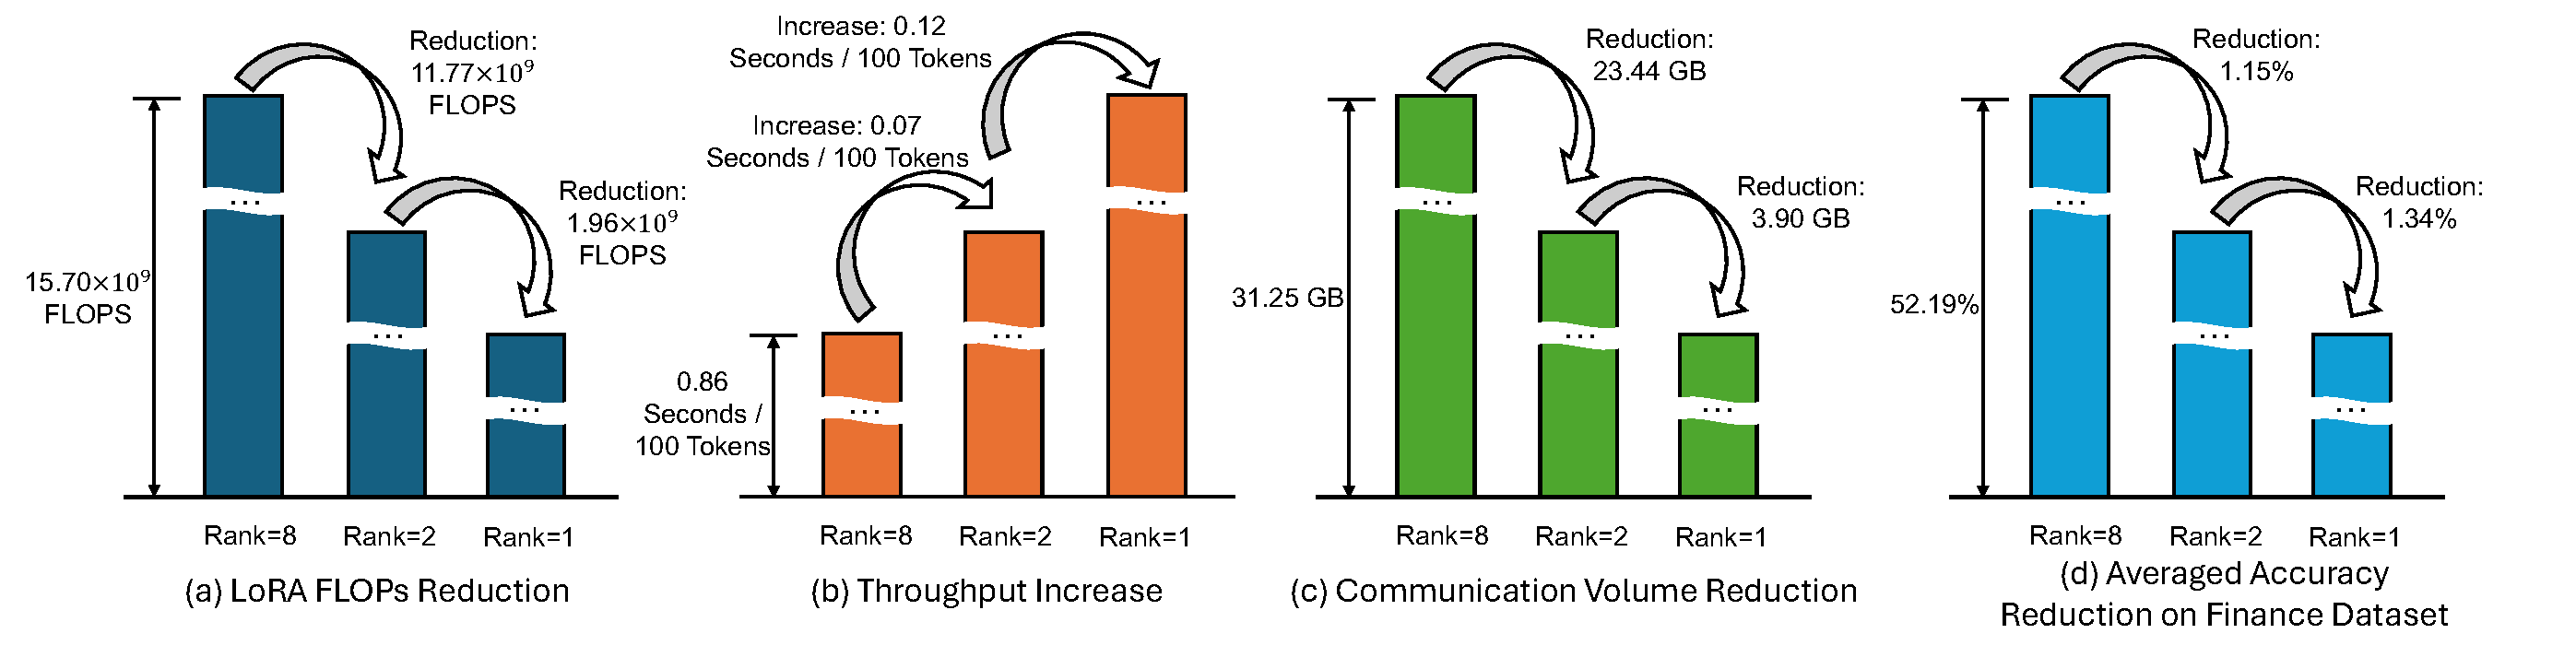
\includegraphics[width=0.98\linewidth]{fig/rank_resources.pdf}
    \caption{Visualization on the efficiency of the rank-based method.}
    \label{fig:vis_eff_rank}
    % \vspace{-10pt}
\end{figure*}

In this section, we demonstrate the efficiency of the rank-based method for resource-constrained devices by analyzing the FLOPs of LoRA modules, overall training throughput, and communication costs under different rank settings. We use the LLaMA-3.1-8B model on the Finance dataset as a representative case (detailed dataset description is shown in Section~\ref{appendixsection:datasets}), with a hidden size of $8192$, a batch size of $4$, and assuming $\text{float32}$ precision, where each parameter occupies $4$ bytes.

To compute the FLOPs introduced by LoRA modules, we begin with the forward computation $z = BAx$, which requires $2r(d_{\text{in}} + d_{\text{out}})$ operations per token, where $r$ is the LoRA rank and $d_{\text{in}} = d_{\text{out}} = d = 8192$ is the hidden dimension. Since the backward pass roughly doubles the compute cost, the total per-token FLOPs for each LoRA module becomes $6rd$. The total LoRA FLOPs per training step can thus be estimated as $6rd \times \text{batch size} \times \text{sequence length} \times \text{number of LoRA modules}$. For instance, with a sequence length of $512$, $32$ transformer layers, $2$ target modules per layer, result in total $64$ LoRA modules, the total becomes $6 \times r \times 8192 \times 4 \times 512 \times 64 = 196{,}608 \times r$ FLOPs. This value increases linearly with rank. 
On the training dataset, in order to train one epoch with the full dataset, it requires approximately $10{,}000$ steps with this batch size (i.e., 4), such that the total FLOPs introduced by LoRA modules under rank settings $r = 8$, $2$, and $1$ are respectively $1.57 \times 10^6 \times 10{,}000 = 1.57 \times 10^{10}$, $3.93 \times 10^5 \times 10{,}000 = 3.93 \times 10^9$, and $1.97 \times 10^5 \times 10{,}000 = 1.97 \times 10^9$ FLOPs per epoch for the LLaMA-3.1-8B model. We visualize the FLOPs reductions for three levels of rank settings in Figure~\ref{fig:vis_eff_rank} (a).

To assess the training efficiency under different LoRA rank settings, we measure the throughput in terms of seconds per 100 tokens. The actual wall-clock times for the whole training process in our setting are 3.07, 2.84, and 2.41 days under rank settings $r = 8$, $2$, and $1$, respectively. The experimental and hardware settings are reported in Sections~\ref{appendixsection:datasets},~\ref{appendixsubsection:main_settings}. This results in throughput values of approximately $0.864$, $0.799$, and $0.678$ seconds per 100 tokens, respectively. These measurements demonstrate that reducing the rank leads to improved computational efficiency during training. 
% It is worth noting that the wall-clock times are measured under our FL simulation environment, on heterogeneous and resource-constrained devices, the actual processing speed can be even slower, potentially amplifying the observed discrepancies.
We visualize the throughput increase for three levels of rank settings in Figure~\ref{fig:vis_eff_rank} (b).

To estimate the communication volume for one training epoch, we assume that only the LoRA parameters are transmitted every 10 steps. With 10,000 steps per epoch and transmission frequency every 10 steps, there are 1,000 transmissions in total. Each transmission involves sending and receiving $128rd$ LoRA module parameters, where $r$ is the LoRA rank and $d = 8192$ is the hidden size. Assuming $\texttt{float32}$ precision (4 bytes per parameter), this yields a total communication volume of $512{,}000rd$ bytes per epoch. For ranks $r = 1$, $2$, and $8$, the resulting communication costs are approximately 3.91 GB, 7.81 GB, and 31.25 GB, respectively. We visualize the communication volume reductions for three levels of rank settings in Figure~\ref{fig:vis_eff_rank} (c).

From the resource consumption perspective, the rank-based method provides a practical solution for efficient federated fine-tuning of LLMs, as evidenced by the reduction in LoRA module FLOPs and communication volume, as well as improved training throughput. Although the rank-based approach is not specifically designed for memory savings, our method is orthogonal to a wide range of existing memory-efficient techniques and can be easily combined with them (as discussed in Section~\ref{appendixsection:relatedworks}).

These resource consumption reductions make low-rank configurations particularly practical for deployment in heterogeneous federated settings. However, as shown in Figure~\ref{fig:vis_eff_rank}~(d), we provide an average performance comparison on Finance datasets under three levels of rank settings. The average accuracies are 52.19\%, 51.04\%, and 50.05\% for ranks $r = 8$, $2$, and $1$, respectively. This demonstrates that different LoRA rank settings lead to a noticeable performance gap, where even a 1\% drop in accuracy is considered significant and typical in LLM instruction fine-tuning tasks on domain-specific downstream datasets. This observation motivates the design of our proposed method, Fed-PLoRA, which aims to incorporate clients experiencing degraded performance under low-rank configurations into a heterogeneous-rank federated training process and improve the overall performance of the global model.


\subsection{Computation, Communication, and Memory Overhead of Fed-PLoRA}\label{appendixsec:overhead_analysis}

We analyze numerical resource overhead in this section. Here, we use HETLoRA~\cite{cho2024heterogeneous} as a reference to calculate overhead, since it is the naive extension of FedAvg to heterogeneous resource settings. We provide the results as following: 


% {\noindent\textbf{Same number of local trainable parameters.}
% For fairness, all methods on the same dataset are configured to use an identical number of local trainable parameters, scaling as $\mathcal{O}((d+k)r_i)$ per client. Under the configurations in Table~\ref{tab:appendix-fl-settings}, the average local parameter budget per client is $0.23$M for BERT-base, $1.39$M for LLaMA~1B, $2.13$M for OPT-1.3B, $1.32$M for Mistral-7B-v0.3, and $1.77$M for Llama-3.1-8B.}

% \begin{table}[h]
% 
% \centering
% \renewcommand{\arraystretch}{1.2}
% \scalebox{0.9}{
% \begin{tabular}{lc}
% \toprule[1.25pt]
% \textbf{Model} & \textbf{Average Local Trainable Parameters (Million)} \\
% \midrule
% BERT-base        & 0.23  \\
% LLaMA-1B         & 1.39  \\
% OPT-1.3B         & 2.13  \\
% Mistral-7B-v0.3  & 1.32  \\
% Llama-3.1-8B     & 1.77  \\
% \bottomrule[1.25pt]
% \end{tabular}
% }
% \caption{{Average local trainable parameter budget per client (same across methods within each dataset).}}
% \label{tab:trainable_params}
% \end{table}

\noindent\textbf{Computation Overhead.}
During the FL process, the computation overhead can be analyzed in the steps of local parameter initialization, local training, and server-side model aggregation~\cite{wu2022node,zhou2022exact}. 
%
% For {local parameter initialization}, our method introduces an additional folding cost. Specifically, in each training round, the unselected LoRA modules, totaling $L \cdot M \cdot (R - r_i)$ parallel one-rank components, are folded into the pretrained model by computing their low-rank projections and adding them to the target weight matrix. Each such component involves multiplying a $d \times r$ matrix with an $r \times d$ matrix, incurring $r \cdot d^2$ FLOPs. The overall folding complexity per round is thus $O(L \cdot M \cdot (R - r_i) \cdot r \cdot d^2)$, where $L$ is the number of transformer layers, $M$ is the number of target modules per layer (e.g., query and value projections), $R$ is the global LoRA rank, $r_i$ is the number of selected one-rank modules on the client, $r$ is the rank of each LoRA component (typically 1 for PLoRA modules), and $d$ is the hidden size. Since $r = 1$ and $R - r_i \ll d$ in our setting, this folding overhead is negligible compared to the full forward and backward pass.
% %
% In contrast, HETLoRA and FlexLoRA impose no local parameter initialization overhead, as clients directly receive pre-initialized LoRA modules from the server without further modification, similar to FedIT.
% %
% FLoRA, on the other hand, stacks all received LoRA updates and applies them jointly to the target weight matrix on the server. The associated computation depends on the total rank accumulated from all selected clients. 
% In the worst case, if all $10$ participating clients upload LoRA modules with rank $R=16$, the server-side update cost becomes $O(L \cdot M \cdot 10 \cdot R \cdot d^2)$. This introduces a scalability bottleneck in FLoRA, as its aggregation cost grows linearly with the number of participating clients.
%
% Numerically, for example, in BERT-base ($L=12$, $d=768$, $M=2$), the folding overhead in our method is approximately $12 \cdot 2 \cdot (16 - 1) \cdot 768^2 = 2.1 \times 10^8$ FLOPs per round. Under the same configuration, FLoRA's server-side aggregation cost reaches $12 \cdot 2 \cdot 10 \cdot 16 \cdot 768^2 = 2.2 \times 10^{9}$ FLOPs per round.
%
% For {local training} overhead, all methods involve the same FLOPs as FedIT, resulting in no additional computational overhead during training.
%
% During {model aggregation}, our method, HETLoRA, and FLoRA only involve element-wise addition operations between local updates, resulting in negligible aggregation overhead compared to FedIT. Note that FLoRA performs local matrix operations over LoRA modules to reduce communication cost, so its aggregation process slightly differs from the one illustrated in Figure~\ref{fig:framework}. In contrast, FlexLoRA aggregates the received LoRA modules by first converting all low-rank updates into full matrices, summing them, and then applying a SVD to project the result back to the target rank. Formally, if $W_i = B_i A_i$ is the LoRA update from client $i$, FlexLoRA computes $\sum_{i=1}^{K} W_i$ and performs SVD on the result to obtain a compressed update of rank $R$. In the worst-case scenario where $K$ clients each upload LoRA modules of rank $R$, and the aggregated matrix is also decomposed back to rank $R$, the aggregation involves constructing a full $d \times d$ matrix, summing $K$ such matrices, and computing SVD, which incurs $O(d^3)$ complexity. 
% For BERT-base ($d=768$), this results in approximately $768^3 = 4.5 \times 10^8$ FLOPs per aggregation step.
%
{To ground the discussion, we report the per-client, per-round computational workloads under BERT-base~\cite{devlin2019bert} with PF16 precision. The results (in terms of FLOPs) are reported using 100 clients with a global rank of $R{=}16$ and a local rank configuration of $\{1,4,16\}$, representing three tiers of resource heterogeneity. The number of clients in each tier are 34, 33, and 33, respectively. Each client is assigned 100 training samples. The result are summarized in Table~\ref{tab:compute_overhead}. Note that, because local initialization, local training, and local overhead vary across clients, we report the results for the weakest client with $r_i=1$, as it represents the most resource-constrained setting.
}

\begin{table}[h]

\centering
\renewcommand{\arraystretch}{1.3}
\scalebox{0.52}{
\begin{tabular}{
    >{\centering\arraybackslash}m{3.5cm}
    >{\centering\arraybackslash}m{4.5cm}
    >{\centering\arraybackslash}m{4.5cm}
    >{\centering\arraybackslash}m{5cm}
    >{\centering\arraybackslash}m{3.5cm}
    >{\centering\arraybackslash}m{3.5cm}
}
\toprule[1.3pt]
\textbf{Method} & \textbf{Local Initialization (FLOPs) } & \textbf{Local Training (FLOPs)}  & \textbf{Model Aggregation (FLOPs)} 
& \textbf{Local Overhead (FLOPs)} & \textbf{Server Overhead (FLOPs)}
\\
\midrule
HETLoRA
& $3.68\times10^4$
&  $1.45\times10^{14}$
& $2.94\times10^7$
& -
& -
\\
\midrule
FLoRA
& $6.26\times10^5$
& $1.45\times10^{14}$
& $8.88\times10^9$
& $+5.89\times10^5$
& $+8.85\times10^9$
\\
FlexLoRA
& $3.68\times10^4$
& $1.45\times10^{14}$
& $7.71\times10^{10}$
& None
& $+7.70\times10^{10}$
\\\midrule
\textbf{Fed–PLoRA (Ours)}
& $1.41\times10^7$
& $1.45\times10^{14}$
& $1.10\times10^6$
& $+1.40\times10^7$
& $-2.83\times10^7$
\\
\bottomrule[1.3pt]
\end{tabular}
}
\caption{{Computation overhead of Fed-PLoRA compared with SOTA methods.}}
\label{tab:compute_overhead}
\end{table}

{Overall, the dominant computation cost arises from local training, which on the order of $10^{14}$ FLOPs. Our method adds only negligible overhead during local initialization (on the order of $10^{7}$ FLOPs), and reduces computational cost for model aggregation compared to HETLoRA.
}




{\noindent\textbf{Communication Overhead.}
The communication cost accounts for both uplink and downlink traffic.}
% , with uplink being particularly important due to its effect on client–server connectivity~\cite{mhanna2024countering}. 
% For all methods, the uplink remains identical to HETLoRA since each client uploads only its trainable LoRA modules.}
% For downlink traffic of Fed-PLoRA, instead of sending only the global LoRA module with rank $r_i$, the server broadcasts all $R$ one-rank PLoRA modules so that clients can fold them selectively. 
%
{Here, we report the per-client, per-round uplink and downlink volumes. The measurements are obtained using FP16 BERT-base~\cite{devlin2019bert} with a global rank of $R{=}16$. In Table ~\ref{tab:comm_overhead}, we report the results for the weakest client with $r_i=1$, which reflects the largest communication overhead incurred by our method.}

\begin{table}[h]

\centering
\renewcommand{\arraystretch}{1.35}
\scalebox{0.75}{
\begin{tabular}{cccc}
\toprule[1pt]
\textbf{Method} & \textbf{Uplink (MB)} & \textbf{Downlink (MB)} & \textbf{Overhead (MB)} \\
\midrule
HETLoRA &
0.04 &
0.04 &
-
\\
\midrule
FLoRA &
0.04
& 13.54
&+13.50
\\
FlexLoRA 
& 0.04
& 0.04
& None 
\\
\midrule
\textbf{Fed–PLoRA (Ours)} 
&0.04 &
0.54 &
+0.50
\\
\bottomrule[1pt]
\end{tabular}
}
\vspace{-4pt}
\caption{{Communication overhead of Fed-PLoRA compared with SOTA methods.}}
\label{tab:comm_overhead}
\end{table}

{We can see that our method incurs only 0.50 MB of overhead per round for the weakest client, which is negligible even in constrained network settings.
We further extend our evaluation to larger models when analyzing the downlink traffic of Fed-PLoRA. As shown in Table~\ref{tab:downlink_traffic}, in Fed-PLoRA, the downlink traffic is only a few megabytes per round per client, even for models with billions of parameters, making it easily deployable over low-bandwidth networks.}

\begin{table}[h]

\centering
\renewcommand{\arraystretch}{1.15}
\scalebox{0.78}{
\begin{tabular}{lc}
\toprule[1.15pt]
\textbf{Model} & \textbf{Downlink (MB)} \\ \midrule
% BERT-base                     & 0.54 \\
LLaMA-1B                      & 2.79 \\
OPT-1.3B                      & 2.62 \\
Mistral-7B-v0.3               & 7.08 \\
Llama-3.1-8B                  & 7.09 \\
Qwen3-4B-Instruct-2507        & 5.24 \\
\bottomrule[1.15pt]
\end{tabular}
}
\caption{{Downlink traffic of Fed–PLoRA across model scales.}}
\label{tab:downlink_traffic}
\end{table}

% {Overall, Fed–PLoRA provides a strong communication–performance tradeoff, improving training stability while maintaining practical bandwidth usage.}


\begin{table}[h]

\centering
\renewcommand{\arraystretch}{1.25}
\scalebox{0.50}{
\begin{tabular}{lccccc}
\toprule[1.25pt]
\textbf{Method} 
& \textbf{Persistent Base Model (MB)} 
& \textbf{Persistent Local Trainable Parameters (MB)} 
& \textbf{Temporary Global Parameters (MB)} 
& \textbf{Local Training (MB)} 
& \textbf{Total Overhead (MB)}
\\
\midrule
HETLoRA
& 210.00
& 0.04
& 0.04 $\rightarrow$ 0
& 2717.91
& - \\
\midrule
FLoRA
& 210.00
& 0.04
& 13.54 $\rightarrow$ 0
& 2717.91
& +13.50 $\rightarrow$ 0 \\
FlexLoRA
& 210.00
& 0.04
& 0.04 $\rightarrow$ 0
& 2717.91
& None \\
\textbf{Fed–PLoRA (Ours)}
& 210.00
& 0.04
& 0.54 $\rightarrow$ 0
& 2717.91
& +0.50 $\rightarrow$ 0  \\
\bottomrule[1.25pt]
\end{tabular}
}
\caption{{Memory overhead of Fed-PLoRA compared with SOTA methods.}}
\label{tab:memory_overhead}
\end{table}

\noindent\textbf{Memory Overhead.} { Here, we study the memory usage for the storage of the base model and local trainable LoRA/PLoRA parameters, the temporary memory for the received global parameters during local initialization, and the memory during local training. The results are obtained using FP16 BERT-base~\cite{devlin2019bert} with a global rank of $R{=}16$. The batch size for local training is 16, and the input size is 512. We report the memory footprint on the weakest client with rank $r_i=1$ in Table~\ref{tab:memory_overhead}. The persistent base model and local LoRA/PLoRA parameters occupy the same amount of memory across all methods. When dealing with the received global parameters during local initialization, our method requires addtional 0.50 MB of temporary memory, which is negligible compared to the base model’s and local training memory costs.}

% The memory usage on each client $i$ including the storage of the base model, memory cost of each client’s LoRA/PLoRA modules, the temporary memory buffer used during local initialization, and memory required during local training.
%
% The client-side storage overhead includes both the received global model and temporary storage for intermediate parameters. In our method, each client receives all $R$ PLoRA modules from the server but only trains a subset of $r_i$ modules. The remaining $(R - r_i)$ modules are folded into the pre-trained target modules and remain frozen. Since the modified target module $\boldsymbol{\mathcal{W}}_i^t$ can be reconstructed from $\boldsymbol{\mathcal{W}}^0$ after training, it does not incur additional storage overhead. Therefore, the temporary net extra storage compared to FedIT is $(R - r_i)$ LoRA modules per client. 
% % For the BERT-base configuration ($L = 12$, $d = 768$, $M = 2$), this corresponds to approximately $276{,}480$ parameters, or around $1.05$\,MB in 32-bit precision when $R = 16$ and $r_i = 1$.
% %
% In contrast, {FLoRA} requires each client to store all LoRA modules selected by clients in the previous round, which may not overlap with their own selection. This leads to significantly higher client-side storage demands in heterogeneous settings. In the worst case where all clients use only a single module ($r_i = 1$), FLoRA incurs a storage overhead of $(K \cdot R - 1)$ LoRA modules.
% % , or about $11.18$\,MB per client under the same configuration.
% %
% {HETLoRA} and {FlexLoRA} follow a different design: each client receives and stores only the LoRA parameters it needs to train, without additional modules. As a result, their client-side storage footprint is minimal and equivalent to FedIT. However, this minimal overhead comes at the cost of potential initialization noise, especially when client rank configurations differ significantly.
%

% {Overall}, our method introduces a modest overhead in client-side storage to reduce initialization noise.




% {Overall, Fed-PLoRA imposes negligible overhead in communication, computation, and memory, which is deployment-friendly under FL framework.
% }

\end{document}

